% Options for packages loaded elsewhere
\PassOptionsToPackage{unicode}{hyperref}
\PassOptionsToPackage{hyphens}{url}
\PassOptionsToPackage{dvipsnames,svgnames,x11names}{xcolor}
%
\documentclass[
  10pt,
  a4paper,
]{article}

\usepackage{amsmath,amssymb}
\usepackage{iftex}
\ifPDFTeX
  \usepackage[T1]{fontenc}
  \usepackage[utf8]{inputenc}
  \usepackage{textcomp} % provide euro and other symbols
\else % if luatex or xetex
  \usepackage{unicode-math}
  \defaultfontfeatures{Scale=MatchLowercase}
  \defaultfontfeatures[\rmfamily]{Ligatures=TeX,Scale=1}
\fi
\usepackage{lmodern}
\ifPDFTeX\else  
    % xetex/luatex font selection
\fi
% Use upquote if available, for straight quotes in verbatim environments
\IfFileExists{upquote.sty}{\usepackage{upquote}}{}
\IfFileExists{microtype.sty}{% use microtype if available
  \usepackage[]{microtype}
  \UseMicrotypeSet[protrusion]{basicmath} % disable protrusion for tt fonts
}{}
\makeatletter
\@ifundefined{KOMAClassName}{% if non-KOMA class
  \IfFileExists{parskip.sty}{%
    \usepackage{parskip}
  }{% else
    \setlength{\parindent}{0pt}
    \setlength{\parskip}{6pt plus 2pt minus 1pt}}
}{% if KOMA class
  \KOMAoptions{parskip=half}}
\makeatother
\usepackage{xcolor}
\usepackage[top=18mm,bottom=15mm,left=5mm,right=5mm]{geometry}
\usepackage{soul}
\setlength{\emergencystretch}{3em} % prevent overfull lines
\setcounter{secnumdepth}{-\maxdimen} % remove section numbering
% Make \paragraph and \subparagraph free-standing
\ifx\paragraph\undefined\else
  \let\oldparagraph\paragraph
  \renewcommand{\paragraph}[1]{\oldparagraph{#1}\mbox{}}
\fi
\ifx\subparagraph\undefined\else
  \let\oldsubparagraph\subparagraph
  \renewcommand{\subparagraph}[1]{\oldsubparagraph{#1}\mbox{}}
\fi

\usepackage{color}
\usepackage{fancyvrb}
\newcommand{\VerbBar}{|}
\newcommand{\VERB}{\Verb[commandchars=\\\{\}]}
\DefineVerbatimEnvironment{Highlighting}{Verbatim}{commandchars=\\\{\}}
% Add ',fontsize=\small' for more characters per line
\newenvironment{Shaded}{}{}
\newcommand{\AlertTok}[1]{\textcolor[rgb]{1.00,0.33,0.33}{\textbf{#1}}}
\newcommand{\AnnotationTok}[1]{\textcolor[rgb]{0.42,0.45,0.49}{#1}}
\newcommand{\AttributeTok}[1]{\textcolor[rgb]{0.84,0.23,0.29}{#1}}
\newcommand{\BaseNTok}[1]{\textcolor[rgb]{0.00,0.36,0.77}{#1}}
\newcommand{\BuiltInTok}[1]{\textcolor[rgb]{0.84,0.23,0.29}{#1}}
\newcommand{\CharTok}[1]{\textcolor[rgb]{0.01,0.18,0.38}{#1}}
\newcommand{\CommentTok}[1]{\textcolor[rgb]{0.42,0.45,0.49}{#1}}
\newcommand{\CommentVarTok}[1]{\textcolor[rgb]{0.42,0.45,0.49}{#1}}
\newcommand{\ConstantTok}[1]{\textcolor[rgb]{0.00,0.36,0.77}{#1}}
\newcommand{\ControlFlowTok}[1]{\textcolor[rgb]{0.84,0.23,0.29}{#1}}
\newcommand{\DataTypeTok}[1]{\textcolor[rgb]{0.84,0.23,0.29}{#1}}
\newcommand{\DecValTok}[1]{\textcolor[rgb]{0.00,0.36,0.77}{#1}}
\newcommand{\DocumentationTok}[1]{\textcolor[rgb]{0.42,0.45,0.49}{#1}}
\newcommand{\ErrorTok}[1]{\textcolor[rgb]{1.00,0.33,0.33}{\underline{#1}}}
\newcommand{\ExtensionTok}[1]{\textcolor[rgb]{0.84,0.23,0.29}{\textbf{#1}}}
\newcommand{\FloatTok}[1]{\textcolor[rgb]{0.00,0.36,0.77}{#1}}
\newcommand{\FunctionTok}[1]{\textcolor[rgb]{0.44,0.26,0.76}{#1}}
\newcommand{\ImportTok}[1]{\textcolor[rgb]{0.01,0.18,0.38}{#1}}
\newcommand{\InformationTok}[1]{\textcolor[rgb]{0.42,0.45,0.49}{#1}}
\newcommand{\KeywordTok}[1]{\textcolor[rgb]{0.84,0.23,0.29}{#1}}
\newcommand{\NormalTok}[1]{\textcolor[rgb]{0.14,0.16,0.18}{#1}}
\newcommand{\OperatorTok}[1]{\textcolor[rgb]{0.14,0.16,0.18}{#1}}
\newcommand{\OtherTok}[1]{\textcolor[rgb]{0.44,0.26,0.76}{#1}}
\newcommand{\PreprocessorTok}[1]{\textcolor[rgb]{0.84,0.23,0.29}{#1}}
\newcommand{\RegionMarkerTok}[1]{\textcolor[rgb]{0.42,0.45,0.49}{#1}}
\newcommand{\SpecialCharTok}[1]{\textcolor[rgb]{0.00,0.36,0.77}{#1}}
\newcommand{\SpecialStringTok}[1]{\textcolor[rgb]{0.01,0.18,0.38}{#1}}
\newcommand{\StringTok}[1]{\textcolor[rgb]{0.01,0.18,0.38}{#1}}
\newcommand{\VariableTok}[1]{\textcolor[rgb]{0.89,0.38,0.04}{#1}}
\newcommand{\VerbatimStringTok}[1]{\textcolor[rgb]{0.01,0.18,0.38}{#1}}
\newcommand{\WarningTok}[1]{\textcolor[rgb]{1.00,0.33,0.33}{#1}}

\providecommand{\tightlist}{%
  \setlength{\itemsep}{0pt}\setlength{\parskip}{0pt}}\usepackage{longtable,booktabs,array}
\usepackage{calc} % for calculating minipage widths
% Correct order of tables after \paragraph or \subparagraph
\usepackage{etoolbox}
\makeatletter
\patchcmd\longtable{\par}{\if@noskipsec\mbox{}\fi\par}{}{}
\makeatother
% Allow footnotes in longtable head/foot
\IfFileExists{footnotehyper.sty}{\usepackage{footnotehyper}}{\usepackage{footnote}}
\makesavenoteenv{longtable}
\usepackage{graphicx}
\makeatletter
\def\maxwidth{\ifdim\Gin@nat@width>\linewidth\linewidth\else\Gin@nat@width\fi}
\def\maxheight{\ifdim\Gin@nat@height>\textheight\textheight\else\Gin@nat@height\fi}
\makeatother
% Scale images if necessary, so that they will not overflow the page
% margins by default, and it is still possible to overwrite the defaults
% using explicit options in \includegraphics[width, height, ...]{}
\setkeys{Gin}{width=\maxwidth,height=\maxheight,keepaspectratio}
% Set default figure placement to htbp
\makeatletter
\def\fps@figure{htbp}
\makeatother

\usepackage{amssymb, amsmath}

\makeatletter
\renewcommand*\env@matrix[1][\arraystretch]{%
  \edef\arraystretch{#1}%
  \hskip -\arraycolsep
  \let\@ifnextchar\new@ifnextchar
  \array{*\c@MaxMatrixCols c}}
\makeatother


\numberwithin{equation}{section}

\usepackage[utf8]{inputenc}
\usepackage{lastpage} % counts all the pages, used in footer
\usepackage{hyperref}

\usepackage{tikz}
\usetikzlibrary{arrows.meta}

% TIKS TEMPLATES
\tikzset{
dot/.style = {circle, fill, minimum size=#1,
              inner sep=0pt, outer sep=0pt},
dot/.default = 4pt % size of the circle diameter 
}
\tikzset{
sum/.style = {circle, draw=black, inner sep=-0.5pt}
}

\tikzset{
box/.style = {rectangle, draw=black, minimum width = #1},
box/.default = 1cm, % size of the circle diameter 
}




\usepackage{gensymb}

\usepackage{xfrac}

% Flexible Multicolumn Option
\usepackage{multicol}
\setlength\columnsep{20pt}

% Package for enabling colors (colorful output)
\usepackage[dvipsnames]{xcolor}
\definecolor{darkgreen}{HTML}{014f32}

% Icons - http://mirrors.ctan.org/fonts/fontawesome5/doc/fontawesome5.pdf
\usepackage{fontawesome5}

% removes spacing in display math
\usepackage[nodisplayskipstretch]{setspace}

\usepackage{tabularx}

% Font Configuration
\usepackage{lmodern}
\renewcommand{\familydefault}{\sfdefault}
\usepackage{cmbright}
\usepackage[scaled=0.9]{inconsolata}

% 
\usepackage{fancyhdr}

\renewcommand{\headrulewidth}{1pt}
\renewcommand{\footrulewidth}{1pt}

\pagestyle{fancy}
\fancyhead{} % clear all header fields
\makeatletter
\fancyhead[R]{\@title}
\makeatother
\fancyhead[L]{HSLU T\&A}
\fancyfoot{} % clear all footer fields
\fancyfoot[C]{\thepage\ / \pageref{LastPage}}
\fancyfoot[R]{RGT}
\fancyfoot[L]{\today}

% introduces conditions environment to create nice equation parameter descriptions
\usepackage{array}

\newenvironment{conditions}
  {\par\vspace{\abovedisplayskip}\noindent\begin{tabular}{>{$}l<{$} @{${}:{}$} l}}
  {\end{tabular}\par\vspace{\belowdisplayskip}}
  

% Used for pandoc code block generations.
% Introduces breaklines for overflowing code blocks, by defining the Highlighting environment with breakline & symbol.
% Don't know what commandchars does :)
\usepackage{fvextra}
\DefineVerbatimEnvironment{Highlighting}{Verbatim}{
  breaklines=true,
  breakanywhere=true,
  breaksymbolleft={\textcolor{gray}{\scriptsize\ensuremath\hookrightarrow}},
  commandchars=\\\{\}
}



\let\paragraph\oldparagraph
\let\subparagraph\oldsubparagraph

\usepackage{xhfill}
\usepackage[explicit]{titlesec}
\renewcommand{\paragraph}[1]{\oldparagraph{#1}\mbox{}\par}

\titleformat{\section}[block]{\bfseries\Large}{\thetitle.}{3mm}{#1\space\xrfill[0.6ex]{1pt}}


\usepackage{pdfpages}
\usepackage{float}
\makeatletter
\let\oldlt\longtable
\let\endoldlt\endlongtable
\def\longtable{\@ifnextchar[\longtable@i \longtable@ii}
\def\longtable@i[#1]{\begin{figure}[H]
\onecolumn
\begin{minipage}{0.5\textwidth}
\oldlt[#1]
}
\def\longtable@ii{\begin{figure}[H]
\onecolumn
\begin{minipage}{0.5\textwidth}
\oldlt
}
\def\endlongtable{\endoldlt
\end{minipage}
\twocolumn
\end{figure}}
\makeatother
\usepackage[nswissgerman]{babel}
\makeatletter
\@ifpackageloaded{tcolorbox}{}{\usepackage[skins,breakable]{tcolorbox}}
\@ifpackageloaded{fontawesome5}{}{\usepackage{fontawesome5}}
\definecolor{quarto-callout-color}{HTML}{909090}
\definecolor{quarto-callout-note-color}{HTML}{0758E5}
\definecolor{quarto-callout-important-color}{HTML}{CC1914}
\definecolor{quarto-callout-warning-color}{HTML}{EB9113}
\definecolor{quarto-callout-tip-color}{HTML}{00A047}
\definecolor{quarto-callout-caution-color}{HTML}{FC5300}
\definecolor{quarto-callout-color-frame}{HTML}{acacac}
\definecolor{quarto-callout-note-color-frame}{HTML}{4582ec}
\definecolor{quarto-callout-important-color-frame}{HTML}{d9534f}
\definecolor{quarto-callout-warning-color-frame}{HTML}{f0ad4e}
\definecolor{quarto-callout-tip-color-frame}{HTML}{02b875}
\definecolor{quarto-callout-caution-color-frame}{HTML}{fd7e14}
\makeatother
\makeatletter
\makeatother
\makeatletter
\makeatother
\makeatletter
\@ifpackageloaded{caption}{}{\usepackage{caption}}
\AtBeginDocument{%
\ifdefined\contentsname
  \renewcommand*\contentsname{Inhaltsverzeichnis}
\else
  \newcommand\contentsname{Inhaltsverzeichnis}
\fi
\ifdefined\listfigurename
  \renewcommand*\listfigurename{Abbildungsverzeichnis}
\else
  \newcommand\listfigurename{Abbildungsverzeichnis}
\fi
\ifdefined\listtablename
  \renewcommand*\listtablename{Tabellenverzeichnis}
\else
  \newcommand\listtablename{Tabellenverzeichnis}
\fi
\ifdefined\figurename
  \renewcommand*\figurename{Abbildung}
\else
  \newcommand\figurename{Abbildung}
\fi
\ifdefined\tablename
  \renewcommand*\tablename{Tabelle}
\else
  \newcommand\tablename{Tabelle}
\fi
}
\@ifpackageloaded{float}{}{\usepackage{float}}
\floatstyle{ruled}
\@ifundefined{c@chapter}{\newfloat{codelisting}{h}{lop}}{\newfloat{codelisting}{h}{lop}[chapter]}
\floatname{codelisting}{Listing}
\newcommand*\listoflistings{\listof{codelisting}{Listingverzeichnis}}
\makeatother
\makeatletter
\@ifpackageloaded{caption}{}{\usepackage{caption}}
\@ifpackageloaded{subcaption}{}{\usepackage{subcaption}}
\makeatother
\makeatletter
\@ifpackageloaded{tcolorbox}{}{\usepackage[skins,breakable]{tcolorbox}}
\makeatother
\makeatletter
\@ifundefined{shadecolor}{\definecolor{shadecolor}{rgb}{.97, .97, .97}}
\makeatother
\makeatletter
\@ifundefined{codebgcolor}{\definecolor{codebgcolor}{HTML}{f7f7f7}}
\makeatother
\makeatletter
\makeatother
\ifLuaTeX
  \usepackage{selnolig}  % disable illegal ligatures
\fi
\IfFileExists{bookmark.sty}{\usepackage{bookmark}}{\usepackage{hyperref}}
\IfFileExists{xurl.sty}{\usepackage{xurl}}{} % add URL line breaks if available
\urlstyle{same} % disable monospaced font for URLs
\hypersetup{
  pdftitle={Regelungstechnik},
  pdfauthor={Joel von Rotz},
  colorlinks=true,
  linkcolor={blue},
  filecolor={Maroon},
  citecolor={Blue},
  urlcolor={Blue},
  pdfcreator={LaTeX via pandoc}}

\title{Regelungstechnik}
\author{Joel von Rotz}
\date{Invalid Date}

\begin{document}
 % [START] title
 % [ELSE] beamer

\makeatletter
\begin{center}
  \vspace*{0.5cm}
  
  \textbf{\Huge \@title}\\
  \vspace{0.1cm}
  \textsf{\textit{\large Zusammenfassung}}
  
  \vspace{0.5cm}

  \textsf{\large \@author \hspace{0.3cm}\textbf{/}\hspace{0.3cm}\large \faGithub\space \href{https://github.com/joelvonrotz/bachelor-electrical-engineering/tree/main/semester\%204/summary/regelungstechnik}{Quelldateien}}
  

\end{center}
\makeatother

 % [END] beamer
 % [END] title
\ifdefined\Shaded\renewenvironment{Shaded}{\begin{tcolorbox}[frame hidden, breakable, enhanced, colback={codebgcolor}, boxrule=0pt, borderline west={3pt}{0pt}{shadecolor}, sharp corners]}{\end{tcolorbox}}\fi

\renewcommand*\contentsname{Inhaltsverzeichnis}
{
\hypersetup{linkcolor=}
\setcounter{tocdepth}{3}
\tableofcontents
}
\newpage

\begin{tcolorbox}[enhanced jigsaw, opacitybacktitle=0.6, coltitle=black, arc=.35mm, title=\textcolor{quarto-callout-tip-color}{\faLightbulb}\hspace{0.5em}{Vorgehen MEP}, opacityback=0, colframe=quarto-callout-tip-color-frame, left=2mm, bottomtitle=1mm, toptitle=1mm, toprule=.15mm, breakable, leftrule=.75mm, colback=white, titlerule=0mm, bottomrule=.15mm, rightrule=.15mm, colbacktitle=quarto-callout-tip-color!10!white]

\begin{itemize}
\tightlist
\item
  Zuerst lösen, was man kann und nicht zu lange Zeit verlieren
\item
  10 Minuten pro Aufgabe

  \begin{itemize}
  \tightlist
  \item
    Gewisse Aufgaben brauchen mehr als 10 Minuten, andere weniger
  \end{itemize}
\item
  Aufgaben sind meist einfacher als man denkt

  \begin{itemize}
  \tightlist
  \item
    Es gibt verschiedene Lösungsansätze
  \item
    Annahmen treffen oder fragen, falls man unsicher ist
  \end{itemize}
\item
  Wenn Zeit übrig, Lösung validieren
\end{itemize}

\end{tcolorbox}

% keep this to have smaller code blocks
\ifdefined\Shaded\renewenvironment{Shaded}{\begin{tcolorbox}[
  colback={shadecolor},
  boxrule=0pt,
  left=3pt,
  right=3pt,
  top=3pt,
  bottom=3pt,
  frame hidden,
  enhanced,
  breakable
]}{\end{tcolorbox}}\fi

\begin{multicols*}{2}

\hypertarget{kurzfassung}{%
\section{Kurzfassung}\label{kurzfassung}}

\hypertarget{linear-algebra}{%
\subsection{Linear Algebra}\label{linear-algebra}}

\hypertarget{determinante}{%
\subsubsection{Determinante}\label{determinante}}

\hypertarget{times-2-matrix}{%
\paragraph{\texorpdfstring{2 \(\times\)
2-Matrix}{2 \textbackslash times 2-Matrix}}\label{times-2-matrix}}

\[
\det(A)=\begin{vmatrix} \textcolor{BurntOrange}{a} & b \\c & \textcolor{BurntOrange}{d}\end{vmatrix} ={\textcolor{BurntOrange}{ad}-bc}
\]

\hypertarget{times-3-matrix}{%
\paragraph{\texorpdfstring{3 \(\times\)
3-Matrix}{3 \textbackslash times 3-Matrix}}\label{times-3-matrix}}

\[
\det(A)=\begin{vmatrix} \textcolor{BurntOrange}{a} & \textcolor{NavyBlue}{b} & \textcolor{OliveGreen}{c} \\ \textcolor{OliveGreen}{d} & \textcolor{BurntOrange}{e} & \textcolor{NavyBlue}{f} \\ \textcolor{NavyBlue}{g} & \textcolor{OliveGreen}{h} & \textcolor{BurntOrange}{i} \end{vmatrix} = \textcolor{BurntOrange}{aei}+\textcolor{NavyBlue}{bfg}+\textcolor{OliveGreen}{cdh}-ceg-bdi-afh
\]

\hypertarget{inverse-matrix}{%
\subsubsection{Inverse Matrix}\label{inverse-matrix}}

\[
A^{-1}=\frac{\text{adj}(A)}{\det(A)}
\]

\hypertarget{times-2-matrix-1}{%
\paragraph{\texorpdfstring{2 \(\times\)
2-Matrix}{2 \textbackslash times 2-Matrix}}\label{times-2-matrix-1}}

\[
A^{-1}=
\begin{bmatrix} 
\textcolor{BurntOrange}{a} & b \\
c & \textcolor{BrickRed}{d}
\end{bmatrix}^{-1} =
\frac1{\textcolor{BurntOrange}{a}\textcolor{BrickRed}{d}-bc}\cdot
\begin{bmatrix}
\textcolor{BrickRed}{d} & -b \\
-c & \textcolor{BurntOrange}{a}
\end{bmatrix}
\]

\hypertarget{times-3-matrix-1}{%
\paragraph{\texorpdfstring{3 \(\times\)
3-Matrix}{3 \textbackslash times 3-Matrix}}\label{times-3-matrix-1}}

\[
A^{-1}=
\begin{bmatrix} 
a & b & c \\ d & e & f \\ g & h & i
\end{bmatrix}^{-1} = \frac1{\det A} \cdot
\begin{bmatrix}
\small{ei-fh} & \small{ch-bi} & \small{bf-ce} \\
\small{fg-di} & \small{ai-cg} & \small{cd-af} \\
\small{dh-eg} & \small{bg-ah} & \small{ae-bd}
\end{bmatrix}
\]

\hypertarget{signal-system}{%
\subsection{Signal \& System}\label{signal-system}}

\begin{tcolorbox}[enhanced jigsaw, opacitybacktitle=0.6, coltitle=black, arc=.35mm, title=\textcolor{quarto-callout-important-color}{\faExclamation}\hspace{0.5em}{Gültigkeit End- \& Anfangswertsatz}, opacityback=0, colframe=quarto-callout-important-color-frame, left=2mm, bottomtitle=1mm, toptitle=1mm, toprule=.15mm, breakable, leftrule=.75mm, colback=white, titlerule=0mm, bottomrule=.15mm, rightrule=.15mm, colbacktitle=quarto-callout-important-color!10!white]

End- \& Anfangswertsatz gilt nur bei stabilen Systemen.

\end{tcolorbox}

\hypertarget{endwertsatz}{%
\subsubsection{Endwertsatz}\label{endwertsatz}}

\hypertarget{laplace}{%
\paragraph{Laplace}\label{laplace}}

\[
\lim_{t\rightarrow\infty}x(t)=\lim_{s\rightarrow0} s\cdot X(s)
\]

falls \(\lim_{t\rightarrow\infty} x(t)\) existiert

\hypertarget{z-transformation}{%
\paragraph{Z-Transformation}\label{z-transformation}}

\[
\lim_{k\rightarrow\infty}x[k]=\lim_{z\rightarrow1}(z-1)X(z)
\]

falls \(X(z)\) nur Pole mit \(\lvert z\rvert < 1\) oder bei \(z=1\)

\hypertarget{anfangswertsatz}{%
\subsubsection{Anfangswertsatz}\label{anfangswertsatz}}

\hypertarget{laplace-1}{%
\paragraph{Laplace}\label{laplace-1}}

\[
x(0^+)=\lim_{s\rightarrow\infty}s\cdot X(s)
\]

falls \(x(0^+)\) existiert

\hypertarget{z-transformation-1}{%
\subsubsection{Z-Transformation}\label{z-transformation-1}}

\[
x[0]=\lim_{z\rightarrow\infty}X(z)
\]

\hypertarget{transformationen}{%
\subsection{Transformationen}\label{transformationen}}

\hypertarget{laplace-2}{%
\subsubsection{Laplace}\label{laplace-2}}

\begin{figure}[H]

{\centering 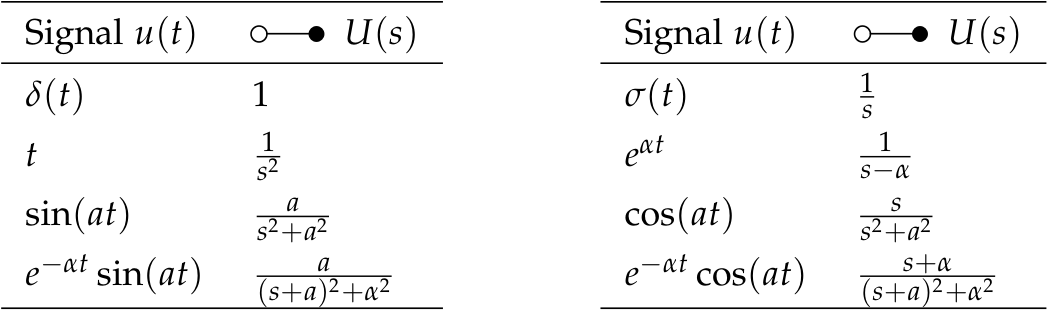
\includegraphics{images/paste-17.png}

}

\end{figure}

\hypertarget{z-transformation-2}{%
\subsubsection{Z-Transformation}\label{z-transformation-2}}

\begin{figure}[H]

{\centering 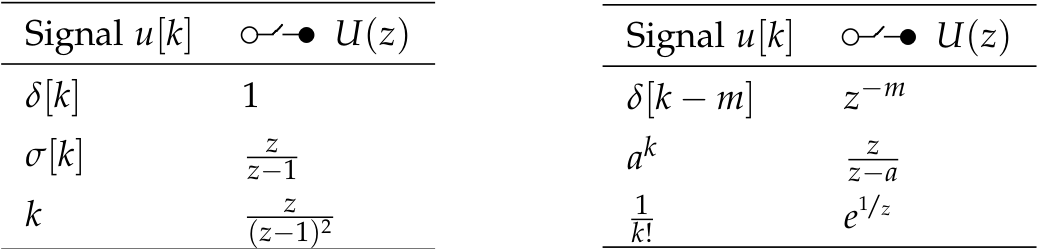
\includegraphics{images/paste-18.png}

}

\end{figure}

\hypertarget{euler-approximation}{%
\subsection{Euler Approximation}\label{euler-approximation}}

\begin{figure}[H]

{\centering 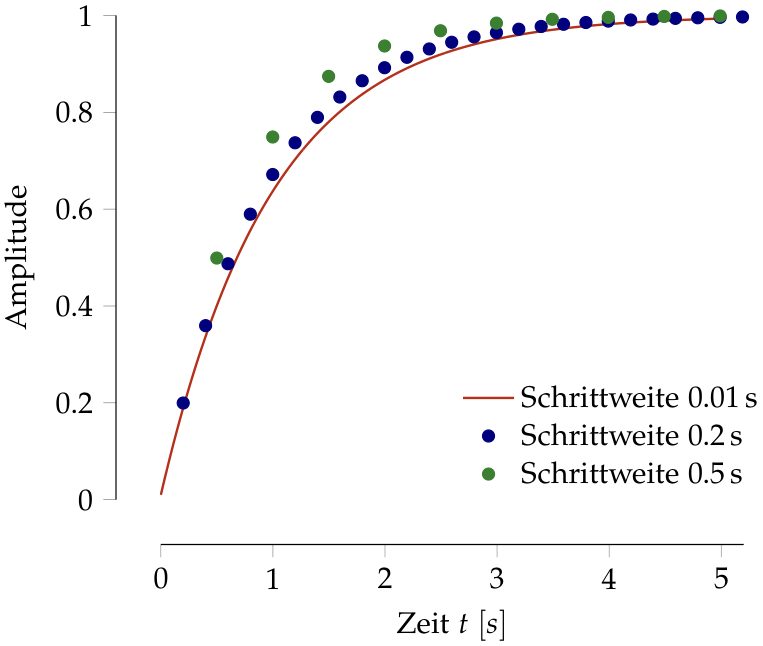
\includegraphics[width=6cm,height=\textheight]{images/paste-32.png}

}

\end{figure}

\[
\begin{split}
x(t+h) &\approx x(t) + h\frac{dx}{dt}=x(t)+h\cdot f(x(t),u(t)) \\
x[k+1] &\approx x[k] + h\cdot f(x[k],u[k])
\end{split}
\]

\hypertarget{systeme}{%
\section{Systeme}\label{systeme}}

\hypertarget{grundlegende-systeme}{%
\subsection{Grundlegende Systeme}\label{grundlegende-systeme}}

\hypertarget{regler-system}{%
\subsubsection{Regler System}\label{regler-system}}

\begin{center}
  \begin{tikzpicture}
  % Boxes
    \node[box, minimum height=0.8cm, inner sep=5pt] (regBox) at (-1.5,2) {Regler $C$};
    \node[box, minimum height=0.8cm, inner sep=5pt] (procBox) at (1,2) {Prozess $P$};

  % Node
    \node[sum] (sumPoint) at (-3,2) {+};
    \node (startNode) at (-4,2) {};
    \node[dot] (endDot) at (2.5,2) {};
    \node(endPoint) at (3.5,2) {};
    \node (interferencePoint) at (1,3) {};

  % Lines
    \draw[->] (startNode) -- node[above]{$r$} (sumPoint);
    \draw[->] (sumPoint) -- node[above]{$e$} (regBox);
    \draw[->] (regBox) -- node[above]{$u$} (procBox);
    \draw (procBox) -- (endDot);
    \draw[->] (endDot) -- node[above]{$y$} (endPoint);
    \draw[->] (endDot) -- (2.5,1) -- (-3,1) -- node[above left]{$-$} (sumPoint);
    \draw[->] (interferencePoint) -- node[above=2mm]{$v$} (procBox);
  \end{tikzpicture}
\end{center}

\begin{conditions}
  r & Führungsgrösse (Soll-Wert) \\
  e & Regelfehler \\
  u & Stell-/Steuergrösse \\
  y & Regelgrösse (Ist-Wert) \\
  v & Störgrösse
\end{conditions}

\hypertarget{geschlossenes-system}{%
\subsubsection{Geschlossenes System}\label{geschlossenes-system}}

\begin{center}
  \begin{tikzpicture}
  % Boxes
    \node[box, minimum height=0.8cm, inner sep=5pt] (regBox) at (-1.5,2) {Regler $C$};
    \node[box, minimum height=0.8cm, inner sep=5pt] (procBox) at (1,2) {Prozess $P$};

  % Node
    \node[dot] (endDot) at (2.5,2) {};
    \node(endPoint) at (3.5,2) {};

  % Lines
    \draw[-{>[scale=1.5]}] (regBox) -- (procBox);
    \draw (procBox) -- (endDot);
    \draw[-{>[scale=1.5]}] (endDot) -- (endPoint);
    \draw[-{>[scale=1.5]}] (endDot) -- (2.5,1) -- (-3,1) -- (-3,2) -- (regBox);
  \end{tikzpicture}
\end{center}

\hypertarget{offenes-system}{%
\subsubsection{Offenes System}\label{offenes-system}}

\begin{center}
  \begin{tikzpicture}
  % Boxes
    \node[box, minimum height=0.8cm, inner sep=5pt] (regBox) at (-1.5,2) {Regler $C$};
    \node[box, minimum height=0.8cm, inner sep=5pt] (procBox) at (1,2) {Prozess $P$};

  % Node
    \node(endPoint) at (3,2) {};
    \node(startPoint) at (-3.5,2) {};

  % Lines
    \draw[-{>[scale=1.5]}] (regBox) -- (procBox);
    \draw[-{>[scale=1.5]}] (procBox) -- (endPoint);
    \draw[-{>[scale=1.5]}] (startPoint) -- (regBox);
  \end{tikzpicture}
\end{center}

\begin{tcolorbox}[enhanced jigsaw, opacitybacktitle=0.6, coltitle=black, arc=.35mm, title=\textcolor{quarto-callout-important-color}{\faExclamation}\hspace{0.5em}{Schleifenübertragungsfunktion}, opacityback=0, colframe=quarto-callout-important-color-frame, left=2mm, bottomtitle=1mm, toptitle=1mm, toprule=.15mm, breakable, leftrule=.75mm, colback=white, titlerule=0mm, bottomrule=.15mm, rightrule=.15mm, colbacktitle=quarto-callout-important-color!10!white]

\[
L(s) = C(s)\cdot P(s)
\]

\end{tcolorbox}

\hypertarget{vorsteuerung}{%
\subsubsection{Vorsteuerung}\label{vorsteuerung}}

Mit einer Vorsteuerung kann die Regelungszeit gekürzt werden (kleinerer
Fehler zum Auskorrigieren).

\begin{figure}[H]

{\centering 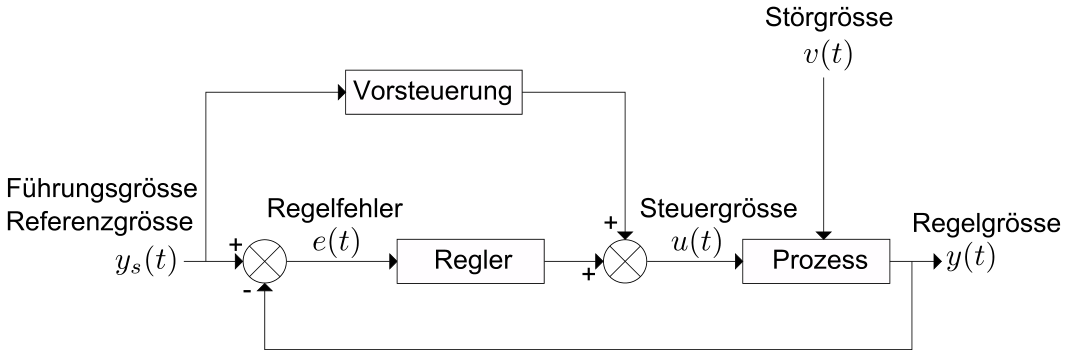
\includegraphics{images/paste-1.png}

}

\end{figure}

\hypertarget{minimalphasiges-system}{%
\subsection{Minimalphasiges System}\label{minimalphasiges-system}}

Liegen \ul{keine} Pole oder Nullstellen in der \ul{rechten Halbebene},
so spricht man von \textbf{minimalphasigen Systeme}. Amplituden- und
Phasengang stehen in einer direkten Beziehung zueinander. Es gilt
\textbf{nur bei minimalphasigen Systemen}:

\[
\angle{G}\approx\frac{\pi}{2}\cdot\frac{d{\log\lvert G\rvert}}{d{\log{\omega}}}
\]

Pro \(20\text{dB}\) Steigung oder Abfall beträgt die Phasenverschiebung
\(+90\degree\), respektive \(-90\degree\).

\hypertarget{fuxfchrungsverhalten}{%
\subsection{Führungsverhalten}\label{fuxfchrungsverhalten}}

\begin{figure}[H]

{\centering 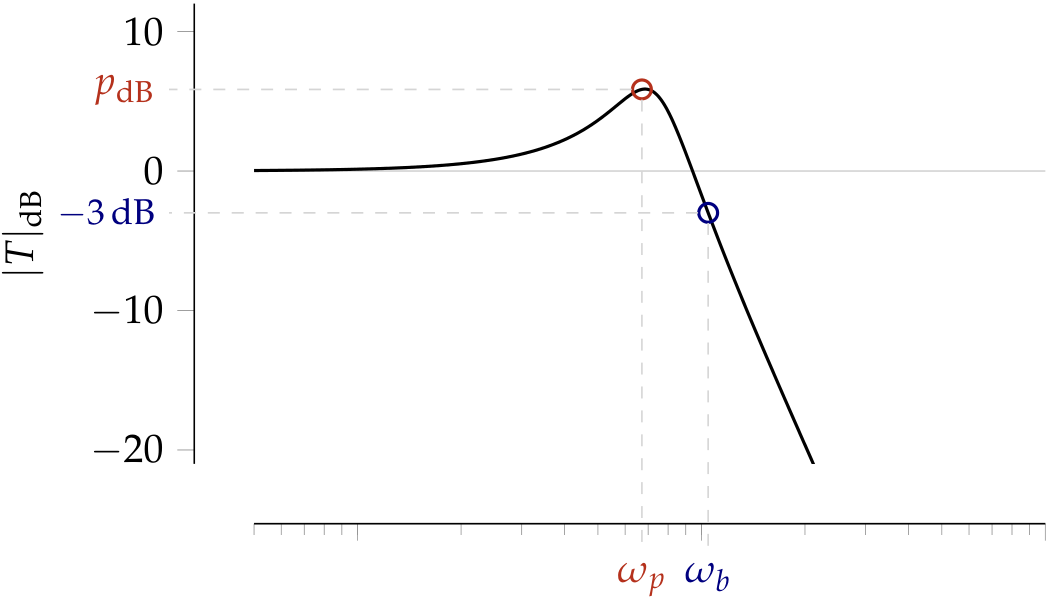
\includegraphics[width=6cm,height=\textheight]{images/paste-35.png}

}

\end{figure}

\[
G_{yr}=T=\frac{PC}{1+PC}\quad\text{und}\quad G_{ur}=CS=\frac{C}{1+PC}
\]

\hypertarget{merkmale}{%
\subsubsection{Merkmale}\label{merkmale}}

Das Führungsverhalten verfügt über vier Merkmale, welche für jedes
System betrachtet soll:

\begin{itemize}
\tightlist
\item
  \textbf{Stabilität}
\item
  \textbf{Statischer Fehler /} \textbf{stationäre Genauigkeit}
\item
  \textbf{Überschwingen}
\item
  \textbf{Schnelles Erreichen des stationären Wertes}
\end{itemize}

\textbf{Gutes Führungsverhalten}

\begin{figure}[H]

{\centering 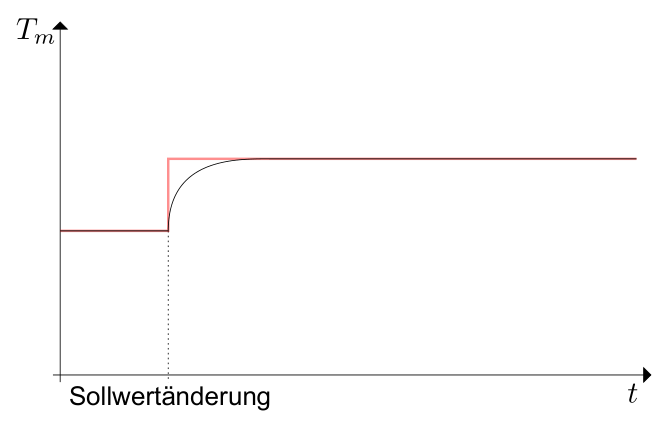
\includegraphics[width=6cm,height=\textheight]{images/fuhrungsverhalten/gutes_verhalten.png}

}

\end{figure}

\textbf{Instabilität}

\begin{figure}[H]

{\centering 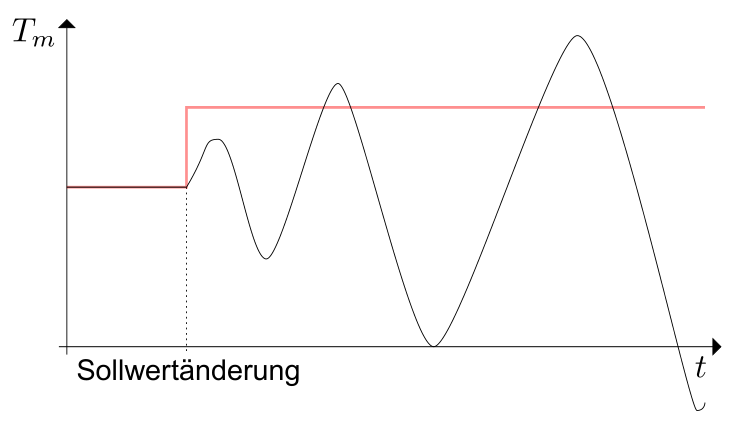
\includegraphics[width=6cm,height=\textheight]{images/fuhrungsverhalten/instabil.png}

}

\end{figure}

\textbf{Statischer Fehler /} \textbf{stationäre Ungenauigkeit}

\begin{figure}[H]

{\centering 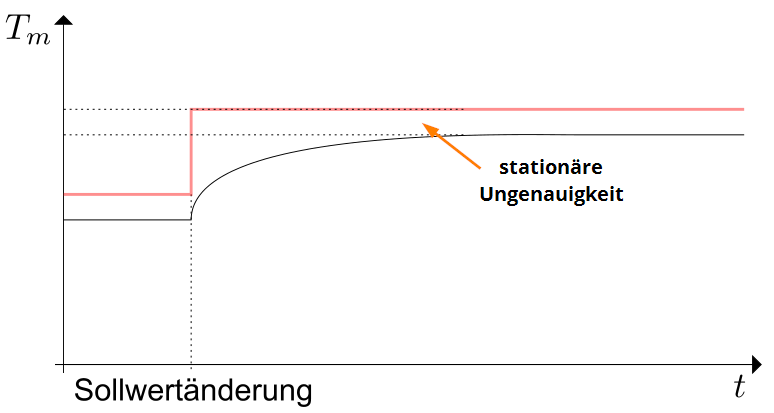
\includegraphics[width=6cm,height=\textheight]{images/fuhrungsverhalten/stationary.png}

}

\end{figure}

\textbf{Überschwingen}

\begin{figure}[H]

{\centering 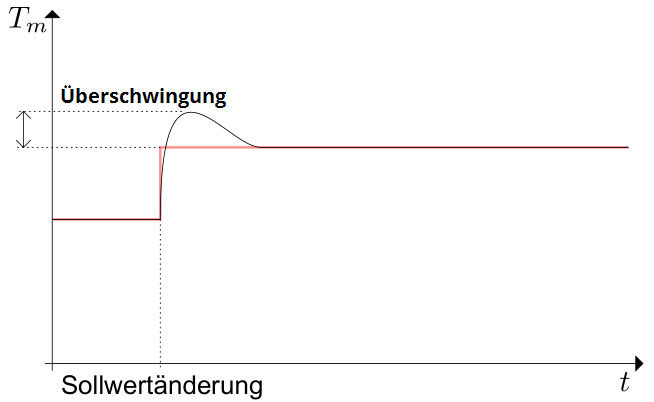
\includegraphics[width=6cm,height=\textheight]{images/fuhrungsverhalten/uberschwingung.png}

}

\end{figure}

\textbf{Langsames Erreichen des neuen stationären Wertes}

\begin{figure}[H]

{\centering 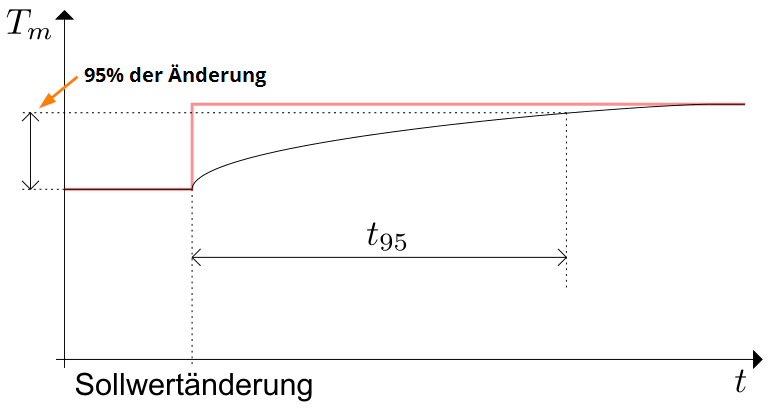
\includegraphics[width=6cm,height=\textheight]{images/fuhrungsverhalten/slow.png}

}

\end{figure}

\hypertarget{bleibende-fehler-bei-langsam-oder-nicht-uxe4ndernden-regelgruxf6ssen}{%
\subsubsection{Bleibende Fehler bei langsam oder nicht ändernden
Regelgrössen}\label{bleibende-fehler-bei-langsam-oder-nicht-uxe4ndernden-regelgruxf6ssen}}

Der bleibende Fehler bei sich langsam oder nicht ändernden
Führungssgrössen ergibt sich anhand des Verlaufs der
Übertragungsfunktion bei tiefen Frequenzen.

\[
G_{yr}\approx 1-e_0-e_1\cdot s-e_2\cdot s^2 - \cdots
\]

\[
e = e_0 \cdot r + e_1 \cdot \dot{r}+e_2\cdot \ddot{r}+\cdots
\]

\begin{figure}[H]

{\centering 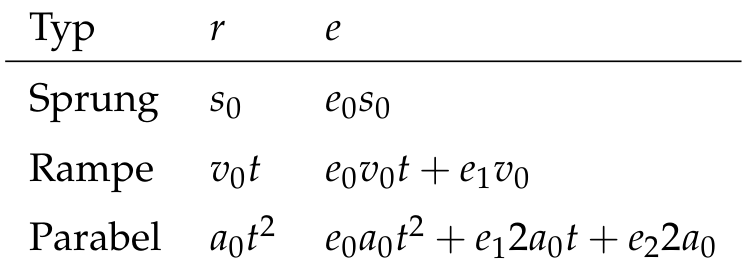
\includegraphics[width=5cm,height=1.8cm]{images/paste-37.png}

}

\end{figure}

\begin{tcolorbox}[enhanced jigsaw, opacitybacktitle=0.6, coltitle=black, arc=.35mm, title=\textcolor{quarto-callout-note-color}{\faInfo}\hspace{0.5em}{Stationärer Fehler}, opacityback=0, colframe=quarto-callout-note-color-frame, left=2mm, bottomtitle=1mm, toptitle=1mm, toprule=.15mm, breakable, leftrule=.75mm, colback=white, titlerule=0mm, bottomrule=.15mm, rightrule=.15mm, colbacktitle=quarto-callout-note-color!10!white]

Bei Rampe: \(e_0 = 0\qquad\) Bei Parabel \(e_0 = e_1 = 0\)

\end{tcolorbox}

\hypertarget{stuxf6rverhalten}{%
\subsection{Störverhalten}\label{stuxf6rverhalten}}

\[
G_{er}(s)=\frac{E(s)}{R(s)}
\]

\hypertarget{merkmale-1}{%
\subsubsection{Merkmale}\label{merkmale-1}}

Das Störverhlaten verfügt ebenfalls über vier Merkmale, welche für jedes
System betrachtet soll:

\begin{itemize}
\tightlist
\item
  \textbf{Stabilität}
\item
  \textbf{Statischer Fehler /} \textbf{stationäre Genauigkeit}
\item
  \textbf{Überschwingen}
\item
  \textbf{Schnelles Erreichen des stationären Wertes}.
\end{itemize}

\textbf{Gutes Störverhalten}

\begin{figure}[H]

{\centering 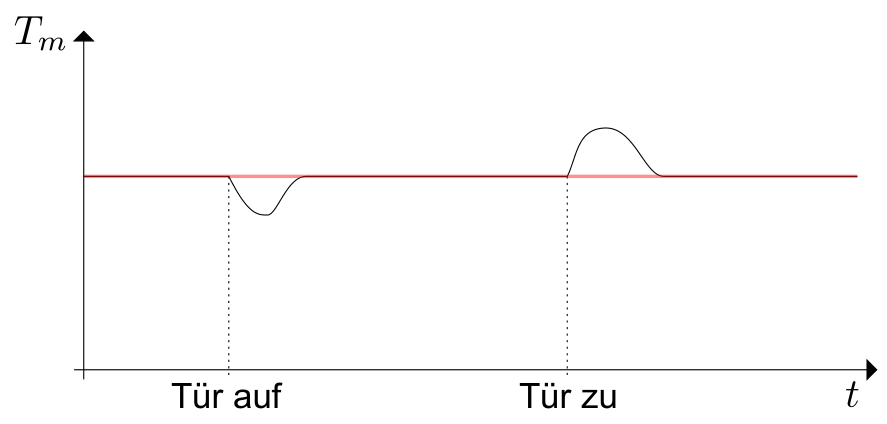
\includegraphics[width=6cm,height=\textheight]{images/storverhalten/gutes_verhalten.png}

}

\end{figure}

\textsuperscript{rot: Sollwert}

\textbf{Instabilität}

\begin{figure}[H]

{\centering 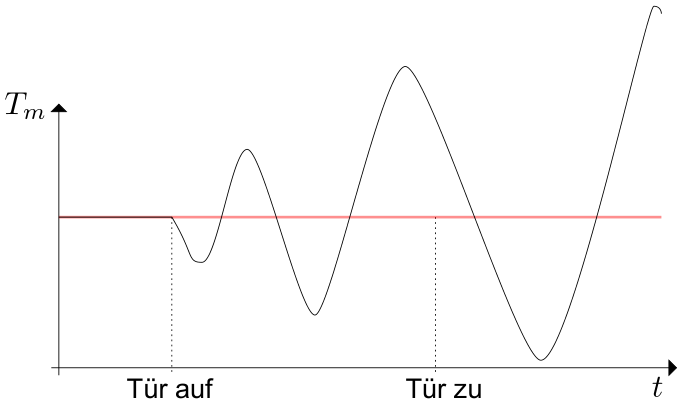
\includegraphics[width=6cm,height=\textheight]{images/storverhalten/storverhalten_stability.png}

}

\end{figure}

\textbf{Stationärer Fehler / Ungenauigkeit}

\begin{figure}[H]

{\centering 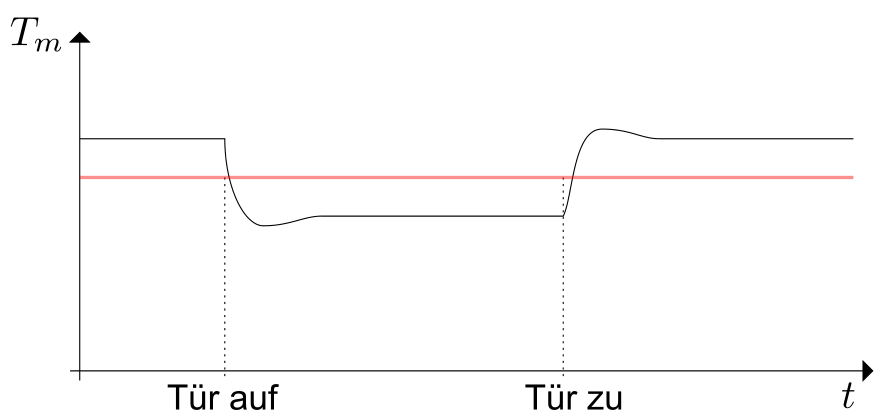
\includegraphics[width=6cm,height=\textheight]{images/storverhalten/storverhalten_stationary.png}

}

\end{figure}

\textbf{Überschwingen}

\begin{figure}[H]

{\centering 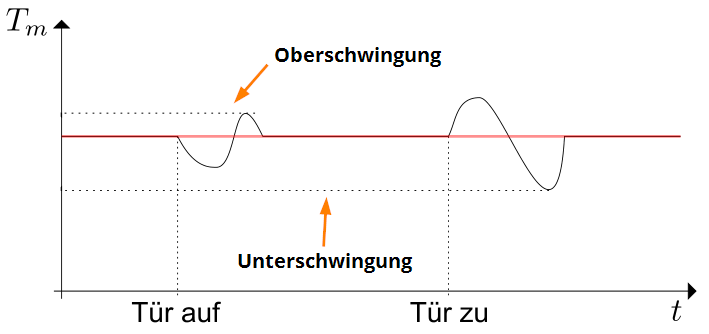
\includegraphics[width=6cm,height=\textheight]{images/storverhalten/uber_unterschwingung.png}

}

\end{figure}

\textbf{Langsames Erreichen des stationären Wertes}

\begin{figure}[H]

{\centering 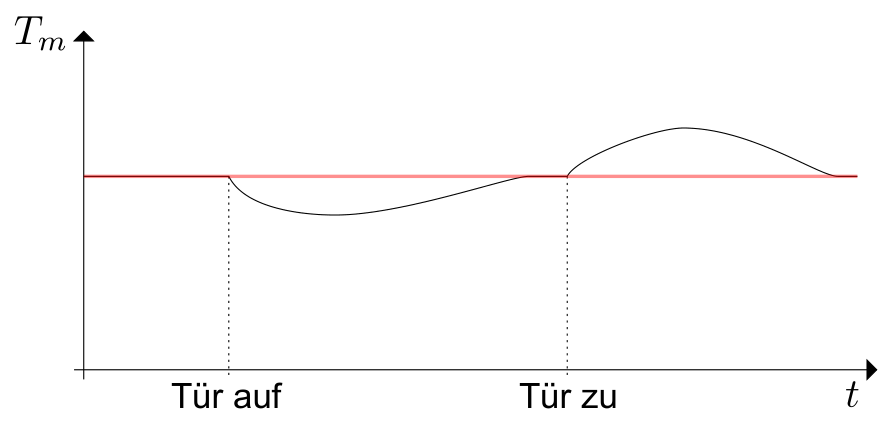
\includegraphics[width=6cm,height=\textheight]{images/storverhalten/slow.png}

}

\end{figure}

\hypertarget{darstellungsarten}{%
\section{Darstellungsarten}\label{darstellungsarten}}

\hypertarget{blockdiagrammalgebra}{%
\subsection{Blockdiagrammalgebra}\label{blockdiagrammalgebra}}

\hypertarget{verkettung}{%
\subsubsection{Verkettung}\label{verkettung}}

\begin{center}
\begin{tikzpicture}
    \node[box=0.8cm, minimum height=0.8cm] (sysG1) at (0,0) {$G_1$};
    \node[box=0.8cm, minimum height=0.8cm](sysG2) at (1.5,0) {$G_2$};
    \node[box=0.8cm, minimum height=0.8cm] (sysG12) at (0.75,-1) {$G_1G_2$};
    \node(start) at (-1.5,0) {};
    \node(end) at (3,0) {};
    \node(start2) at (-1,-1) {};
    \node(end2) at (2.5,-1) {};
    \draw[->]  (start2) edge node[above]{$u$} (sysG12);
    \draw[->]  (sysG12) edge node[above]{$y$} (end2);
    
    \draw[->]  (start) edge node[above]{$u$} (sysG1);
    \draw[->]  (sysG1) edge (sysG2);
    \draw[->]  (sysG2) edge node[above]{$y$}  (end);
    
\end{tikzpicture}
\end{center}

\[
y = G_2 ( G_1 \cdot u) = (G_1G_2)\cdot u
\]

\hypertarget{parallel}{%
\subsubsection{Parallel}\label{parallel}}

\begin{center}
\begin{tikzpicture}
    \node[box=0.8cm, minimum height=0.8cm] (sysG1) at (1,1.5) {$G_1$};
    \node[box=0.8cm, minimum height=0.8cm] (sysG2) at (1,0) {$G_2$};
    \node[box=0.8cm, minimum height=0.8cm] (sysG12) at (1,-1) {$G_1+G_2$};
    \node[dot] (dotStart) at (0,0.75) {};
    \node[sum] (sumEnd) at (2,0.75) {+};
    \node(start) at (-1.,0.75) {};
    \node(end) at (3,0.75) {};
    \node(start2) at (-1,-1) {};
    \node(end2) at (3,-1) {};
    \draw[->] (start2) edge node[above]{$u$} (sysG12);
    \draw[->] (sysG12) edge node[above]{$y$} (end2);
    
    \draw     (start) edge node[above]{$u$} (dotStart);
    \draw[->] (dotStart) |- (sysG1);
    \draw[->] (dotStart) |- (sysG2);
    \draw[->] (sysG1) -| (sumEnd);
    \draw[->] (sysG2) -| (sumEnd);
    \draw[->] (sumEnd) edge node[above]{$y$}  (end);
    
\end{tikzpicture}
\end{center}

\[
y = G_1\cdot u + G_1 \cdot u = (G_1 + G_2)\cdot u
\]

\hypertarget{ruxfcckkopplung}{%
\subsubsection{Rückkopplung}\label{ruxfcckkopplung}}

\begin{center}
\begin{tikzpicture}
    \node[sum] (sumStart) at (0,1) {$+$};
    \node[box=0.8cm, minimum height=0.8cm] (sysG) at (1.5,1) {$G$};
    \node[box=0.8cm, minimum height=0.8cm] (sysG12) at (1.25,-1) {$\frac{G}{1+G}$};
    \node(start) at (-1,1) {};
    \node(end) at (3.5,1) {};
    \node[dot] (endDot) at (2.5,1) {};
    \node(start2) at (-0.5,-1) {};
    \node(end2) at (3,-1) {};
    
    \draw[->]  (start2) edge node[above]{$r$} (sysG12);
    \draw[->]  (sysG12) edge node[above]{$y$} (end2);
    
    \draw[->]  (start) edge node[above]{$r$} (sumStart);
    \draw[->]  (sumStart) edge node[above]{$e$} (sysG);
    \draw      (sysG) edge (endDot);
    \draw[->]  (endDot) edge node[above]{$y$}  (end);
    
\draw[->] (endDot) -- (2.5,0) -- (0,0) -- node[above left]{$-$} (sumStart);
\end{tikzpicture}
\end{center}

\[
\begin{split}
y &= G\cdot e = G(r-y)\\
(1+G)\cdot y &= G\cdot r \\
y &= \underbrace{\frac{G}{1+G}}_{G_{yr}} \cdot r\\
\end{split}
\]

\hypertarget{regel-von-mason}{%
\subsubsection{Regel von Mason}\label{regel-von-mason}}

\[
G_{ij} = \frac{\sum_k P_k\cdot\Delta_k}{\Delta}
\]

\[
\begin{split}
P_k &= \text{Vorwärtspfad } k\\
\Delta = 1 &- \small{\Sigma\text{ aller Loops}} \\
           &+ \small{\Sigma\text{ aller Produkte 2er Loops, die sich nicht berühren}} \\
           &- \small{\Sigma\text{ aller Produkte 3er Loops, die sich nicht berühren}} \\
           &+ \cdots \\
\Delta_k = 1 &- \small{\Sigma\text{ aller Loops, die $P_k$ nicht berühren}} \\
             &+ \small{\Sigma\text{ aller Produkte 2er Loops, die $P_k$ \& sich nicht berühren}} \\
             &- \small{\Sigma\text{ aller Produkte 3er Loops, die $P_k$ \& sich nicht berühren}} \\
             &+ \cdots \\
\end{split}
\]

\ul{Beispiel}

\begin{figure}[H]

{\centering 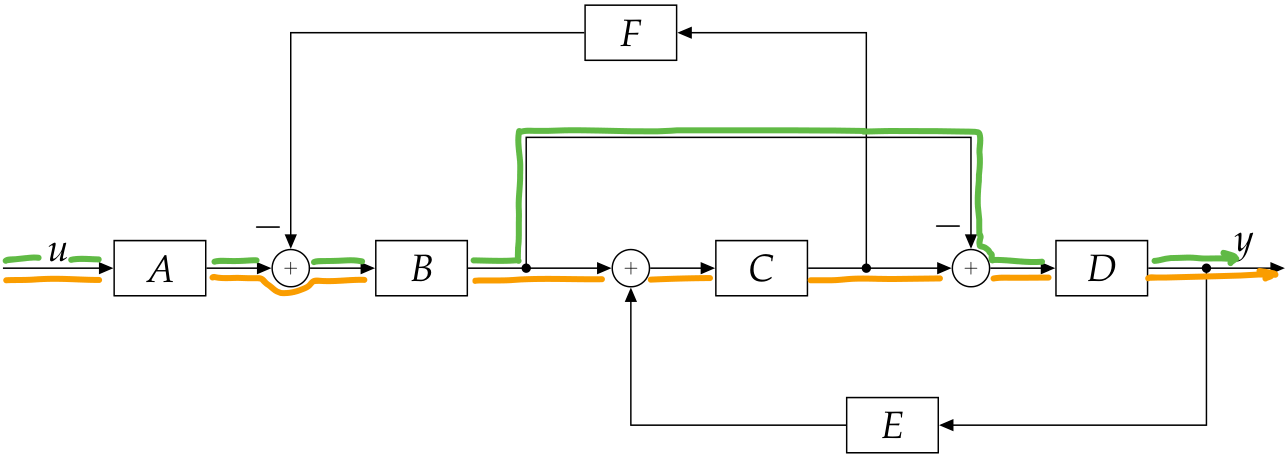
\includegraphics{images/paste-9.png}

}

\end{figure}

\begin{figure}[H]

{\centering 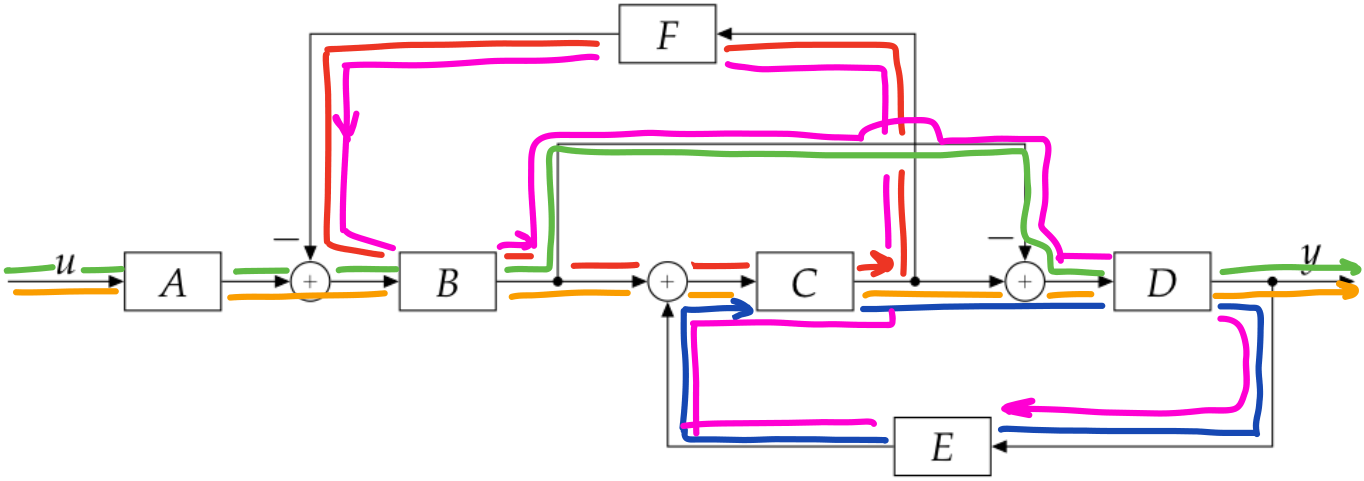
\includegraphics{images/paste-10.png}

}

\end{figure}

\(P_1 = ABCD \quad \Delta_1 = 1-0\quad P_2 = ABD \quad \Delta_2=1-0\)

\(\Delta=A-((-BCF)+CDE+((-B)(-D)(CEF))\)

\[
G_{uy}=\frac{ABD(1+C)}{A+BCF-CDE-BCDEF}
\]

\hypertarget{zustandraumdarstellung}{%
\subsection{Zustandraumdarstellung}\label{zustandraumdarstellung}}

Die Zustandsraumdarstellung erlaubt ein Einblick in das Verhalten eines
dynamischen Systems. Anhand eines \emph{Zeitdiagrammes} und
\emph{Phasenporträit} kann das System \emph{visualisiert} werden. Man
gibt Startkonditionen an und kann über das Phasenporträit den zeitlichen
Verlauf verfolgen.

\begin{figure}[H]

{\centering 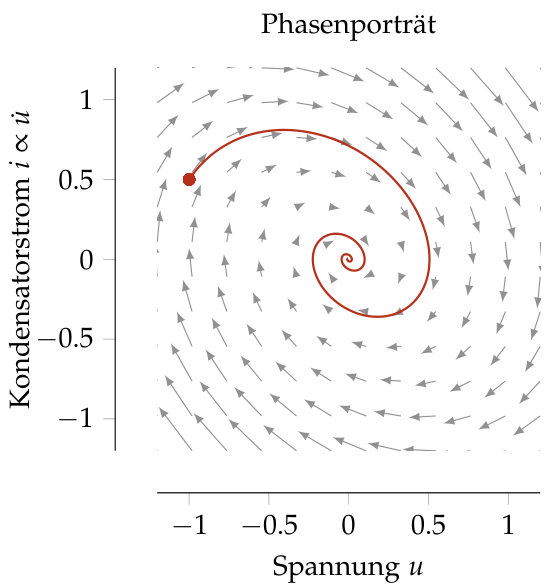
\includegraphics[width=5.7cm,height=\textheight]{images/state_space/quiver.png}

}

\end{figure}

\begin{figure}[H]

{\centering 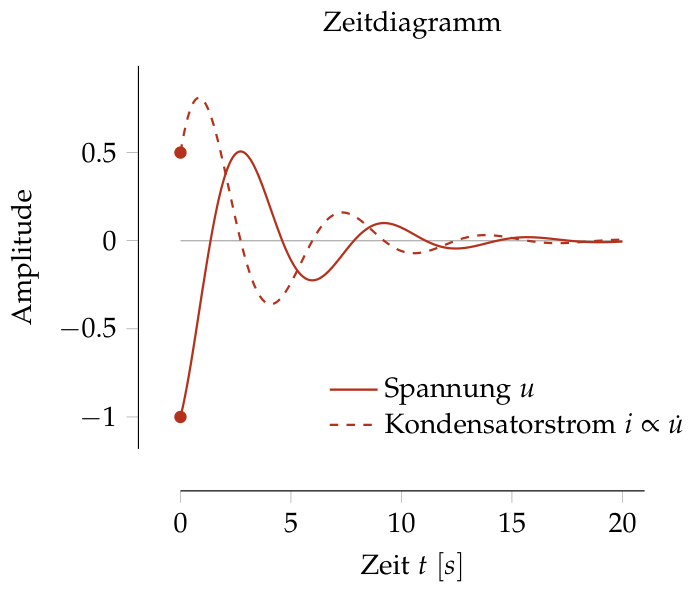
\includegraphics[width=6.3cm,height=\textheight]{images/state_space/time.png}

}

\end{figure}

\hypertarget{autonomes-zeitinvariantes-system}{%
\subsubsection{Autonomes, zeitinvariantes
System}\label{autonomes-zeitinvariantes-system}}

\begin{center}
  \begin{tikzpicture}
    \node[rectangle, draw=black, minimum width = 2cm] (a) at (0,0) {$\frac{dx}{dt} = f(x)$};
    \node (b) at (2,0) {};
    \draw[->] (a) -- node [above] {$x$} (b);
  \end{tikzpicture}
\end{center}

\[
\frac{dx}{dt}=f(x)
\]

Autonome Systeme berücksichtigen äusserliche Beeinflussungen \ul{nicht}
und sind ausschliesslich vom Anfangszustand abhängig.

\hypertarget{allgemeine-systeme}{%
\subsubsection{Allgemeine Systeme}\label{allgemeine-systeme}}

\begin{center}\begin{tikzpicture}

\node[rectangle, draw=black, minimum width = 2cm] (a) at (0,0) {
$
\begin{matrix}
\frac{dx}{dt} = f(x,u) \\
y=h(x,u)
\end{matrix}
$
};
\node (b) at (2,0) {};
\node (c) at (-2,0) {};

\draw[->] (a) -- node [above] {$y$} (b);
\draw[->] (c) -- node [above] {$u$} (a);

\end{tikzpicture}\end{center}

\[
\frac{dx}{dt}=f(x,u)\qquad y=h(x,u)
\]

\hypertarget{lineares-zustandsraummodell}{%
\subsubsection{Lineares
Zustandsraummodell}\label{lineares-zustandsraummodell}}

Viele der Systeme können an ein zeitinvariantes und lineares System
(LTI-System) angenähert werden.

\begin{center}\begin{tikzpicture}[scale=0.8]



\node (entry) at (-1,0) {$u$};
\node[rectangle, draw=black, minimum width=1cm] (integ) at (3.25,0) {$\int{dt}$};
\node[circle, draw=black] (circA) at (3.25,-1) {\textcolor{NavyBlue}{\textbf{A}}};
\node[circle, draw=black] (circB) at (1,0) {\textcolor{BurntOrange}{\textbf{B}}};
\node[sum] (add)   at (2,0) {+};
\node[sum] (add2) at (6.5,0) {+};
\node[circle, draw=black] (circC) at (5.5,0) {\textcolor{BrickRed}{\textbf{C}}};
\node[circle, draw=black] (circD) at (3.25,1) {\textcolor{OliveGreen}{\textbf{D}}};
\node [dot] (v2) at (4.5,0) {};
\node [dot] (v3) at (0,0) {};
\node (end) at (7.5,0) {$y$};


\draw [->] (integ) edge node [above]{$x$} (v2);
\draw [->] (v2) edge (circC);
\draw [->] (add) edge node[above]{$\dot{x}$} (integ);
\draw [->] (circB) edge (add);
\draw [->] (entry) edge (circB);
\draw [->] (circA) -| (add);
\draw [->] (v2) |- (circA);
\draw [->] (v3) |- (circD);
\draw [->] (circD) -| (add2);
\draw [->] (circC) -- (add2);
\draw [->] (add2) -- (end);
\end{tikzpicture}\end{center}

\[
\frac{dx}{dt}=\left(\begin{matrix} \dot{x}_1 \\ \dot{x}_2 \end{matrix}\right)=\textcolor{NavyBlue}{\mathbf{A}}x+\textcolor{BurntOrange}{\mathbf{B}}u \qquad y = \textcolor{BrickRed}{\mathbf{C}}x + \textcolor{OliveGreen}{\mathbf{D}}u
\]

\begin{conditions}
  A & beschreibt Dynamik \\
  B & beschreibt Steuereinfluss \\
  C & beschreibt Messung \\
  D & beschreibt Durchgriff
\end{conditions}

\hypertarget{uxfcbertragungsfunktion}{%
\subsubsection{Übertragungsfunktion}\label{uxfcbertragungsfunktion}}

Wird als Eingangssignal \(u\)

\[
u=\cos(\omega t)=\frac12(e^{+j\omega t}+e^{-j\omega t})
\]

gegeben, ergibt sich folgendes Ausgangssignal

\[
y(t)=\underbrace{C\textcolor{BrickRed}{e^{At}}(x(0)-(sI-A)^{-1}B)}_{\text{transient } y_t} + \underbrace{\overbrace{(C(sI-A)^{-1}B+D)}^{\text{Übertragungsfunktion}} e^{st}}_{\text{stationär } y_s}
\]

\begin{tcolorbox}[enhanced jigsaw, opacitybacktitle=0.6, coltitle=black, arc=.35mm, title=\textcolor{quarto-callout-note-color}{\faInfo}\hspace{0.5em}{Hinweis}, opacityback=0, colframe=quarto-callout-note-color-frame, left=2mm, bottomtitle=1mm, toptitle=1mm, toprule=.15mm, breakable, leftrule=.75mm, colback=white, titlerule=0mm, bottomrule=.15mm, rightrule=.15mm, colbacktitle=quarto-callout-note-color!10!white]

Ist \(A\) stabil, so geht der transiente Anteil \(y_t\) asymptotisch
gegen Null. Der stationäre Anteil bleibt übrig und entspricht der
Übertragungsfunktion.

\end{tcolorbox}

\hypertarget{dynamik}{%
\section{Dynamik}\label{dynamik}}

\hypertarget{luxf6sen-von-differential-gleichungen}{%
\subsection{Lösen von Differential
Gleichungen}\label{luxf6sen-von-differential-gleichungen}}

\begin{tcolorbox}[enhanced jigsaw, opacitybacktitle=0.6, coltitle=black, arc=.35mm, title=\textcolor{quarto-callout-important-color}{\faExclamation}\hspace{0.5em}{Lösung einer Differentialgleichung}, opacityback=0, colframe=quarto-callout-important-color-frame, left=2mm, bottomtitle=1mm, toptitle=1mm, toprule=.15mm, breakable, leftrule=.75mm, colback=white, titlerule=0mm, bottomrule=.15mm, rightrule=.15mm, colbacktitle=quarto-callout-important-color!10!white]

\[
x(t_0)=x_0\quad\frac{dx(t)}{dt}=F(x(t))
\]

\end{tcolorbox}

\hypertarget{gleichgewichtslage}{%
\subsection{Gleichgewichtslage}\label{gleichgewichtslage}}

Eine Gleichgewichtslage ist ein Zustand in dem das System \ul{stabil}
ist. Dies ist auch bekannt als \emph{stationäres} Verhalten und weist
\ul{keine} Veränderungen auf mit der Zeit.

\(x_e\) ist eine Gleichgewichtslage des dynamischen Systems
\(\frac{dx}{dt}=F(x)\) falls:

\[
F(x_e)=0 \rightarrow \frac{dx}{dt}\biggr\rvert_{x_e}=0
\]

\hypertarget{testfunktion-sprungantwort}{%
\subsection{Testfunktion
Sprungantwort}\label{testfunktion-sprungantwort}}

Anhand folgender Funktion kann die Sprungantwort eines Systems angegeben
werden.

\[
y(t)=Ce^{At}x(0)+\int^t_0Ce^{A(t-\tau)}Bu(\tau)d\tau+Du(t)
\]

Die Antwort setzt aus einem \emph{zeitabhängigen}~und einem
\emph{konstanten} Teil zusammen.

\[
y(t)=\underbrace{CA^{-1}e^{At}B}_{\text{zeitabhängig}}\underbrace{-CA^{-1}B+D}_{\text{konstant}}\qquad t>0
\]

Das System strebt gegen Wert wenn A \ul{asymptotisch stabil} ist
\(\rightarrow\) der \emph{zeitabhängige} Teil strebt, falls A
asymptotisch stabil ist, der Gleichtgewichtslage \(x=0\) zu. Der
\emph{konstante} Teil entspricht dem Wert bei \(\omega\rightarrow 0\)
und damit der \emph{Gleichspannungsverstärkung}.

\hypertarget{stabilituxe4t}{%
\section{Stabilität}\label{stabilituxe4t}}

\hypertarget{allgemein}{%
\subsection{Allgemein}\label{allgemein}}

Die Stabilität ist in drei Zustände eingeteilt.

\begin{itemize}
\tightlist
\item
  \textbf{stabil}, falls alle Zustände in der Nähe der
  Gleichgewichtslage \(x_e\) zu Lösungen führen.
\item
  \textbf{asymptotisch stabil}, falls alle Zustände in der Nähe von
  \(x_e\) nach langer Zeit (\(t \rightarrow \infty\)) in \(x_e\) enden.
\item
  \textbf{instabil}, falls der Zustand nie eine Gleichgewichtslage
  erreicht.
\end{itemize}

Stabilität ist im Allgemeinen eine \emph{lokale} Eigenschaft innerhalb
eines Bereiches des Zustandsraums!

\begin{tcolorbox}[enhanced jigsaw, opacitybacktitle=0.6, coltitle=black, arc=.35mm, title=\textcolor{quarto-callout-note-color}{\faInfo}\hspace{0.5em}{Beispiel}, opacityback=0, colframe=quarto-callout-note-color-frame, left=2mm, bottomtitle=1mm, toptitle=1mm, toprule=.15mm, breakable, leftrule=.75mm, colback=white, titlerule=0mm, bottomrule=.15mm, rightrule=.15mm, colbacktitle=quarto-callout-note-color!10!white]

Ein Pendel, welches die gesamte Rotationsachse (\(360\degree\),
rundherum) ausnützen kann, hat zwei Gleichgewichtslagen:

\begin{itemize}
\tightlist
\item
  \textbf{stabile} Position oben
\item
  \textbf{asymptotische stabile} Positionen, welche immer nach unten
  verlaufen.
\end{itemize}

\begin{figure}[H]

{\centering 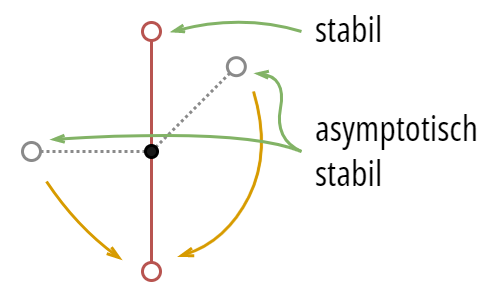
\includegraphics[width=6cm,height=\textheight]{images/dynamik/stationary_point.png}

}

\end{figure}

\end{tcolorbox}

\hypertarget{linearer-systeme}{%
\subsection{Linearer Systeme}\label{linearer-systeme}}

\begin{center}\begin{tikzpicture}

% x-Axis nodes
\node (xStart) at (-3,0) {};
\node (xEnd) at (3,0) {};

% y-Axis nodes
\node (yStart) at (0,-2.5) {};
\node (yEnd) at (0,2.5) {};

% Coloured Areas
\fill[green!50!orange!20] (-2.5,2) -- (-2.5,-2) -- (0,-2) -- (0,2) -- (-2.5,2);
\fill[red!50!orange!20] (2.5,2) -- (2.5,-2) -- (0,-2) -- (0,2) -- (2.5,2);

% Axis Arrows + Descriptions
\draw[-latex] (xStart) -- node[right = 2.75cm]{Re$(s)$} (xEnd);
\draw[-latex] (yStart) -- node[above = 2.3cm]{Im$(s)$} (yEnd);

% Area Descriptions
\node at (-1.25,1) {stabil};
\node at (1.25,1) {instabil};
\end{tikzpicture}\end{center}

Polstellen eines linearen Systems (\(\frac{dx}{dt}=Ax\) \& \(x(0)=x_0\))
können mit dem \emph{charakteristischen Polynoms} berechnet werden.

\begin{tcolorbox}[enhanced jigsaw, opacitybacktitle=0.6, coltitle=black, arc=.35mm, title=\textcolor{quarto-callout-important-color}{\faExclamation}\hspace{0.5em}{charakteristisches Polynom}, opacityback=0, colframe=quarto-callout-important-color-frame, left=2mm, bottomtitle=1mm, toptitle=1mm, toprule=.15mm, breakable, leftrule=.75mm, colback=white, titlerule=0mm, bottomrule=.15mm, rightrule=.15mm, colbacktitle=quarto-callout-important-color!10!white]

Die Nullstellen von \(\lambda\) werden mit der Dynamik-Matrix \(A\)
berechnet. Diese entsprechen dem Nennerpolynom \$C(sI-A)\^{}\{-1\}

\[
\lambda(A) := \{s \in \mathbb{C} :  \det(sI-A)=0\}
\]

\end{tcolorbox}

\begin{tcolorbox}[enhanced jigsaw, opacitybacktitle=0.6, coltitle=black, arc=.35mm, title=\textcolor{quarto-callout-caution-color}{\faFire}\hspace{0.5em}{Gültigkeit}, opacityback=0, colframe=quarto-callout-caution-color-frame, left=2mm, bottomtitle=1mm, toptitle=1mm, toprule=.15mm, breakable, leftrule=.75mm, colback=white, titlerule=0mm, bottomrule=.15mm, rightrule=.15mm, colbacktitle=quarto-callout-caution-color!10!white]

Stabilität linearer Systeme ist \ul{nur von} \(A\) \ul{abhängig}, nicht
vom Anfangswert \(x_0\). Dies gilt Global!

Ebenfalls sind stabile lineare Systeme \textbf{global} gültig.

\end{tcolorbox}

\hypertarget{linearisierung}{%
\subsubsection{Linearisierung}\label{linearisierung}}

Ist das linearisiterte System asymptotisch stabil, so ist das
nicht-lineare System in der \textbf{Umgebung der Gleichgewichtslage}
ebenfalls asymptotisch stabil.

\hypertarget{hurwitz-kriterium}{%
\subsection{Hurwitz-Kriterium}\label{hurwitz-kriterium}}

\begin{tcolorbox}[enhanced jigsaw, opacitybacktitle=0.6, coltitle=black, arc=.35mm, title=\textcolor{quarto-callout-important-color}{\faExclamation}\hspace{0.5em}{Wichtig}, opacityback=0, colframe=quarto-callout-important-color-frame, left=2mm, bottomtitle=1mm, toptitle=1mm, toprule=.15mm, breakable, leftrule=.75mm, colback=white, titlerule=0mm, bottomrule=.15mm, rightrule=.15mm, colbacktitle=quarto-callout-important-color!10!white]

\textbf{GESCHLOSSENER} KREIS VERWENDEN!

\end{tcolorbox}

\begin{tcolorbox}[enhanced jigsaw, opacitybacktitle=0.6, coltitle=black, arc=.35mm, title=\textcolor{quarto-callout-important-color}{\faExclamation}\hspace{0.5em}{Hurwitz-Kriterium}, opacityback=0, colframe=quarto-callout-important-color-frame, left=2mm, bottomtitle=1mm, toptitle=1mm, toprule=.15mm, breakable, leftrule=.75mm, colback=white, titlerule=0mm, bottomrule=.15mm, rightrule=.15mm, colbacktitle=quarto-callout-important-color!10!white]

Die Polstellen-Gleichung \(\lambda(s)\) mit \(a_0>0\) hat dann, und nur
dann, ausschliesslich Lösungen mit negativen reellen Teilen, falls alle
Unterdeterminante der Hurwitz-Matrix positiv sind:

\(\det H_n > 0\)

\end{tcolorbox}

\[
G_{yr}=\frac{\textcolor{NavyBlue}{P}\textcolor{BrickRed}{C}}{1+\textcolor{NavyBlue}{P}\textcolor{BrickRed}{C}}=\frac{\textcolor{NavyBlue}{n_P}\cdot\textcolor{BrickRed}{n_C}}{\textcolor{NavyBlue}{d_P}\cdot\textcolor{BrickRed}{d_C}+\textcolor{NavyBlue}{n_P}\cdot\textcolor{BrickRed}{n_C}}
\]

\begin{conditions}
  \textcolor{BrickRed}{n_C} & Zähler (\textit{numerator}) des Reglers $C$\\
  \textcolor{BrickRed}{d_C} & Nenner (\textit{divider}) des Reglers $C$\\
  \textcolor{NavyBlue}{n_P} & Zähler (\textit{numerator}) des Prozess $P$\\
  \textcolor{NavyBlue}{d_P} & Nenner (\textit{divider}) des Prozess $P$
\end{conditions}

\[
\lambda = {\textcolor{NavyBlue}{d_P}\cdot\textcolor{BrickRed}{d_C}+\textcolor{NavyBlue}{n_P}\cdot\textcolor{BrickRed}{n_C}} 
\]

\[
\lambda(s)=a_0\cdot s^n+a_1\cdot s^{n-1}+\cdots+a_{n-1}\cdot s+a_n
\]

\[
H=\begin{bmatrix}
  a_1 & a_3 & a_5 & a_7 & \cdots \\
  a_0 & a_2 & a_4 & a_6 & \cdots \\
  0   & a_1 & a_3 & a_5 & \cdots \\
  0   & a_0 & a_2 & a_4 & \cdots \\
  \vdots & \vdots & \vdots & \vdots & \ddots
\end{bmatrix} \in \mathbb{R}^{n\times n}
\]

\begin{tcolorbox}[enhanced jigsaw, opacitybacktitle=0.6, coltitle=black, arc=.35mm, title=\textcolor{quarto-callout-tip-color}{\faLightbulb}\hspace{0.5em}{Tipp}, opacityback=0, colframe=quarto-callout-tip-color-frame, left=2mm, bottomtitle=1mm, toptitle=1mm, toprule=.15mm, breakable, leftrule=.75mm, colback=white, titlerule=0mm, bottomrule=.15mm, rightrule=.15mm, colbacktitle=quarto-callout-tip-color!10!white]

\begin{itemize}
\tightlist
\item
  Bei \(n\leq 2\) genügt die Bedingung, dass alle Koeffizienten positiv
  sein müssen.
\item
  \(\det H_n = a_n \cdot \det H_{n-1}\) -- Wird nicht immer verwendet
  (nur bei Spalte Wert unten rechts, Rest der Spalte 0).
\item
  Fehlt ein Koeffizient oder ist dieser negativ, so ist die Bedingung
  nicht erfüllt
\end{itemize}

\[
s^3+2s^2+10\rightarrow\text{instabil, da } 0\cdot s
\]

\end{tcolorbox}

\begin{tcolorbox}[enhanced jigsaw, opacitybacktitle=0.6, coltitle=black, arc=.35mm, title=\textcolor{quarto-callout-caution-color}{\faFire}\hspace{0.5em}{Was mit Hurwitz nicht möglich ist}, opacityback=0, colframe=quarto-callout-caution-color-frame, left=2mm, bottomtitle=1mm, toptitle=1mm, toprule=.15mm, breakable, leftrule=.75mm, colback=white, titlerule=0mm, bottomrule=.15mm, rightrule=.15mm, colbacktitle=quarto-callout-caution-color!10!white]

Das Hurwitz-Kriterium beschreibt keine \emph{Robustheit} der Stabilität
und erlangt keine Einsicht, wie der Regler \(C=\frac{n_c}{d_c}\) gewählt
werden sollte.

\end{tcolorbox}

\ul{Beispiel}

\(\lambda = {8s^4}+{2}s^3+s^2+3s+2 = a_0s^4+a_1s^3+\cdots+a_4\)

\[
H = \begin{bmatrix}
2 & 3 & 0 \\
8 & 1 & 2 \\
0 & 2 & 3 \\
\end{bmatrix}
\]

\[
\begin{array}{l}
\det H_1 = 2 > 0\quad \textcolor{OliveGreen}{\checkmark}\\
\det H_2 = 2 - 24 = -22 > 0\quad \textcolor{BrickRed}{\large\times}\\
\end{array}
\]

\hypertarget{nyquist}{%
\subsection{Nyquist}\label{nyquist}}

Wenn \(L(s)=-1\), so kann eine stationäre Schwingung eingestellt werden!

\begin{center}
  \begin{tikzpicture}
    \node[box, minimum height=0.8cm, minimum width=0.8cm, inner sep=5pt] (procBox) at (0,2) {$-PC$};

    \node(endB) at (-2.5,2) {B};
    \node(startA) at (-1.5,2) {A};
    \draw[->] (startA) -- (procBox);
    \draw[->]  (procBox) -- (1,2) -- (1,1) -- (-3.5,1) -- (-3.5,2) -- (endB);
\end{tikzpicture}
\end{center}

\[
B=-P(s)C(s)\cdot A\quad \Rightarrow\quad \underline{P(s)C(s) = -1}
\]

\hypertarget{allgemein-variante-winkeluxe4nderung}{%
\subsubsection{Allgemein -- Variante
Winkeländerung}\label{allgemein-variante-winkeluxe4nderung}}

\begin{figure}[H]

{\centering 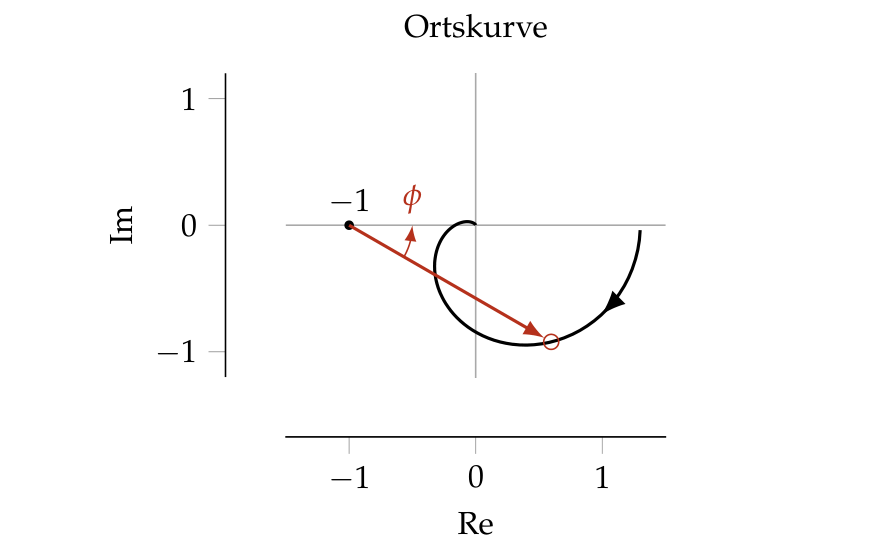
\includegraphics{images/paste-4.png}

}

\end{figure}

\[
\Delta\phi=a\frac{\pi}{2}+r\pi\,\hat{=}\,a\cdot90\degree+r\cdot180\degree
\]

\begin{conditions}
  a & Anzahl Pole \underline{auf} der $Im$-Achse\\
  r & Anzahl Pole \underline{rechts} der $Im$-Achse
\end{conditions}

Nur bei \(\Delta\phi\geq0\degree\) ist der \emph{geschlossene} Kreis
\textbf{stabil}.

\begin{tcolorbox}[enhanced jigsaw, opacitybacktitle=0.6, coltitle=black, arc=.35mm, title=\textcolor{quarto-callout-important-color}{\faExclamation}\hspace{0.5em}{Offen stabile Systeme}, opacityback=0, colframe=quarto-callout-important-color-frame, left=2mm, bottomtitle=1mm, toptitle=1mm, toprule=.15mm, breakable, leftrule=.75mm, colback=white, titlerule=0mm, bottomrule=.15mm, rightrule=.15mm, colbacktitle=quarto-callout-important-color!10!white]

Systeme, welche offen stabil sind, müssen der Bedinung \(\Delta\phi=0\)
genügen.

Das Kriterium ist ebenfalls anwendbar, wenn die Ortskurve experimentell
ermittelt wurde.

\end{tcolorbox}

\begin{tcolorbox}[enhanced jigsaw, opacitybacktitle=0.6, coltitle=black, arc=.35mm, title=\textcolor{quarto-callout-note-color}{\faInfo}\hspace{0.5em}{Totzeit}, opacityback=0, colframe=quarto-callout-note-color-frame, left=2mm, bottomtitle=1mm, toptitle=1mm, toprule=.15mm, breakable, leftrule=.75mm, colback=white, titlerule=0mm, bottomrule=.15mm, rightrule=.15mm, colbacktitle=quarto-callout-note-color!10!white]

Die Bedingung gilt auch für Systeme mit Totzeit

\end{tcolorbox}

\hypertarget{allgemein-variante-umluxe4ufe}{%
\subsubsection{Allgemein -- Variante
Umläufe}\label{allgemein-variante-umluxe4ufe}}

Das System \(G_{yr}\) ist stabil wenn \(P=U\)

\begin{conditions}
  P & Anzahl instabiler Polstellen von $L(s)$ \\
  U & Anzahl Umläufe der Nyquist-Kurve $L(j\omega)$ mit $\omega\in [-\infty,\infty]$ um den Punkt $(-1,0)$ im \underline{Gegenuhr}zeigersinn
\end{conditions}

\ul{Beispiel}

\[
L(s)=\frac{9(s+2)(s+4)}{(s-2)(s+3)(s-4)}
\]

\begin{figure}[H]

{\centering 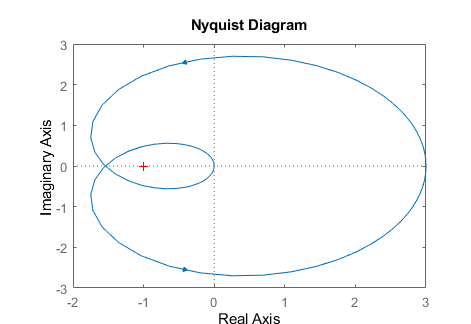
\includegraphics{images/paste-5.png}

}

\end{figure}

\(\rightarrow\ P=U=2: \textcolor{OliveGreen}{\text{stabil}}\)

\[ 
L(s)=\frac{18(s-1)(s+4)}{(s-2)(s+3)(s-4)}
\]

\begin{figure}[H]

{\centering 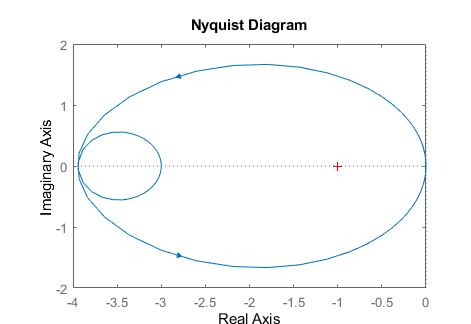
\includegraphics{images/paste-6.png}

}

\end{figure}

\(\rightarrow P=2,U=1:\textcolor{BrickRed}{\text{instabil}}\)

\hypertarget{einfach-variante-links-liegen}{%
\subsubsection{Einfach -- Variante Links
liegen}\label{einfach-variante-links-liegen}}

Für Systeme mit maximal zwei instabilen Polen im Ursprung (aber keinen
weiteren instabilen Polen) genügt die Bedingung, dass der Punkt
\((-1,0)\) \emph{links liegen gelassen} wird, wenn entlang der Ortskurve
\(\omega : 0 \rightarrow \infty\) verfahren wird.

\hypertarget{einfach-variante-umluxe4ufe}{%
\subsubsection{Einfach -- Variante
Umläufe}\label{einfach-variante-umluxe4ufe}}

Das System \(G_{yr}\) ist stabil, wenn die Nyquist Kurve \(L(j\omega)\)
mit \(\omega\in [0,\infty]\) den Punkt \((-1,0)\) \textbf{nicht}
umläuft.

\hypertarget{stabilituxe4tsreserve-robustheit}{%
\subsubsection{Stabilitätsreserve /
Robustheit}\label{stabilituxe4tsreserve-robustheit}}

\begin{figure}[H]

{\centering 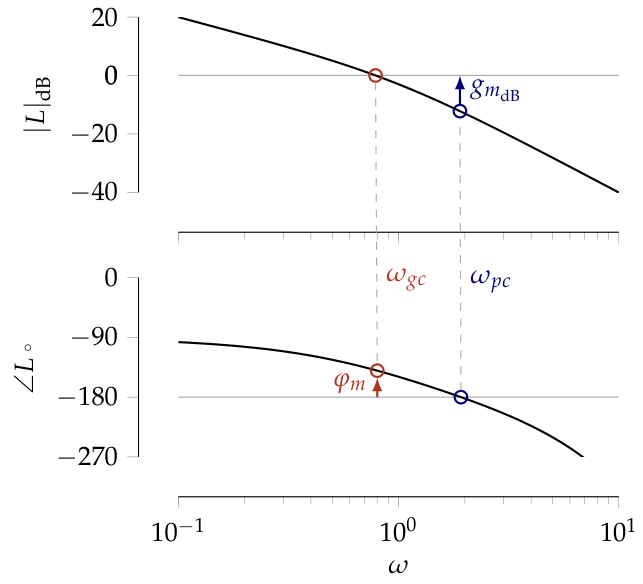
\includegraphics[width=6cm,height=\textheight]{images/paste-7.png}

}

\end{figure}

\begin{figure}[H]

{\centering 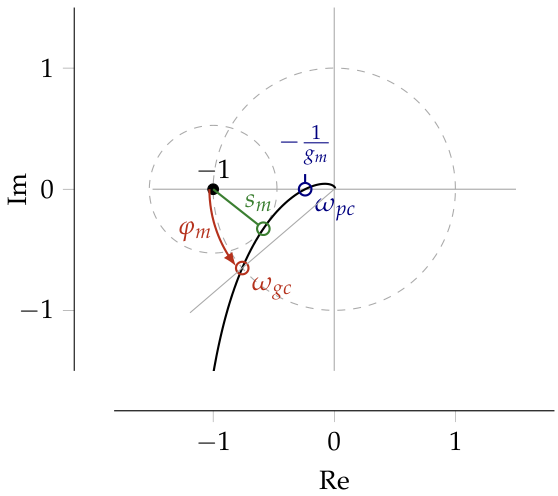
\includegraphics[width=6cm,height=\textheight]{images/paste-8.png}

}

\end{figure}

\hypertarget{phasenreserve-varphi_m}{%
\paragraph{\texorpdfstring{Phasenreserve
\(\varphi_m\)}{Phasenreserve \textbackslash varphi\_m}}\label{phasenreserve-varphi_m}}

Eintritt in den Einheitskreis \(\rightarrow\) \emph{gain crossover}

\[
\omega_{gc} : \lvert L(j\omega_{gc})\rvert = 1
\]

Abstand zu \(-1\) wird mit Phasenreserve \(\varphi_m\) ausgedrückt

\[
\varphi_m = 180\degree+\angle L(j\omega_{gc})
\]

\(\rightarrow\) kann im Bodediagramm abgelesen werden

\hypertarget{amplitudenreserve-g_m}{%
\paragraph{\texorpdfstring{Amplitudenreserve
\(g_m\)}{Amplitudenreserve g\_m}}\label{amplitudenreserve-g_m}}

Überschreiten der negativen \(Re\)-Achse \(\rightarrow\) \emph{phase
crossover}

\[
\omega_{pc} : \angle L(j\omega_{gc})= -180\degree
\]

Abstand zu \(-1\) wird durch die Amplitudenreserve \(g_m\) ausgedrückt.

\[
g_m = \frac1{\lvert L(j\omega_{pc})\rvert}
\]

Wird die Achse nicht überschritten, so ist \(g_m\rightarrow\infty\)

\(\rightarrow\) kann im Bodediagramm abgelesen werden

\hypertarget{stabilituxe4tsreserve-s_m}{%
\paragraph{\texorpdfstring{Stabilitätsreserve
\(s_m\)}{Stabilitätsreserve s\_m}}\label{stabilituxe4tsreserve-s_m}}

Kleinester Abstand zum Punkt \(-1\)

Der Wert kann von der Ortskurve abgelesen werden oder entspricht dem
Maximum der Sensitivitätsfunktion \(S\).

\[
\omega_{ms} = \underset{\omega}{\text{argmax}}\lvert S(j\omega)\rvert\qquad s_m = \frac1{\lvert S(j\omega_{ms})\rvert}=\frac1{g_{ms}}
\]

\begin{figure}[H]

{\centering 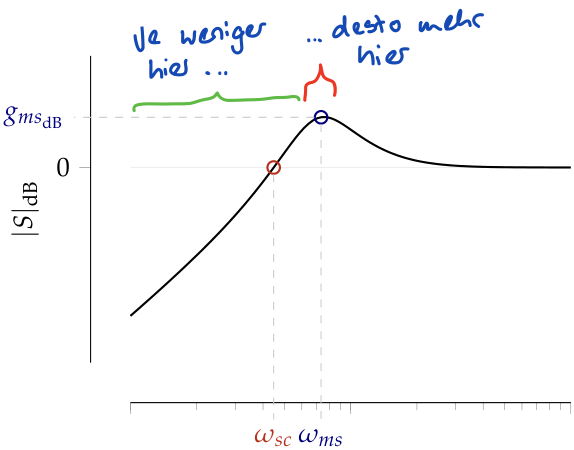
\includegraphics[width=6cm,height=\textheight]{images/paste-33.png}

}

\end{figure}

\begin{figure}[H]

{\centering 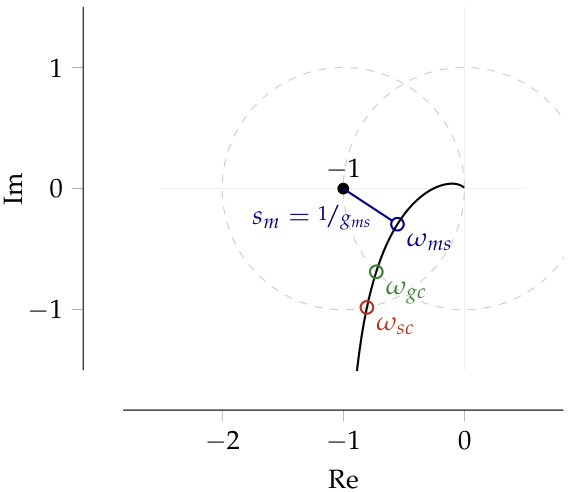
\includegraphics[width=6cm,height=\textheight]{images/paste-34.png}

}

\end{figure}

\begin{tcolorbox}[enhanced jigsaw, opacitybacktitle=0.6, coltitle=black, arc=.35mm, title=\textcolor{quarto-callout-note-color}{\faInfo}\hspace{0.5em}{Praxiswerte}, opacityback=0, colframe=quarto-callout-note-color-frame, left=2mm, bottomtitle=1mm, toptitle=1mm, toprule=.15mm, breakable, leftrule=.75mm, colback=white, titlerule=0mm, bottomrule=.15mm, rightrule=.15mm, colbacktitle=quarto-callout-note-color!10!white]

Folgende Werte dienen als \emph{Boilerplate} für die Reglerauslegung

\[
\begin{array}{l}
\varphi_m \approx 30\degree - 60\degree\\
g_m \approx 2-5 \\
s_m \approx 0.5 - 0.8 \\
\omega_{gc} \approx\frac1{\tau}: \tau\text{ von Sprungantwort}
\end{array}
\]

\end{tcolorbox}

\hypertarget{prozess}{%
\section{Prozess}\label{prozess}}

\begin{center}\begin{tikzpicture}
\node[box, minimum height=0.8cm, inner sep=5pt] (procBox) at (0,2) {Prozess $P$};

\node (start) at (-2,2) {};
\node (end) at (2,2) {};
\draw[->]  (start) edge (procBox);
\draw[->]  (procBox) edge (end);
\end{tikzpicture}\end{center}

\hypertarget{modellierung}{%
\subsection{Modellierung}\label{modellierung}}

\begin{tcolorbox}[enhanced jigsaw, opacitybacktitle=0.6, coltitle=black, arc=.35mm, title=\textcolor{quarto-callout-important-color}{\faExclamation}\hspace{0.5em}{Vereinfachung}, opacityback=0, colframe=quarto-callout-important-color-frame, left=2mm, bottomtitle=1mm, toptitle=1mm, toprule=.15mm, breakable, leftrule=.75mm, colback=white, titlerule=0mm, bottomrule=.15mm, rightrule=.15mm, colbacktitle=quarto-callout-important-color!10!white]

Modelle repräsentieren immer eine Vereinfachung des eigentlichen Systems
und fokusiert daher immer auf ein Teil des Systems.

\vspace{2mm}

\ul{Beispiel}: Die Modellierung des Tempomats konzentriert sich mehr auf
die Geschwindigkeit des Fahrzeugs als auf die Auswirkungen eines
Atombombeneinschlags auf das Fahrzeug.

\end{tcolorbox}

\hypertarget{identifikation}{%
\subsection{Identifikation}\label{identifikation}}

\underline{\footnotesize{...welche Klasse}} -- Ausgehend von einem
LTI-System sind der Grad von Zähler- und Nennerpolynom festzulegen.
Zudem sidn allfällige Totzeiten zu berücksichtigen.

\underline{\footnotesize{...welche Eingangssignale}} -- Das zu testende
System muss hinreichend mit einem Signal angeregt werden \(\rightarrow\)
Diracstösse, Sprungfunktionen, Rampen und harmonische Funktionen

\underline{\footnotesize{...was meint 'gleichwertig'}} -- Da Ein- \&
Ausgangsgrössen beobachtet werden, kann \(y\) des zu testenden Systems
und \(\hat{y}\) des zu vergleichenden Modell verglichen werden. Mit dem
resultierenden Fehler \(\epsilon = y - \hat{y}\) können Grenzen
festgelegt werden.

\underline{\footnotesize{...wie kann ein Modell gefunden werden}} --
Trial \& Error mit Sprungantwort und Bodediagramm.

\hypertarget{methode-der-kleinsten-quadrate}{%
\subsubsection{Methode der kleinsten
Quadrate}\label{methode-der-kleinsten-quadrate}}

Mit dieser Methode können Parameter anhand Messwerten bestummen werden.

\[
\begin{array}{r}
\underbrace{y[k]+a_1y[k-1]+a_2y[k-2]+\cdots+a_ny[k-n]}_{A(z^{-1})y}\\
= \underbrace{b_1u[k-1]+\cdots+b_nu[k-n]}_{B(z^{-1})u}
\end{array}
\]

\[
\beta^T=\begin{pmatrix}
a_1 & a_2 & \cdots & a_n & b_1 & b_2 & \cdots & b_n
\end{pmatrix}
\]

\[
\epsilon = A(z^{-1})y-B(z^{-1})u = \underbrace{y}_{Gemessen}-\underbrace{\Phi\beta}_{\text{Modell}}
\]

\[
y = \begin{pmatrix}
  y[n+1]\\
  y[n+2]\\
  \vdots\\
  y[n+N]
\end{pmatrix}
\]

\begin{figure}[H]

{\centering 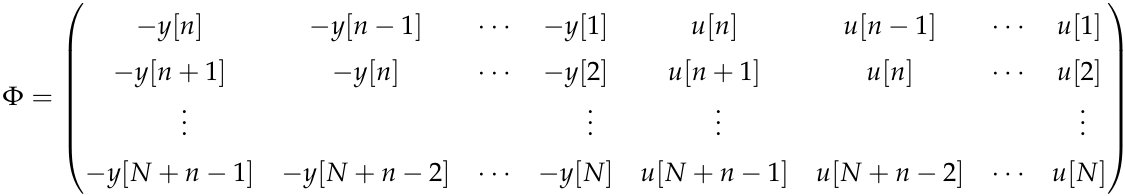
\includegraphics{images/paste-36.png}

}

\end{figure}

\[
\hat{\beta} = (\Phi^T\Phi)^{-1}\Phi^Ty
\]

\hypertarget{regelung}{%
\section{Regelung}\label{regelung}}

Feed\ul{back} Control

Ziel eines Reglers ist die Angleichung einer Regelgrösse \(y\) an eine
Führungsgrösse \(r\), sodass idealerweise \(y=r\).

\begin{center}
  \begin{tikzpicture}
    \fill[green!50!black!20] (-3,2) circle (0.2);
    \fill[blue!50!black!20] (2.5,2) circle (0.2);
    \node[above=1.5mm] at (2.5,2) {\textcolor{blue!50!black!90}{\textbf{1}}};
    \node[above=1.5mm] at (-3,2) {\textcolor{green!50!black!90}{\textbf{2}}};
    
    \node[box, minimum height=0.8cm, inner sep=5pt] (regBox) at (-1.5,2) {Regler $C$};
    \node[box, minimum height=0.8cm, inner sep=5pt] (procBox) at (1,2) {Prozess $P$};
    
    \node[sum] (sumPoint) at (-3,2) {+};
    \node (startNode) at (-4,2) {};
    \node[dot] (endDot) at (2.5,2) {};
    \node(endPoint) at (3.5,2) {};
    
    
    \draw[->] (startNode) -- node[above]{$r$} (sumPoint);
    \draw[->] (sumPoint) -- node[above]{$e$} (regBox);
    \draw[->] (regBox) -- node[above]{$u$} (procBox);
    \draw (procBox) -- (endDot);
    \draw[->] (endDot) -- node[above]{$y$} (endPoint);
    \draw[->] (endDot) -- (2.5,0.5) -- (-3,0.5) -- node[above left]{$-$} (sumPoint);
    \node (interferencePoint) at (1,3) {};
    \draw[->] (interferencePoint) -- node[above=2mm]{$v$} (procBox);
    
    \draw[->, orange!80!black!90, line width=1pt] (0.25,1.5) .. controls (1.25,0.5) and (-1.75,0.5) .. node[above]{\textbf{3}} (-0.75,1.5);
  
  \end{tikzpicture}
\end{center}

\begin{tcolorbox}[enhanced jigsaw, opacitybacktitle=0.6, coltitle=black, arc=.35mm, title=\textcolor{quarto-callout-tip-color}{\faLightbulb}\hspace{0.5em}{Merkmale einer Regelung}, opacityback=0, colframe=quarto-callout-tip-color-frame, left=2mm, bottomtitle=1mm, toptitle=1mm, toprule=.15mm, breakable, leftrule=.75mm, colback=white, titlerule=0mm, bottomrule=.15mm, rightrule=.15mm, colbacktitle=quarto-callout-tip-color!10!white]

Folgende Merkmale \textbf{muss} eine Regelung aufweisen, ansonsten ist
es keine Regelung.

\vspace*{2mm}

\hspace*{2mm}\textcolor{blue!50!black!90}{  \textbf{1}}. Erfassung
(Messen) der Regelgrösse\\
\hspace*{2mm}\textcolor{green!50!black!90}{  \textbf{2}}. Vergleich von
Regel- und Führungsgrösse\\
\hspace*{2mm}\textcolor{orange!80!black!90}{  \textbf{3}}. Geschlossener
Wirkungskreis

\end{tcolorbox}

\hypertarget{sensitivituxe4tsfunktionen}{%
\subsection{Sensitivitätsfunktionen}\label{sensitivituxe4tsfunktionen}}

\begin{center}
  \begin{tikzpicture}

    \node[box, minimum height=0.8cm, minimum width=0.8cm, inner sep=5pt] (regBox) at (-1.75,2) {$C$};
    \node[box, minimum height=0.8cm, minimum width=0.8cm, inner sep=5pt] (procBox) at (0.75,2) {$P$};

    \node[sum] (sumPoint) at (-3,2) {+};
    \node (startNode) at (-4,2) {};
    \node[dot] (endDot) at (2.5,2) {};
    \node(endPoint) at (3.5,2) {};
    \node[sum] (sumCP) at (-0.5,2) {+};
    \node[sum] (sumPY) at (2,2) {+};
    \node (intWPoint) at (2,3) {};
    \node (intVPoint) at (-0.5,3) {};


    \draw[->] (startNode) -- node[above]{$r$} (sumPoint);
    \draw[->] (sumPoint) -- node[above]{$e$} (regBox);
    \draw[->] (regBox) -- node[above]{$u$} (sumCP);
    \draw[->] (sumCP) -- node[above]{$\mu$} (procBox);
    \draw[->] (procBox) -- (sumPY);
    \draw     (sumPY) -- (endDot);
    \draw[->] (endDot) -- node[above]{$y$} (endPoint);
    \draw[->] (endDot) -- (2.5,1) -- (-3,1) -- node[above left]{$-$} (sumPoint);

    \draw[->] (intVPoint) -- node[above=3mm]{$v$} (sumCP);
    \draw[->] (intWPoint) -- node[above=3mm]{$w$} (sumPY);
  \end{tikzpicture}
\end{center}

\hypertarget{gang-of-four}{%
\subsubsection{`Gang of Four'}\label{gang-of-four}}

Das Verhalten der Regelung kann durch die folgenden vier
Sensitivitätsfunktionen beschrieben werden.

\underline{\footnotesize{Sensitivity Function}}

\[
G_{er} = S = \frac1{1+PC} 
\]

\begin{tcolorbox}[enhanced jigsaw, opacitybacktitle=0.6, coltitle=black, arc=.35mm, title=\textcolor{quarto-callout-note-color}{\faInfo}\hspace{0.5em}{Bedeutung}, opacityback=0, colframe=quarto-callout-note-color-frame, left=2mm, bottomtitle=1mm, toptitle=1mm, toprule=.15mm, breakable, leftrule=.75mm, colback=white, titlerule=0mm, bottomrule=.15mm, rightrule=.15mm, colbacktitle=quarto-callout-note-color!10!white]

Sensitivitäts-Übergangsfrequenz \(\omega_{sc}\) kennzeichnet den
Übergang von Dämpfung zur Verstärkung

\begin{center}\begin{tikzpicture}

\fill[green!50!orange!20]  (-3,1.5) rectangle (1,-1.5);
\fill[red!50!orange!20,draw=black, dashed]  (-1,0) node (circle_center) {} circle (1);

\node (circle_outer) at (-0.3115,0.7146) {};
\draw[->,gray]  (circle_center.center) -- node[above,scale=0.8]{$1$} (circle_outer.center);


% x-Axis 
\node (xStart) at (-3,0) {};
\node (xEnd) at (1,0) {};


% y-Axis
\node (yStart) at (0,-1.5) {};
\node (yEnd) at (0,1.5) {};


\draw[-latex] (xStart.center) -- node[above=0.2cm,right = 1.15cm,scale=0.8]{Re$(S)$} (xEnd.center);
\draw[-latex] (yStart.center) -- node[above = 1.3cm,right=1,scale=0.8]{Im$(S)$} (yEnd.center);
\end{tikzpicture}\end{center}

\[
\begin{array}{ll}
\lvert S(j\omega)\rvert < 1  & \textcolor{BrickRed}{\text{Dämpfung}} \\
\lvert S(j\omega)\rvert > 1  & \textcolor{OliveGreen}{\text{Verstärkung}}
\end{array}
\]

\end{tcolorbox}

\underline{\footnotesize{Load Sensitivity Function}}

\[
G_{vy} = PS = \frac1{1+PC} 
\]

\underline{\footnotesize{Complementary Sensitivity Function}}

\[
G_{yr} = T = \frac1{1+PC} \stackrel{!}{=} \underline{1}
\]

\underline{\footnotesize{Noise Sensitivity Function}}

\[
G_{ur} = CS = \frac{C}{1+PC} 
\]

\hypertarget{anforderungen}{%
\subsection{Anforderungen}\label{anforderungen}}

\hypertarget{stabilituxe4t-1}{%
\subsubsection{Stabilität}\label{stabilituxe4t-1}}

\begin{figure}[H]

{\centering 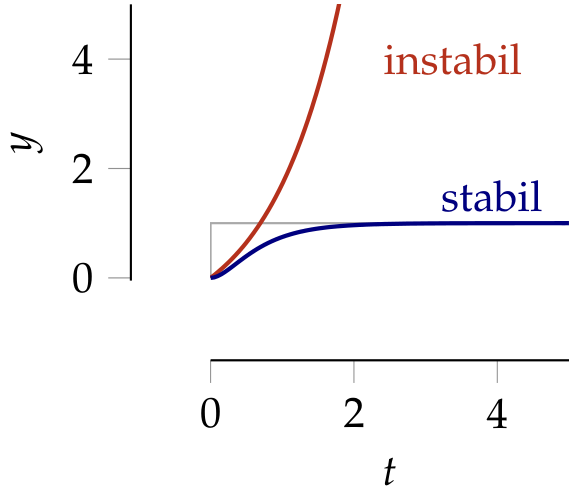
\includegraphics[width=4cm,height=3.5cm]{images/paste-11.png}

}

\end{figure}

\begin{itemize}
\tightlist
\item
  binäres Kriterium und \ul{zwingend zu erfüllen}
\item
  Für lineare Systeme gilt dies \textbf{global}, egal welcher AP
\item
  Die Stabilität kann anhand des Polnullstellendiagramms beurteilt und
  mit Hurwitz \& Nyquist untersucht werden
\end{itemize}

\hypertarget{stationuxe4re-genauigkeit}{%
\subsubsection{Stationäre Genauigkeit}\label{stationuxe4re-genauigkeit}}

\begin{figure}[H]

{\centering 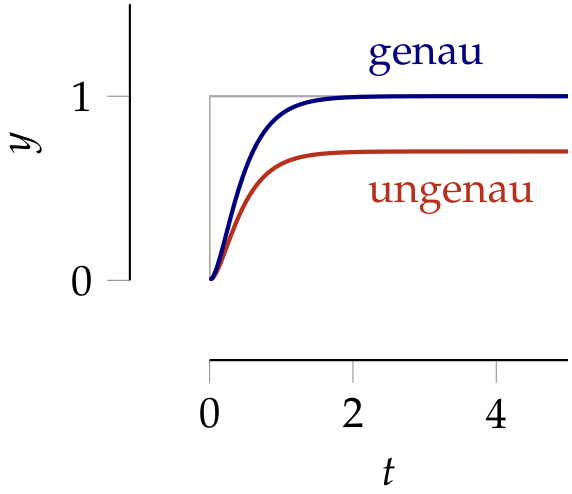
\includegraphics[width=4cm,height=3.5cm]{images/paste-12.png}

}

\end{figure}

\begin{itemize}
\tightlist
\item
  Beschreibt bleibender Fehler, nach Abklingung der transienten Vorgänge
\item
  Gutes Mass ist stationärer Regelfehler \(e\)
\end{itemize}

\[
e = \frac1{1+PC}r+\frac{-P}{1+PC}v+\frac{-1}{1+PC}w
\]

\[
e_{stationär}=\small\frac{1}{1+PC}\biggr\rvert_{s=0}\cdot r_0+\small\frac{-P}{1+PC}\biggr\rvert_{s=0}\cdot v_0+\small\frac{-1}{1+PC}\biggr\rvert_{s=0}\cdot w_0
\]

\hypertarget{schnelligkeit}{%
\subsubsection{Schnelligkeit}\label{schnelligkeit}}

\begin{figure}[H]

{\centering 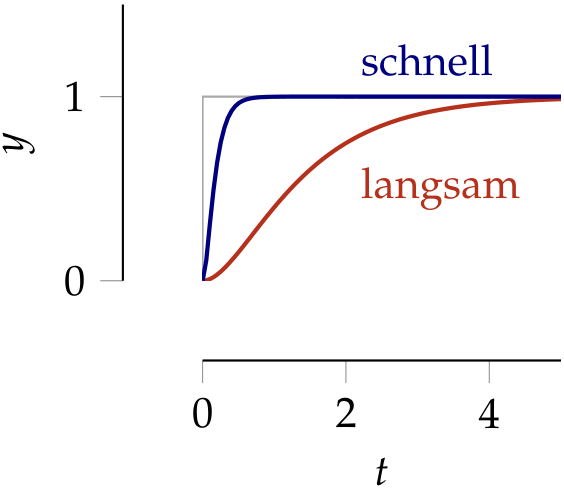
\includegraphics[width=4cm,height=\textheight]{images/paste-13.png}

}

\end{figure}

\begin{itemize}
\item
  Für Charakterisierung des dynamischen Verhaltens wird
  \textbf{Gesamtregelkreis} betrachtet in Bezug auf Führungsgrösse

  \[
  y = \frac{PC}{1+PC}r
  \]
\item
  Als Kriterium dient die Grenzfrequenz \(\omega_g \rightarrow\)
  Beschreibt ab wann das Verhalten deutlich degradiert
  (\(\omega_g<\omega\))

  \[
  \omega_g: \lvert L(s) \rvert_{s=j\omega_g}\approx 1
  \]
\end{itemize}

\begin{figure}[H]

{\centering 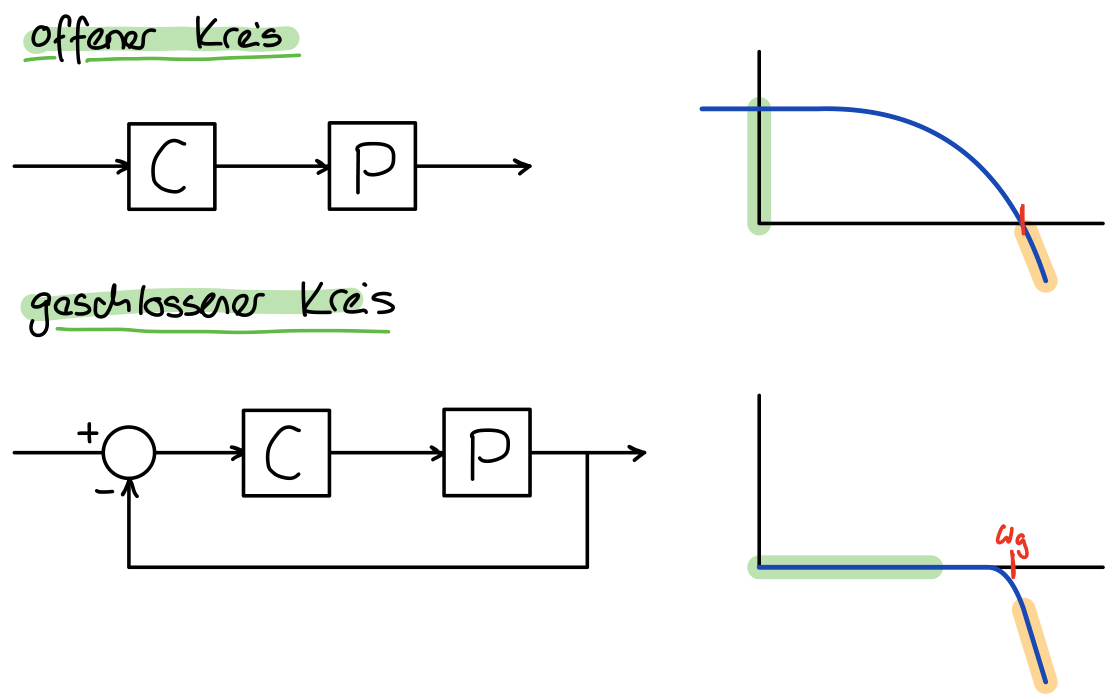
\includegraphics{images/paste-15.png}

}

\end{figure}

\hypertarget{duxe4mpfung}{%
\subsubsection{Dämpfung}\label{duxe4mpfung}}

\begin{figure}[H]

{\centering 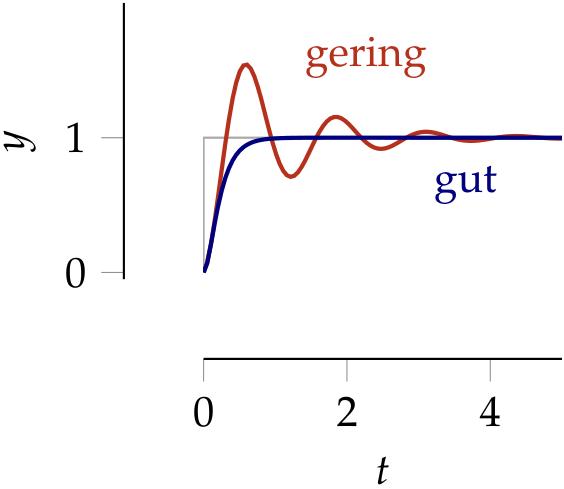
\includegraphics[width=4cm,height=\textheight]{images/paste-14.png}

}

\end{figure}

\begin{itemize}
\tightlist
\item
  Unterdrückung von schwingenden Signalteilen, welche Anzeichen von
  Instabilität sind
\item
  Gutes Mass ist die Phasenlage im Bereich von \(\omega_g\)
\end{itemize}

\hypertarget{eigenschaften}{%
\subsection{Eigenschaften}\label{eigenschaften}}

\hypertarget{robustheit}{%
\subsubsection{Robustheit}\label{robustheit}}

\emph{Robustheit} bezeichnet die Fähigkeit eines Systems, Veränderungen
ohne Anpassung seiner anfänglich stabilen Struktur standzuhalten.

Robustheit gegenüber Unsicherheit \(\rightarrow\) Standhaltung gegenüber
Störungen

\hypertarget{dynamik-1}{%
\subsubsection{Dynamik}\label{dynamik-1}}

Die \emph{Dynamik} eines Systems kann durch eine Regelung beeinflusst
und verändert werden.

\begin{itemize}
\tightlist
\item
  Instabile Systeme \(\rightarrow\) stabil
\item
  Träges System \(\rightarrow\) schnell
\item
  Abdriftende System \(\rightarrow\) konstant\emph{.}
\end{itemize}

\begin{tcolorbox}[enhanced jigsaw, opacitybacktitle=0.6, coltitle=black, arc=.35mm, title=\textcolor{quarto-callout-caution-color}{\faFire}\hspace{0.5em}{Abhängigkeit}, opacityback=0, colframe=quarto-callout-caution-color-frame, left=2mm, bottomtitle=1mm, toptitle=1mm, toprule=.15mm, breakable, leftrule=.75mm, colback=white, titlerule=0mm, bottomrule=.15mm, rightrule=.15mm, colbacktitle=quarto-callout-caution-color!10!white]

Viele Systemeigenschaften sind \ul{nicht} unabhängig voneinander. Sie
unterliegen von Natur aus bestimmten Beschränkungen

\begin{itemize}
\tightlist
\item
  Stabiles Flugverhalten \(\rightarrow\) keine hohe Manövrierbarkeit
\end{itemize}

\textcolor{BurntOrange}{!!} \ul{Regelungen} können \ul{helfen}, diese
\ul{Abhängigkeiten teilweise aufzuheben}!

\end{tcolorbox}

\begin{tcolorbox}[enhanced jigsaw, opacitybacktitle=0.6, coltitle=black, arc=.35mm, title=\textcolor{quarto-callout-warning-color}{\faExclamationTriangle}\hspace{0.5em}{Safety Critical}, opacityback=0, colframe=quarto-callout-warning-color-frame, left=2mm, bottomtitle=1mm, toptitle=1mm, toprule=.15mm, breakable, leftrule=.75mm, colback=white, titlerule=0mm, bottomrule=.15mm, rightrule=.15mm, colbacktitle=quarto-callout-warning-color!10!white]

Werden instabile Systeme mittels Regelung stabilisiert, so wird die
Regelung kritisch für die Sicherheit des Systems.

\end{tcolorbox}

\hypertarget{modularituxe4t}{%
\subsubsection{Modularität}\label{modularituxe4t}}

In einem modularen System sind die einzelnen Module möglichst unabhängig
voneinander \(\rightarrow\) Module können einfach ersetzt oder erweitert
werden.

\begin{itemize}
\tightlist
\item
  Wohldefinierte Ein-/Ausgänge, Beziehungen dazwischen \(\rightarrow\)
  Verhalten unabhängig von äusseren Umständen \(\rightarrow\) ebenfalls
  Ziel von Regler
\end{itemize}

Mittels Regelulng lassen sich Komponenten unabhängiger und damit
zusammengesetzte Systeme Modularer machen.

\hypertarget{genauigkeit}{%
\subsubsection{Genauigkeit}\label{genauigkeit}}

Mit Regelung können unerwünschte Störeinflüsse ausgeglichen werden
\(\rightarrow\) Verbessert Genauigkeit und Auflösung (z.B. bei
Sensoren).

\begin{tcolorbox}[enhanced jigsaw, opacitybacktitle=0.6, coltitle=black, arc=.35mm, title=\textcolor{quarto-callout-note-color}{\faInfo}\hspace{0.5em}{Anwendungen}, opacityback=0, colframe=quarto-callout-note-color-frame, left=2mm, bottomtitle=1mm, toptitle=1mm, toprule=.15mm, breakable, leftrule=.75mm, colback=white, titlerule=0mm, bottomrule=.15mm, rightrule=.15mm, colbacktitle=quarto-callout-note-color!10!white]

Ein Konzept einer hohen Genauigkeit ist, mittels Regelung wird ein
bestimmten und wohldefinierten Arbeitspunkt ausgeregelt und dabei
aufgewendete Stellgrösse als Messgrösse des Sensors interpretiert dies.

\ul{Beispiel}: Seismographgen, sehr präzise Waagen

\end{tcolorbox}

\hypertarget{herauserforderungen}{%
\subsubsection{Herauserforderungen}\label{herauserforderungen}}

Regelungen bringen viele Vorteile, aber auch einige Nachteile:

\textbf{Gefahr der Instabilität} -- Auch geregelte Systeme haben einen
Kipppunkt, wo die Mitkopplung dominant wird und zur Instabilität führt.
Ziel einer Regelung ist das System unter allen Umständen stabil zu
halten (nicht nur unter Normalbedingung sondern auch unter allen
Störeinflüssen \(\rightarrow\) anspruchsvoll).

\ul{Beispiel}: Mikrophonverstärkung bei Beschallungsanlage zu weit
aufgedreht \(\rightarrow\) pfeifen

\textbf{Messfehler} -- Jede Regelgrösse wird messtechnisch verfasst
\(\rightarrow\) verbundene Messfehler gehen in Systemverhalten ein
(betrifft statische Fehler, dynamische Fehler, wie Rauschen)

\textbf{Komplexität} -- Die Implementation eines Regelsystems bei hoher
Komplexität wird anspruchsvoller und mit entsprechendem Aufwand
verbunden.

\hypertarget{steuerung}{%
\subsection{Steuerung}\label{steuerung}}

Feed\ul{forward} Control

\begin{figure}[H]

{\centering 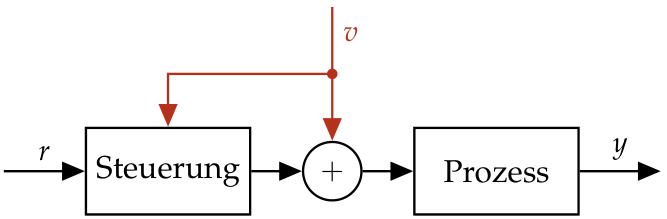
\includegraphics[width=8cm,height=\textheight]{images/basics/control.png}

}

\end{figure}

\hypertarget{p-regler}{%
\subsection{P-Regler}\label{p-regler}}

\[
C(s) = k_p \qquad u = k_p\cdot e
\]

\begin{tcolorbox}[enhanced jigsaw, opacitybacktitle=0.6, coltitle=black, arc=.35mm, title=\textcolor{quarto-callout-warning-color}{\faExclamationTriangle}\hspace{0.5em}{Achtung}, opacityback=0, colframe=quarto-callout-warning-color-frame, left=2mm, bottomtitle=1mm, toptitle=1mm, toprule=.15mm, breakable, leftrule=.75mm, colback=white, titlerule=0mm, bottomrule=.15mm, rightrule=.15mm, colbacktitle=quarto-callout-warning-color!10!white]

\(e=0\) ist mit einem P-Regler nicht möglich. Unter Annahme eines
stabilen Regelkreises:

\[
G_{er}=\frac{1}{1+P\cdot C}=\frac{1}{1+P\cdot k_p}
\]

entsteht ein bleibender Fehler von:

\[
G_{er}(0)=\frac{1}{1+P(0)\cdot C(0)}=\frac{1}{1+P(0)\cdot k_p}
\]

Dies kann mit einer Vorsteuerung korrigiert werden, was aber
Störeinflüsse \ul{nicht} ausschliesst:

\[
u(t) = k_p\cdot e(t) + u_{ff} = k_p\cdot e(t)+\frac{r}{P(0)}
\]

Besser ist ein PI-Regler

\end{tcolorbox}

\hypertarget{pi-regler}{%
\subsection{PI-Regler}\label{pi-regler}}

\[
C_{PI}=k_p\cdot\left(1+\frac1{T_i s}\right)\qquad u = k_i\cdot\int_0^t e(\tau)\ {\text{d}\tau}
\]

\hypertarget{pd-regler}{%
\subsection{PD-Regler}\label{pd-regler}}

\[
C_{PD} = k_p\cdot (1 + T_d\cdot s)\qquad u = k_d\frac{de}{dt}
\]

\hypertarget{filter-d-anteil}{%
\subsubsection{Filter D-Anteil}\label{filter-d-anteil}}

Hochfrequente Änderungen (z.B. Sprungantworten) führt zu hohem D-Anteil
\(\rightarrow\) Erweiterung TP-Filter

\begin{center}
  \begin{tikzpicture}

    \node[box, minimum height=0.8cm, minimum width=0.8cm, inner sep=5pt] (procP) at (-2,0) {$k_d$};
    \node[box, minimum height=0.8cm, minimum width=0.8cm, inner sep=5pt] (procTP) at (0,0) {$\small\frac{s}{1+sT_d}$};
    
    
\node(start) at (-3.25,0) {$e$};
\node(end) at (1.5,0) {$u$};
\draw[->]   (start) edge (procP);
\draw[->]  (procP) edge (procTP);
\draw[->]  (procTP) edge (end);


\end{tikzpicture}
\end{center}

Für tiefe Frequenzen (\(\lvert s\rvert\ll\frac1{T_d}\)) wird
\(G_{ue}\approx k_p T_ds\) und hohe Frequenzen wird
\(G_{ue}\approx k_p\) (limitiert durch \(k_p\))

\[
C_{D}(s)= k_p\frac{T_d\cdot s}{1+s\cdot T_d} = \frac{\overbrace{k_d\cdot s}^{\text{D-Anteil}}}{\underbrace{1+s\cdot T_d}_{\text{Filter}}}
\]

\hypertarget{pid-regler}{%
\subsection{PID-Regler}\label{pid-regler}}

\begin{figure}[H]

{\centering 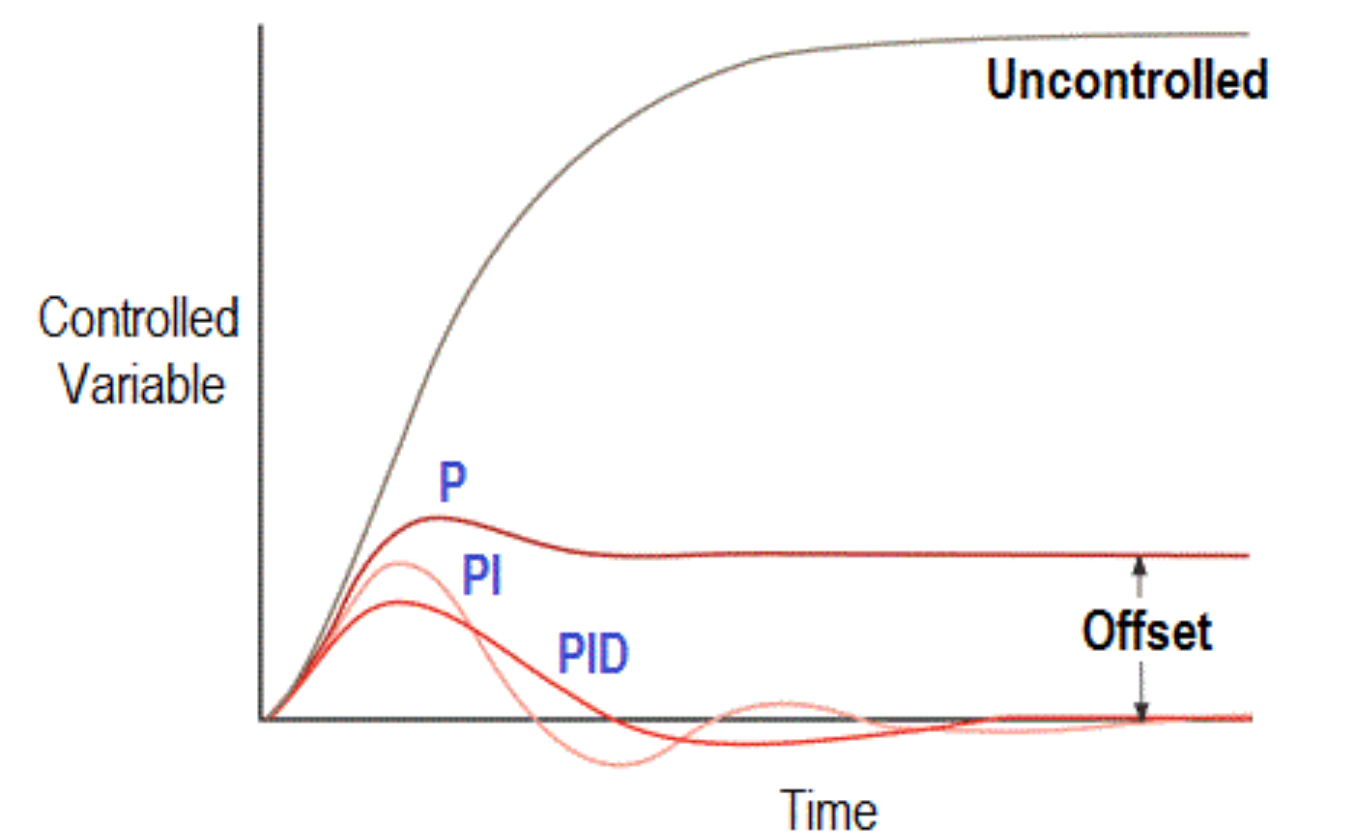
\includegraphics[width=7cm,height=\textheight]{images/pid_regler/PID-Controller-Graph-1906105412.png}

}

\end{figure}

\begin{figure}[H]

{\centering 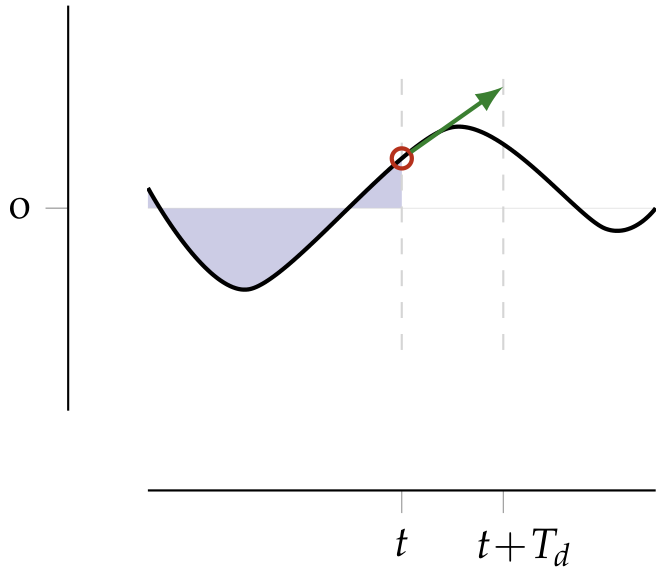
\includegraphics[width=6cm,height=\textheight]{images/pid_regler/pid_graph.png}

}

\end{figure}

\begin{center}
  \begin{tikzpicture}

    \node[box, minimum height=0.8cm, minimum width=1.5cm, inner sep=5pt] (procP) at (0,1) {$k_p$};
    \node[box, minimum height=0.8cm, minimum width=1.5cm, inner sep=5pt] (procI) at (0,0) {$k_i\int dt$};
    \node[box, minimum height=0.8cm, minimum width=1.5cm, inner sep=5pt] (procD) at (0,-1) {$k_d \frac{d}{dt}$};

    \node[dot](startDot) at (-1.5,0) {};
    \node[sum](endSum) at (1.5,0) {+};
\node(start) at (-2.5,0) {$e$};
\node(end) at (2.5,0) {$u$};
\draw  (start) edge (startDot);
\draw[->]  (startDot) |- (procP);
\draw[->]  (startDot) -- (procI);
\draw[->]  (startDot) |- (procD);
\draw[->]  (procD) -| (endSum);
\draw[->]  (procI) -- (endSum);
\draw[->]  (procP) -| (endSum);
\draw[->] (endSum) edge (end);
\end{tikzpicture}
\end{center}

\[
\begin{split}
C(s) & =k_p\left(1+\frac1{T_i\cdot s}+T_d\cdot s\right)=k_p\cdot\frac{(1+sT_1)(1+sT_2)}{T_i\cdot s} \\
&= \underbrace{k_p\cdot e}_{\textcolor{BrickRed}{\text{P}}}+\underbrace{\frac{k_p}{T_i}\int_0^te(\tau)d\tau}_{\textcolor{NavyBlue}{\text{I}}}+\underbrace{k_p\cdot T_d\frac{de}{dt}}_{{\textcolor{OliveGreen}{\text{D}}}}
\end{split}
\]

\begin{conditions}
  k_p & Reglerverstärkung \\
  T_i=\sfrac{k_p}{k_i} & Nachstellzeit \\
  T_d=\sfrac{k_d}{k_o} & Vorhaltzeit
\end{conditions}

\begin{tcolorbox}[enhanced jigsaw, opacitybacktitle=0.6, coltitle=black, arc=.35mm, title=\textcolor{quarto-callout-important-color}{\faExclamation}\hspace{0.5em}{Wichtig}, opacityback=0, colframe=quarto-callout-important-color-frame, left=2mm, bottomtitle=1mm, toptitle=1mm, toprule=.15mm, breakable, leftrule=.75mm, colback=white, titlerule=0mm, bottomrule=.15mm, rightrule=.15mm, colbacktitle=quarto-callout-important-color!10!white]

Diese Beschreibung ist nur eine \ul{idealisierte} Repräsentation, welche
für das Verständnis des System hilfreich ist. Im \ul{praktischen}
Einsatz sind Modifikationen notwendig.

\end{tcolorbox}

\hypertarget{k_p}{%
\subsubsection{\texorpdfstring{\textcolor{BrickRed}{Proportional}
\(k_p\)}{ k\_p}}\label{k_p}}

P-Anteil verstärkt den Regelfehler \(e\) um die
\emph{Proportionalverstärkung} \(k_p\).

\[
C(s) = k_p \qquad u = k_p\cdot e
\]

\begin{tcolorbox}[enhanced jigsaw, opacitybacktitle=0.6, coltitle=black, arc=.35mm, title=\textcolor{quarto-callout-important-color}{\faExclamation}\hspace{0.5em}{Proportionalband}, opacityback=0, colframe=quarto-callout-important-color-frame, left=2mm, bottomtitle=1mm, toptitle=1mm, toprule=.15mm, breakable, leftrule=.75mm, colback=white, titlerule=0mm, bottomrule=.15mm, rightrule=.15mm, colbacktitle=quarto-callout-important-color!10!white]

\[
u = \left\{
\begin{array}{cl}
u_{max} & \text{falls } e \geq e_{max} \\
k_p\cdot e & \text{falls } e_{min} < e < e_{max} \\
u_{min} & \text{falls } e \geq e_{min}
\end{array}
\right.
\]

mit

\[
e_{min}=\frac{u_{min}}{k_p} \qquad e_{max}=\frac{u_{max}}{k_p}
\]

\end{tcolorbox}

\hypertarget{k_it_i}{%
\subsubsection{\texorpdfstring{\textcolor{NavyBlue}{Integral}
\(k_i,T_i\)}{ k\_i,T\_i}}\label{k_it_i}}

Mit dem I-Anteil werden \emph{vergangene} Fehler mitberechnet
\(\rightarrow\) stationäre Fehler des P-Anteils wird korrigiert.

Die Stellgrösse wird dadurch solange geregelt, bis der Regelfehler
\(e=0\) wird.

\hypertarget{k_dt_d}{%
\subsubsection{\texorpdfstring{\textcolor{OliveGreen}{Differential}
\(k_d,T_d\)}{ k\_d,T\_d}}\label{k_dt_d}}

Der D-Anteil reagiert auf \emph{zukünftige} Fehler, indem die Steigung
mit einem Verstärkungsfaktor \(k_d\) verstärkt wird.

\hypertarget{auslegung-anhand}{%
\subsection{Auslegung anhand\ldots{}}\label{auslegung-anhand}}

\hypertarget{modelle-geringer-ordnung}{%
\subsubsection{\ldots Modelle geringer
Ordnung}\label{modelle-geringer-ordnung}}

\hypertarget{approximation-0-er-ordnung}{%
\paragraph{Approximation 0-er
Ordnung}\label{approximation-0-er-ordnung}}

\begin{figure}[H]

{\centering 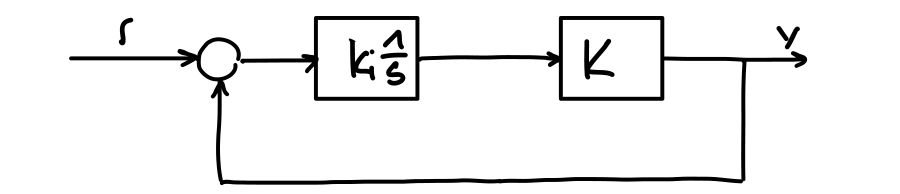
\includegraphics{images/paste-31.png}

}

\end{figure}

Für einen statischen Prozess \(K=P(0)\) und einen I-Regler wird
\(L=PC=K\cdot\frac{k_i}{s}\):

\[
G_{yr}=\frac{K\cdot k_i}{s+K\cdot k_i}=\frac1{1+s\cdot T_{cl}}
\]

\[
k_i = \frac{1}{T_{cl}\cdot K}=\frac1{T_{cl}\cdot P(0)}
\]

\begin{tcolorbox}[enhanced jigsaw, opacitybacktitle=0.6, coltitle=black, arc=.35mm, title=\textcolor{quarto-callout-caution-color}{\faFire}\hspace{0.5em}{mittlere Verzögerungszeit}, opacityback=0, colframe=quarto-callout-caution-color-frame, left=2mm, bottomtitle=1mm, toptitle=1mm, toprule=.15mm, breakable, leftrule=.75mm, colback=white, titlerule=0mm, bottomrule=.15mm, rightrule=.15mm, colbacktitle=quarto-callout-caution-color!10!white]

Die Auslegung bedingt, dass der Prozess gut durch eine Konstante
beschrieben werden kann. Ein vernünftiges Kriterium dafür ist die
Bedingung:

\[
T_{cl}>T_{ar}\qquad T_{ar}=-\frac{P'(0)}{P(0)}
\]

\begin{conditions}
  T_{ar} & mittlere Verzögerungszeit \\
  T_{cl} & Zeitkonstante des geschlossenen Kreises
\end{conditions}

\(T_{ar}\) beschreibt die Zeit, bis die Sprungantwort des Systems sich
gesetzt hat.

\end{tcolorbox}

\hypertarget{approximation-1-ter-ordnung}{%
\paragraph{Approximation 1-ter
Ordnung}\label{approximation-1-ter-ordnung}}

Näherung erster Ordnung kann folgendes Modell gewählt werden.

\[
P\approx P(0)+P'(0)s\approx \frac{P(0)}{1+sT_{ar}}
\]

\hypertarget{bodediagramm}{%
\subsubsection{\ldots Bodediagramm}\label{bodediagramm}}

Diese Auslegung wird mit dem \textbf{offenen} Regelkreis gemacht.

\[
C(s) = k_i \frac{(1+s\ T_1)(1+s\ T_2)}{s} = k_p \frac{(1+s\ T_i)(1+s\ T_d)}{s\cdot T_i}
\]

\ul{Zielgrössen}: Durchtrittsfrequenz \(\omega_{gc}\), die Phasenreserve
\(\varphi_m\) und allenfalls Amplitudenreserve \(g_m\).

\begin{tcolorbox}[enhanced jigsaw, opacitybacktitle=0.6, coltitle=black, arc=.35mm, title=\textcolor{quarto-callout-tip-color}{\faLightbulb}\hspace{0.5em}{Vorgehen}, opacityback=0, colframe=quarto-callout-tip-color-frame, left=2mm, bottomtitle=1mm, toptitle=1mm, toprule=.15mm, breakable, leftrule=.75mm, colback=white, titlerule=0mm, bottomrule=.15mm, rightrule=.15mm, colbacktitle=quarto-callout-tip-color!10!white]

Prozess: \(P(s)=\frac{10}{(1+s)^2}\) mit Ziel
\(\omega_{gc}\geq 10 \frac{rad}{s}\), \(\varphi_m\geq 50°\).

\begin{enumerate}
\def\labelenumi{\arabic{enumi}.}
\tightlist
\item
  P-Regler für Erreichung von \(\omega_{gc}\). Mit
  \(\lvert k_p\cdot P(j\omega_{gc})\rvert = 1\) (Nyquist-Kriterium)
  folgt:
\end{enumerate}

\[
k_p = \frac{1}{\left\lvert\frac{10}{1+10j}\right\rvert} = \frac{(\sqrt{1^2+10^2})^2}{10}=10.1
\]

\[
\textcolor{BrickRed}{C(s)}=k_p=10.1
\]

\begin{enumerate}
\def\labelenumi{\arabic{enumi}.}
\setcounter{enumi}{1}
\tightlist
\item
  PI-Regler für Reduktion der zusätzlichen Phasensenkung im Bereich von
  \(\omega_{gc}\)
\end{enumerate}

\[
\textcolor{NavyBlue}{C(s)} = k_i\cdot\frac{(1+s\cdot T_1)}{s} = \frac{10\cdot(1+s)}{s}
\]

\begin{enumerate}
\def\labelenumi{\arabic{enumi}.}
\tightlist
\item
  PID-Regler für genügend Phasenabhebung im Bereich von \(\omega_{gc}\)
\end{enumerate}

\[
\begin{split}
\textcolor{OliveGreen}{C(s)} &= k_i\cdot\frac{(1+s\cdot T_1)(1+s\cdot T_2)}{s} \\ &= 10\cdot\frac{(1+s)(1+0.1s)}{s}
\end{split}
\]

\begin{enumerate}
\def\labelenumi{\arabic{enumi}.}
\setcounter{enumi}{3}
\tightlist
\item
  Kontrolle von resultiernden Durchtrittsfrequenz \(\omega_{gc}'\) und
  damit ergebenden Phasenreserve \(\varphi_m\).
\end{enumerate}

\begin{figure}[H]

{\centering 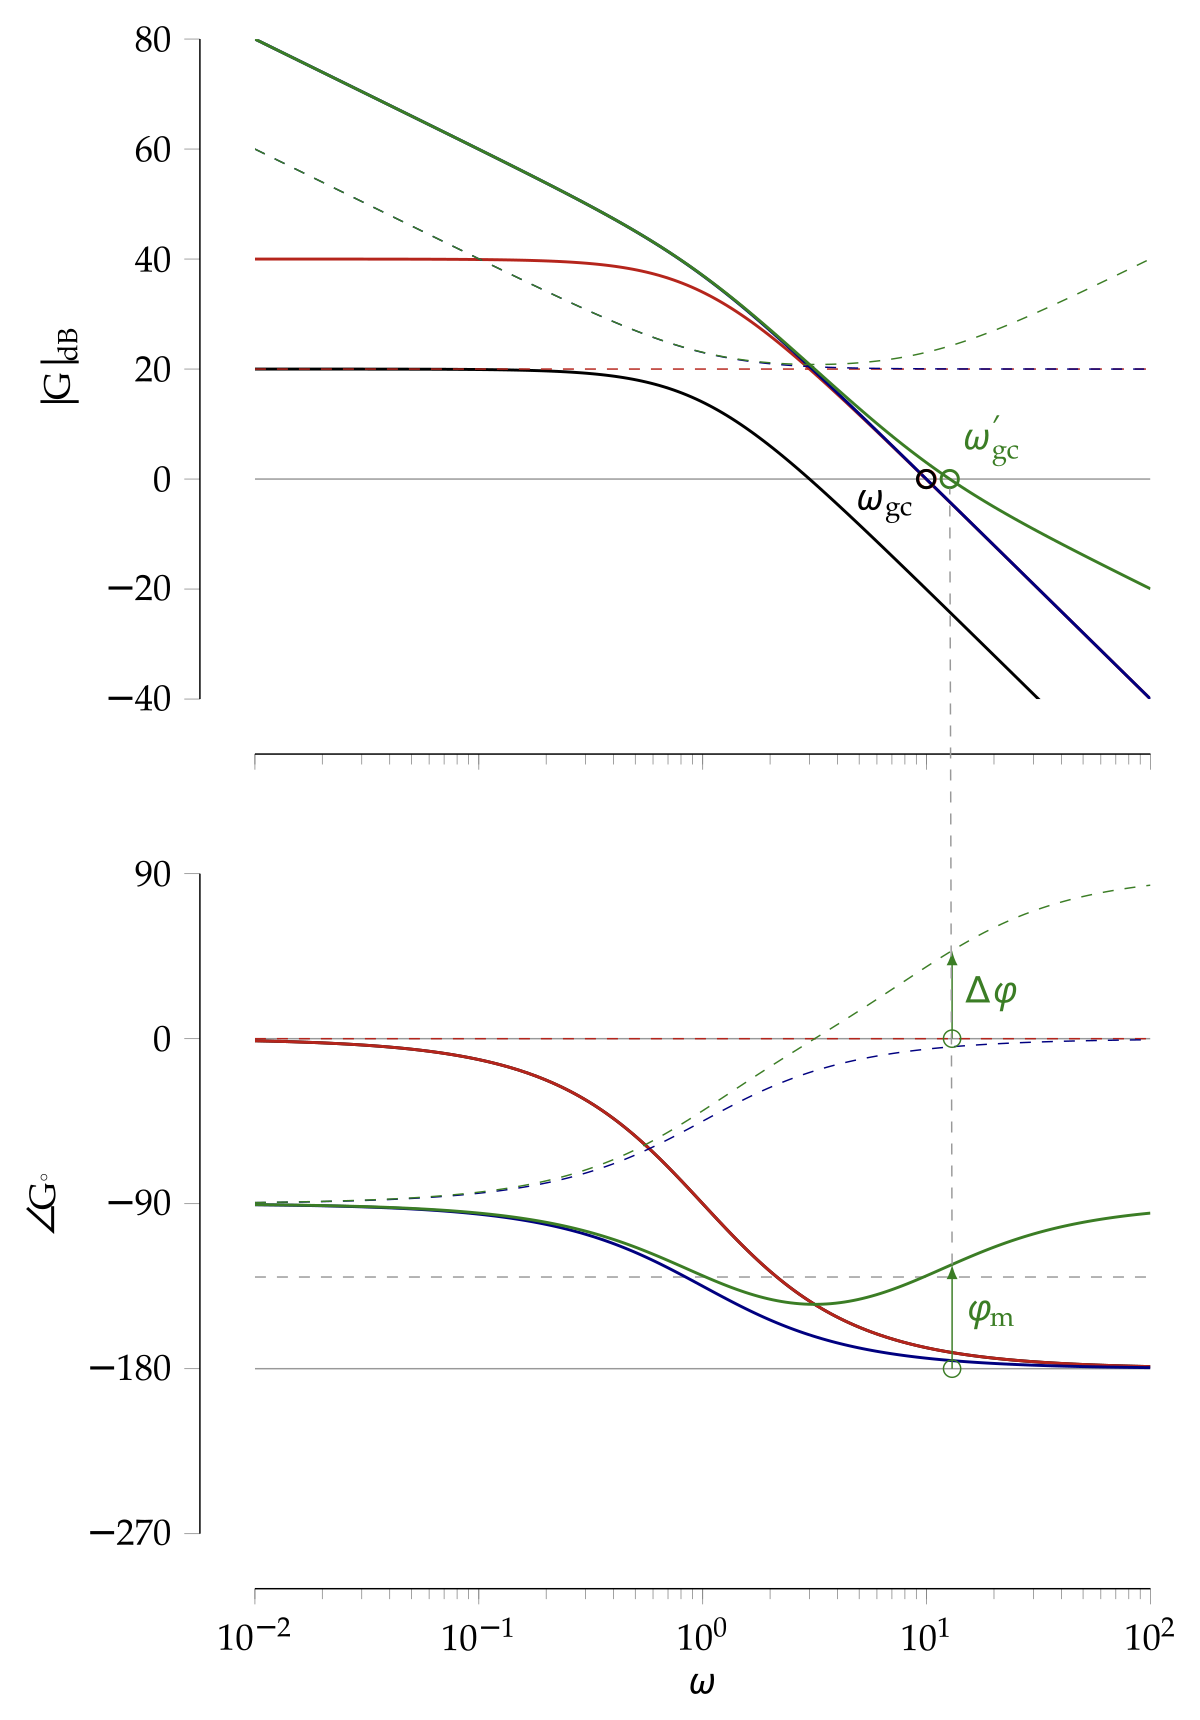
\includegraphics{images/pid_regler/auslegung_bodediagramm.png}

}

\end{figure}

\end{tcolorbox}

\hypertarget{einstellregeln-im-zeitbereich}{%
\subsubsection{\ldots Einstellregeln im
Zeitbereich}\label{einstellregeln-im-zeitbereich}}

\begin{figure}[H]

{\centering 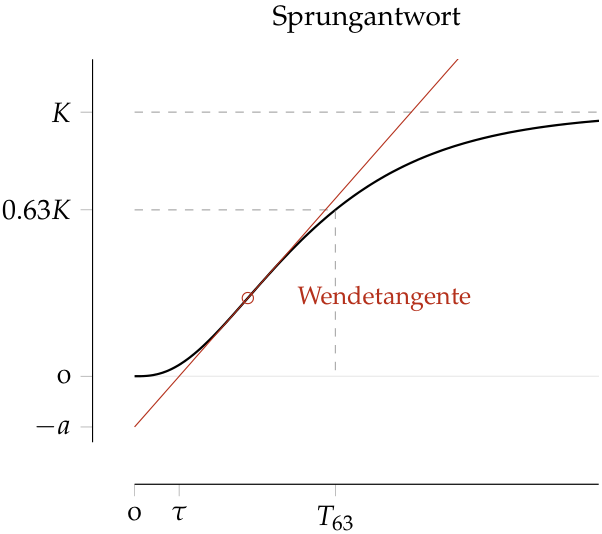
\includegraphics[width=6cm,height=\textheight]{images/paste-25.png}

}

\end{figure}

\begin{longtable}[]{@{}cccc@{}}
\toprule\noalign{}
Typ & \(k_p\) & \(T_i\) & \(T_d\) \\
\midrule\noalign{}
\endhead
\bottomrule\noalign{}
\endlastfoot
P & \(\sfrac{1}{a}\) & - & - \\
PI & \(\sfrac{0.9}{a}\) & \(3\cdot\tau\) & - \\
PID & \(\sfrac{1.2}{a}\) & \(2\cdot\tau\) & \(0.5\cdot\tau\) \\
\end{longtable}

\hypertarget{einstellregeln-im-frequenzbereich}{%
\subsubsection{\ldots Einstellregeln im
Frequenzbereich}\label{einstellregeln-im-frequenzbereich}}

Verstärkung \(k\) erhöhen, bis sich eine anhaltende Schwingung
einstellt. Regelparameter anhand kritischer Verstärkung \(k_c\) \&
Periodendauer \(T_c\) ermitteln.

\begin{figure}[H]

{\centering 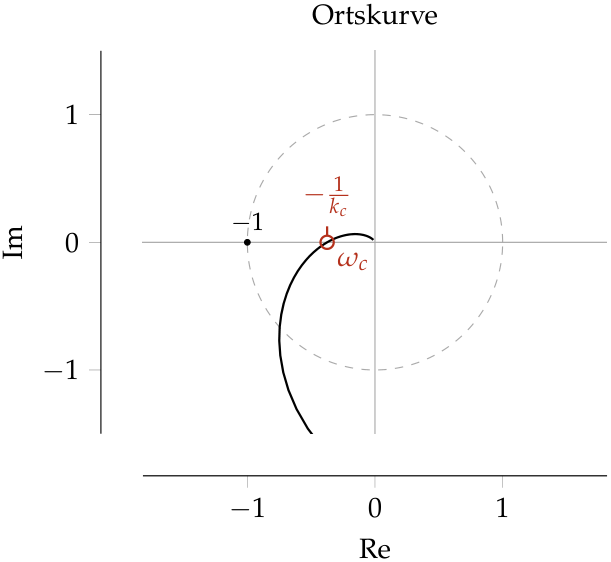
\includegraphics[width=6cm,height=\textheight]{images/paste-26.png}

}

\end{figure}

\begin{longtable}[]{@{}cccc@{}}
\toprule\noalign{}
Typ & \(k_p\) & \(T_i\) & \(T_d\) \\
\midrule\noalign{}
\endhead
\bottomrule\noalign{}
\endlastfoot
P & \(0.5\cdot k_c\) & \(-\) & \(-\) \\
PI & \(0.4\cdot k_c\) & \(0.8\cdot T_c\) & \(-\) \\
PID & \(0.6\cdot k_c\) & \(0.5\cdot T_c\) & \(0.125\cdot T_c\) \\
\end{longtable}

\hypertarget{stellgruxf6ssen-suxe4ttigung}{%
\subsection{Stellgrössen-Sättigung}\label{stellgruxf6ssen-suxe4ttigung}}

\begin{tcolorbox}[enhanced jigsaw, opacitybacktitle=0.6, coltitle=black, arc=.35mm, title=\textcolor{quarto-callout-warning-color}{\faExclamationTriangle}\hspace{0.5em}{Sättigungseffekt}, opacityback=0, colframe=quarto-callout-warning-color-frame, left=2mm, bottomtitle=1mm, toptitle=1mm, toprule=.15mm, breakable, leftrule=.75mm, colback=white, titlerule=0mm, bottomrule=.15mm, rightrule=.15mm, colbacktitle=quarto-callout-warning-color!10!white]

Arbeitet der Regelkreis in der Sättigung, so ist dieser faktisch
unterbrochen -- \emph{das System arbeitet als offener Kreis}, solange
der Aktor im gesättigtem Zustand ist.

\end{tcolorbox}

\hypertarget{windup}{%
\subsubsection{Windup}\label{windup}}

Bei Sättigung baut Fehler den I-Anteil auf. Muss nach Erholung abgebaut
werden.

\begin{figure}[H]

{\centering 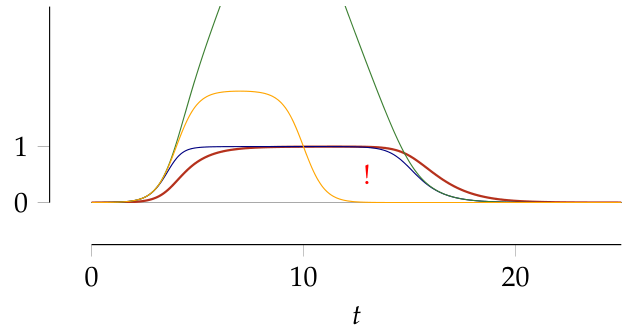
\includegraphics[width=6.5cm,height=3.4cm]{images/paste-27.png}

}

\end{figure}

\begin{figure}[H]

{\centering 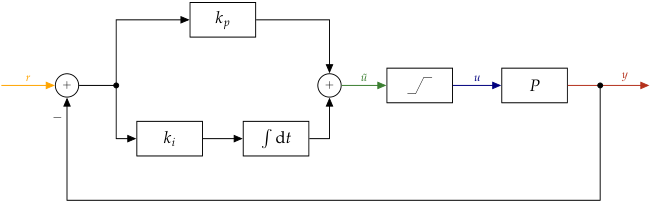
\includegraphics[width=8cm,height=2.6cm]{images/paste-28.png}

}

\end{figure}

\hypertarget{anti-windup}{%
\subsubsection{Anti-Windup}\label{anti-windup}}

Exzessiver Anteil wird mit einem invertierten Vorzeichen an den
Integrator zurückgeführt und somit der Windup klein gehalten
\(\rightarrow\) kürzere \emph{Erholzeit}~nach Stellgrössensättigung

\begin{figure}[H]

{\centering 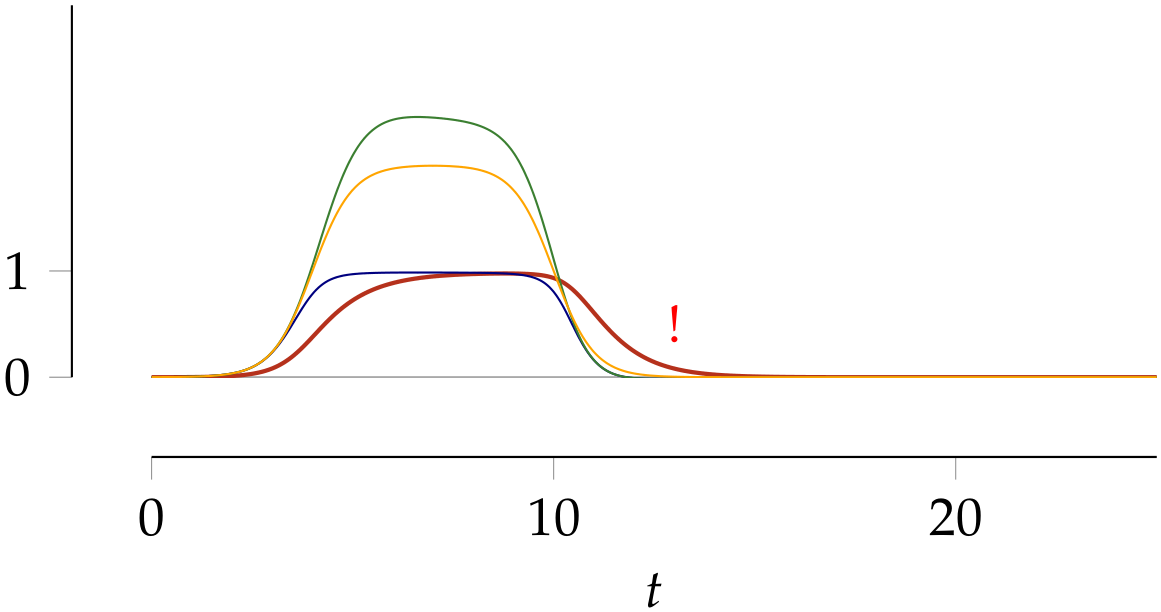
\includegraphics[width=6.5cm,height=\textheight]{images/paste-30.png}

}

\end{figure}

\begin{figure}[H]

{\centering 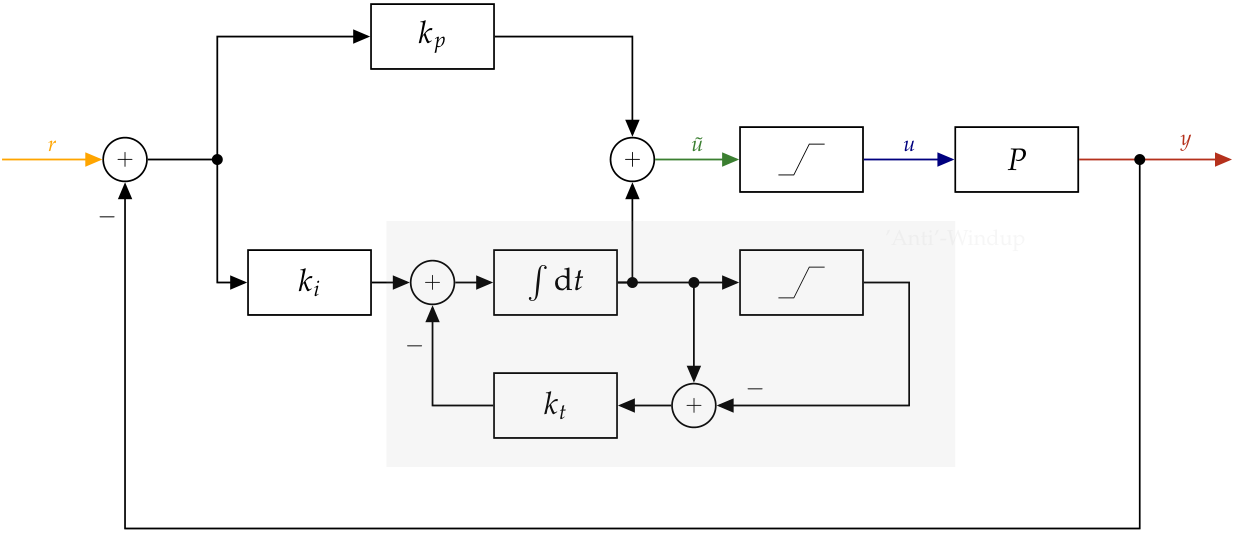
\includegraphics[width=8cm,height=3.5cm]{images/paste-29.png}

}

\end{figure}

\[
k_t \approx 10 k_i
\]

\hypertarget{loop-shaping}{%
\section{Loop Shaping}\label{loop-shaping}}

\begin{tcolorbox}[enhanced jigsaw, opacitybacktitle=0.6, coltitle=black, arc=.35mm, title=\textcolor{quarto-callout-important-color}{\faExclamation}\hspace{0.5em}{Verlauf von \(\lvert L\rvert\)}, opacityback=0, colframe=quarto-callout-important-color-frame, left=2mm, bottomtitle=1mm, toptitle=1mm, toprule=.15mm, breakable, leftrule=.75mm, colback=white, titlerule=0mm, bottomrule=.15mm, rightrule=.15mm, colbacktitle=quarto-callout-important-color!10!white]

\[
\begin{array}{ll}
\omega < \omega_{gc} & \text{möglichst gross} \\
\omega \approx \omega_{gc} & \text{möglichst flach} \\
\omega > \omega_{gc} & \text{möglichst klein}
\end{array}
\]

\end{tcolorbox}

\begin{figure}[H]

{\centering 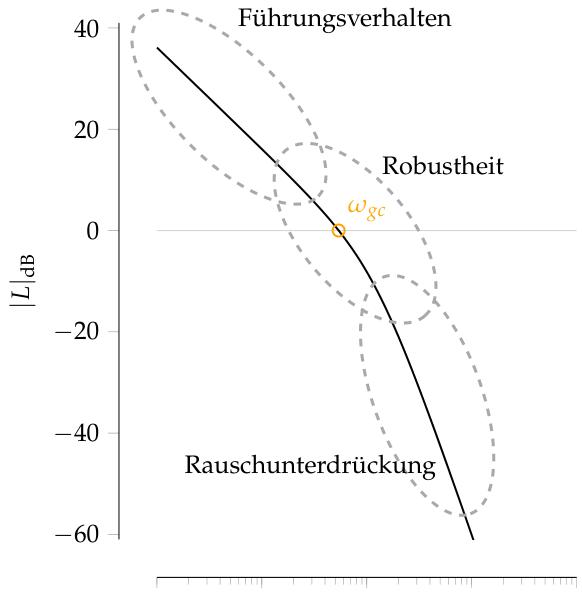
\includegraphics[width=6cm,height=\textheight]{images/paste-38.png}

}

\end{figure}

\begin{figure}[H]

{\centering 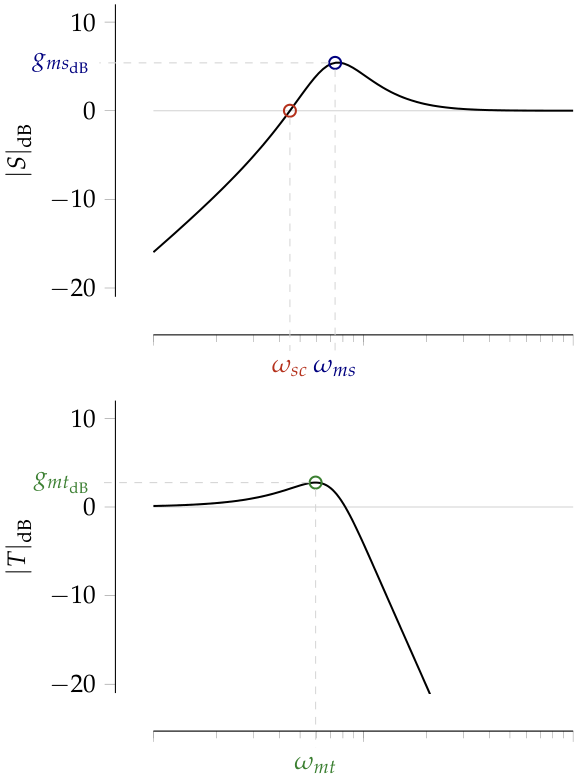
\includegraphics[width=6cm,height=\textheight]{images/paste-39.png}

}

\end{figure}

\hypertarget{lag-lead-kompensatoren}{%
\subsection{Lag \& Lead Kompensatoren}\label{lag-lead-kompensatoren}}

\[
C(s)=k\cdot \prod_i \left(\frac{s+a_i}{s+b_i}\right)
\]

Mit \(a_i > 0, b_i > 0, k > 0\)

\begin{tcolorbox}[enhanced jigsaw, opacitybacktitle=0.6, coltitle=black, arc=.35mm, title=\textcolor{quarto-callout-note-color}{\faInfo}\hspace{0.5em}{PI-Regler \& D-Anteil}, opacityback=0, colframe=quarto-callout-note-color-frame, left=2mm, bottomtitle=1mm, toptitle=1mm, toprule=.15mm, breakable, leftrule=.75mm, colback=white, titlerule=0mm, bottomrule=.15mm, rightrule=.15mm, colbacktitle=quarto-callout-note-color!10!white]

PI Regler \(\rightarrow\ b = 0\)

D-Anteil mit Beschränkung \(\rightarrow\ a = 0\)

\end{tcolorbox}

\hypertarget{lead-a-b}{%
\subsubsection{\texorpdfstring{Lead
(\(a < b\))}{Lead (a \textless{} b)}}\label{lead-a-b}}

Verstärkung bei hohen Frequenzen + Phasenanhebung (\(\max 90\degree\)
pro Ordnung)

\begin{figure}[H]

{\centering 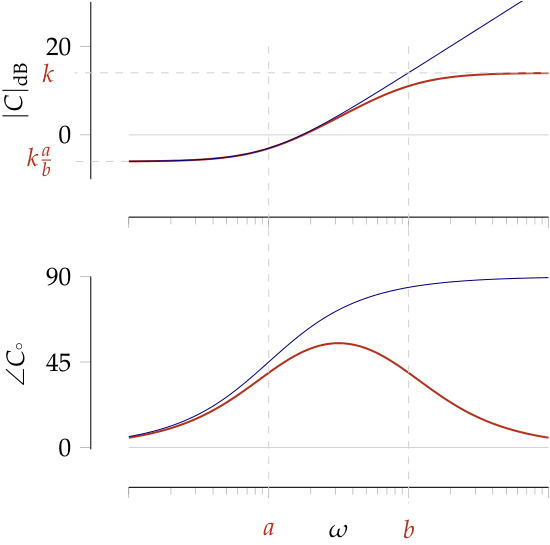
\includegraphics[width=7cm,height=\textheight]{images/paste-40.png}

}

\end{figure}

\hypertarget{lag-a-b}{%
\subsubsection{\texorpdfstring{Lag
(\(a > b\))}{Lag (a \textgreater{} b)}}\label{lag-a-b}}

Verstärkung bei tiefen Frequenzen + Phasensenkung (\(\max -90\degree\)
pro Ordnung)

\begin{figure}[H]

{\centering 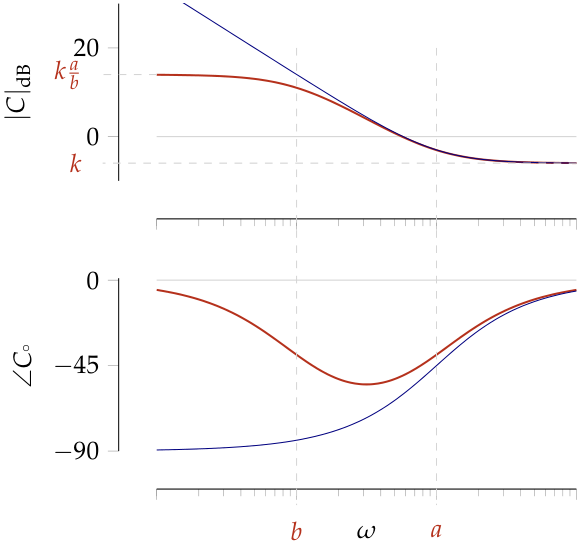
\includegraphics[width=7cm,height=\textheight]{images/paste-41.png}

}

\end{figure}

\hypertarget{grenzen-des-loop-shapings}{%
\subsection{Grenzen des Loop-Shapings}\label{grenzen-des-loop-shapings}}

Der Beeinflussing des Systemverhalten durch Regelung sind bestimmte
Grenzen gesetzt. Verhalten kann nicht uniform verbessert werden.

\begin{tcolorbox}[enhanced jigsaw, opacitybacktitle=0.6, coltitle=black, arc=.35mm, title=\textcolor{quarto-callout-note-color}{\faInfo}\hspace{0.5em}{Bode's Integral}, opacityback=0, colframe=quarto-callout-note-color-frame, left=2mm, bottomtitle=1mm, toptitle=1mm, toprule=.15mm, breakable, leftrule=.75mm, colback=white, titlerule=0mm, bottomrule=.15mm, rightrule=.15mm, colbacktitle=quarto-callout-note-color!10!white]

Ist der geschlossene Regelkreis mit \(L\) stabil und geht \(sL(s)\) für
\(s\rightarrow\infty\) gegen null, dann ist

\[
\int_0^\infty \log\lvert S(j\omega)\rvert\ d\omega = \pi \sum p_k
\]

wobei \(p_k\) die Pole in der \ul{rechten} Halbebene sind. Ist \(L\) an
sich stabil, so gilt

\[
\int_0^\infty\log\lvert S(j\omega)\rvert\ d\omega = 0
\]

\end{tcolorbox}

\textbf{Alle Verbesserungen werden mit Verschlechterungen
komplementiert.}

\begin{figure}[H]

{\centering 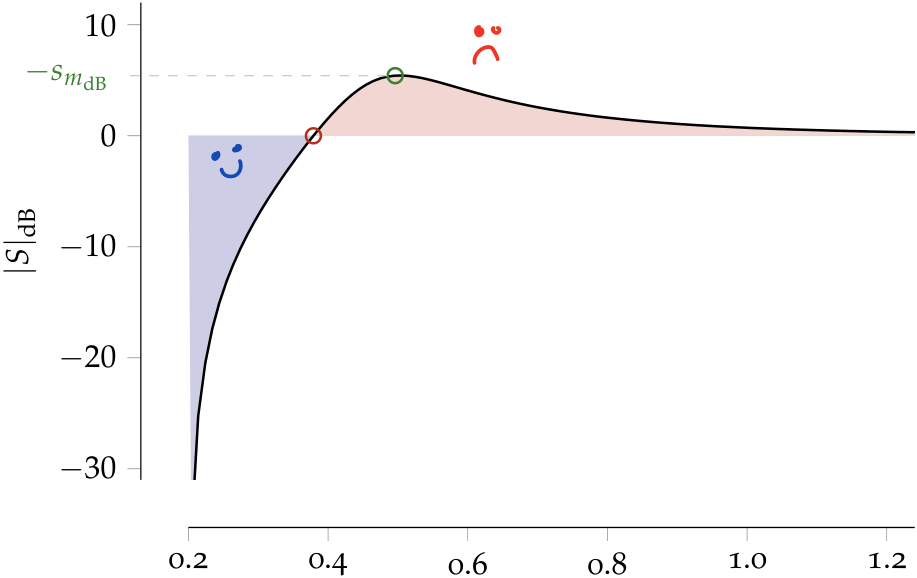
\includegraphics{images/paste-42.png}

}

\end{figure}

\hypertarget{diskretisierung}{%
\section{Diskretisierung}\label{diskretisierung}}

\hypertarget{pid-regler-1}{%
\subsection{PID-Regler}\label{pid-regler-1}}

\hypertarget{auslegung}{%
\subsection{Auslegung}\label{auslegung}}

Digitalrechner arbeiten zeitdiskret \(\leftrightarrow\) Prozesse sind
von zeitkontinuierlicher Natur

\begin{tcolorbox}[enhanced jigsaw, opacitybacktitle=0.6, coltitle=black, arc=.35mm, title=\textcolor{quarto-callout-note-color}{\faInfo}\hspace{0.5em}{Perspektiven für Entwurf zeitdiskrete Regler}, opacityback=0, colframe=quarto-callout-note-color-frame, left=2mm, bottomtitle=1mm, toptitle=1mm, toprule=.15mm, breakable, leftrule=.75mm, colback=white, titlerule=0mm, bottomrule=.15mm, rightrule=.15mm, colbacktitle=quarto-callout-note-color!10!white]

\begin{enumerate}
\def\labelenumi{\arabic{enumi}.}
\tightlist
\item
  \emph{Prozess}:
\item
  \emph{Regler}:
\end{enumerate}

\end{tcolorbox}

\hypertarget{matlab}{%
\section{MATLAB}\label{matlab}}

\hypertarget{vektoren}{%
\subsection{Vektoren}\label{vektoren}}

Vektoren werden mit \texttt{{[}…{]}} deklariert. Elemente werden
Spaltenweise mit einem Leerschlag
\texttt{\textquotesingle{}\ \textquotesingle{}} oder Komma \texttt{,}
eingeteilt und mit einem Semikolon \texttt{;} Reihenweise geteilt.

\begin{Shaded}
\begin{Highlighting}[]
\VariableTok{data} \OperatorTok{=}\NormalTok{ [}\FloatTok{1}\OperatorTok{,}\FloatTok{2}\OperatorTok{,}\FloatTok{3}\OperatorTok{;}\FloatTok{4}\OperatorTok{,}\FloatTok{5}\OperatorTok{,}\FloatTok{6}\OperatorTok{;}\FloatTok{7}\OperatorTok{,}\FloatTok{8}\OperatorTok{,}\FloatTok{9}\NormalTok{]}\OperatorTok{;} \CommentTok{\% same as [1 2 3;4 5 6;7 8 9];}
\end{Highlighting}
\end{Shaded}

\begin{tcolorbox}[enhanced jigsaw, opacitybacktitle=0.6, coltitle=black, arc=.35mm, title=\textcolor{quarto-callout-note-color}{\faInfo}\hspace{0.5em}{Grösse \texttt{size}}, opacityback=0, colframe=quarto-callout-note-color-frame, left=2mm, bottomtitle=1mm, toptitle=1mm, toprule=.15mm, breakable, leftrule=.75mm, colback=white, titlerule=0mm, bottomrule=.15mm, rightrule=.15mm, colbacktitle=quarto-callout-note-color!10!white]

Mit \texttt{size} kann die Grösse einer Variable ermittelt werden.
\texttt{size} gibt als Resultat ein 1x2 Vektor zurück
(\(\begin{bmatrix}\text{Rows} & \text{Columns}\end{bmatrix}\))

\begin{Shaded}
\begin{Highlighting}[]
\OperatorTok{\textgreater{}\textgreater{}} \VariableTok{a} \OperatorTok{=} \FloatTok{1}
\OperatorTok{\textgreater{}\textgreater{}} \VariableTok{size}\NormalTok{(}\VariableTok{a}\NormalTok{)}
     \FloatTok{1}     \FloatTok{1}  \CommentTok{\% rows, columns}
\end{Highlighting}
\end{Shaded}

\end{tcolorbox}

\begin{Shaded}
\begin{Highlighting}[]
\VariableTok{a} \OperatorTok{=} \FloatTok{1}
\end{Highlighting}
\end{Shaded}

\[
\begin{bmatrix}
1
\end{bmatrix}\qquad \text{oder einfach}\qquad 1 
\]

Die \texttt{size}-Funktion gibt auch bei einzelnen Werte eine Grösse
aus, nämlich \(\begin{bmatrix}1 & 1\end{bmatrix}\)

\begin{Shaded}
\begin{Highlighting}[]
\VariableTok{b} \OperatorTok{=}\NormalTok{ [}\FloatTok{1} \FloatTok{2} \FloatTok{3}\NormalTok{] }\CommentTok{\% Linienvektor}
\end{Highlighting}
\end{Shaded}

\[
\begin{bmatrix}
1 & 2 & 3
\end{bmatrix}
\]

\begin{Shaded}
\begin{Highlighting}[]
\VariableTok{c} \OperatorTok{=}\NormalTok{ [}\FloatTok{2}\OperatorTok{;}\FloatTok{3}\OperatorTok{;}\FloatTok{4}\NormalTok{] }\CommentTok{\% Spaltenvektor}
\end{Highlighting}
\end{Shaded}

\[
\begin{bmatrix}
2 \\ 3 \\ 4
\end{bmatrix}
\]

\begin{tcolorbox}[enhanced jigsaw, opacitybacktitle=0.6, coltitle=black, arc=.35mm, title=\textcolor{quarto-callout-tip-color}{\faLightbulb}\hspace{0.5em}{Slicing}, opacityback=0, colframe=quarto-callout-tip-color-frame, left=2mm, bottomtitle=1mm, toptitle=1mm, toprule=.15mm, breakable, leftrule=.75mm, colback=white, titlerule=0mm, bottomrule=.15mm, rightrule=.15mm, colbacktitle=quarto-callout-tip-color!10!white]

Mit \emph{Slicing} kann ein Teil einer Matrix \textbf{kopiert} werden
und einer anderen Variable zugewiesen werden.

\begin{Shaded}
\begin{Highlighting}[]
\OperatorTok{\textless{}}\VariableTok{matrix}\OperatorTok{\textgreater{}}\NormalTok{(}\OperatorTok{\textless{}}\VariableTok{rowStart}\OperatorTok{\textgreater{}:\textless{}}\VariableTok{rowEnd}\OperatorTok{\textgreater{},\textless{}}\VariableTok{colStart}\OperatorTok{\textgreater{}:\textless{}}\VariableTok{colEnd}\OperatorTok{\textgreater{}}\NormalTok{)}
\end{Highlighting}
\end{Shaded}

\end{tcolorbox}

\hypertarget{plotting}{%
\subsection{Plotting}\label{plotting}}

\begin{tcolorbox}[enhanced jigsaw, opacitybacktitle=0.6, coltitle=black, arc=.35mm, title=\textcolor{quarto-callout-note-color}{\faInfo}\hspace{0.5em}{Figure-Separierung}, opacityback=0, colframe=quarto-callout-note-color-frame, left=2mm, bottomtitle=1mm, toptitle=1mm, toprule=.15mm, breakable, leftrule=.75mm, colback=white, titlerule=0mm, bottomrule=.15mm, rightrule=.15mm, colbacktitle=quarto-callout-note-color!10!white]

Mit \texttt{figure(n)} können mehrere Plot-Befehle in eigene Figuren
geladen werden.

\end{tcolorbox}

\hypertarget{xy-graph}{%
\subsubsection{XY-Graph}\label{xy-graph}}

\begin{Shaded}
\begin{Highlighting}[]
\VariableTok{figure}\NormalTok{(}\FloatTok{1}\NormalTok{)}\OperatorTok{;}
\VariableTok{t} \OperatorTok{=} \FloatTok{0}\OperatorTok{:}\FloatTok{0.5}\OperatorTok{:}\FloatTok{10}\OperatorTok{;}
\VariableTok{y} \OperatorTok{=} \VariableTok{sin}\NormalTok{(}\VariableTok{t}\NormalTok{)}\OperatorTok{;}

\VariableTok{plot}\NormalTok{(}\VariableTok{t}\OperatorTok{,}\VariableTok{y}\NormalTok{)}\OperatorTok{;}
\VariableTok{xlim}\NormalTok{([}\OperatorTok{{-}}\FloatTok{0.5} \FloatTok{10.5}\NormalTok{])}\OperatorTok{;}
\VariableTok{ylim}\NormalTok{([}\OperatorTok{{-}}\FloatTok{1.1} \FloatTok{1.1}\NormalTok{])}\OperatorTok{;}
\end{Highlighting}
\end{Shaded}

\begin{figure}[H]

{\centering \includegraphics{images/plot_simple.png}

}

\end{figure}

\hypertarget{xyy-graph}{%
\subsubsection{XYY-Graph}\label{xyy-graph}}

Mit \texttt{yyaxis} kann die Y-Achse beim selben Plot mit \texttt{left}
\& \texttt{right} gewechselt werden.

\begin{Shaded}
\begin{Highlighting}[]
\VariableTok{figure}\NormalTok{(}\FloatTok{1}\NormalTok{)}\OperatorTok{;}
\VariableTok{t} \OperatorTok{=} \FloatTok{0}\OperatorTok{:}\FloatTok{0.5}\OperatorTok{:}\FloatTok{10}\OperatorTok{;}

\VariableTok{yyaxis} \VariableTok{left}\OperatorTok{;}
\VariableTok{plot}\NormalTok{(}\VariableTok{t}\OperatorTok{,} \VariableTok{sin}\NormalTok{(}\VariableTok{t}\NormalTok{))}\OperatorTok{;}
\VariableTok{xlim}\NormalTok{([}\OperatorTok{{-}}\FloatTok{0.5} \FloatTok{10.5}\NormalTok{])}\OperatorTok{;}
\VariableTok{ylim}\NormalTok{([}\OperatorTok{{-}}\FloatTok{1.1} \FloatTok{1.1}\NormalTok{])}\OperatorTok{;}

\VariableTok{yyaxis} \VariableTok{right}\OperatorTok{;}
\VariableTok{plot}\NormalTok{(}\VariableTok{t}\OperatorTok{,} \FloatTok{20}\OperatorTok{*}\VariableTok{cos}\NormalTok{(}\VariableTok{t}\NormalTok{))}\OperatorTok{;}
\VariableTok{xlim}\NormalTok{([}\OperatorTok{{-}}\FloatTok{0.5} \FloatTok{10.5}\NormalTok{])}\OperatorTok{;}
\VariableTok{ylim}\NormalTok{([}\OperatorTok{{-}}\FloatTok{20.5} \FloatTok{20.5}\NormalTok{])}\OperatorTok{;}
\end{Highlighting}
\end{Shaded}

\begin{figure}[H]

{\centering \includegraphics{images/plotyy.png}

}

\end{figure}

\hypertarget{transferfunktion-tf}{%
\subsection{\texorpdfstring{Transferfunktion
\texttt{tf(…)}}{Transferfunktion tf(\ldots)}}\label{transferfunktion-tf}}

Mit dem Befehl \texttt{tf(...)} kann eine Transferfunktion deklariert
werden mit Zähler- und Nenner-Zeilenvektoren.

\begin{Shaded}
\begin{Highlighting}[]
\VariableTok{sys} \OperatorTok{=} \VariableTok{tf}\NormalTok{(}\VariableTok{numerator}\OperatorTok{,}\VariableTok{denominator}\NormalTok{)}\OperatorTok{;}
\end{Highlighting}
\end{Shaded}

Die Transferfunktion kann in anderen Funktion wiederverwendet werden,
wie zum Beispiel \texttt{step} oder \texttt{bode}. Folgende Beispiele
sind mit der \texttt{sys}-Transferfunktion (folgende Gleichung) gemacht.

\[
G_{\text{sys}}(s) = \frac{4}{s^2+s+10}
\]

\begin{Shaded}
\begin{Highlighting}[]
\VariableTok{sys} \OperatorTok{=} \VariableTok{tf}\NormalTok{(}\FloatTok{4}\OperatorTok{,}\NormalTok{[}\FloatTok{1} \FloatTok{2} \FloatTok{10}\NormalTok{])}\OperatorTok{;}
\end{Highlighting}
\end{Shaded}

\hypertarget{pid-regler-pidstd}{%
\subsubsection{\texorpdfstring{PID-Regler
\texttt{pidstd}}{PID-Regler pidstd}}\label{pid-regler-pidstd}}

\begin{Shaded}
\begin{Highlighting}[]

\end{Highlighting}
\end{Shaded}

\hypertarget{bode-diagramm-bode}{%
\subsubsection{\texorpdfstring{Bode-Diagramm
\texttt{bode}}{Bode-Diagramm bode}}\label{bode-diagramm-bode}}

\begin{Shaded}
\begin{Highlighting}[]
\VariableTok{bode}\NormalTok{(}\VariableTok{sys}\OperatorTok{,}\NormalTok{\{}\FloatTok{0.1}\OperatorTok{,}\FloatTok{100}\NormalTok{\})}\OperatorTok{;} \CommentTok{\% or bode(sys);}
\CommentTok{\% grid on; to enable Grid in Plot}
\end{Highlighting}
\end{Shaded}

\begin{figure}[H]

{\centering \includegraphics{images/matlab_BodePlotResponse.png}

}

\end{figure}

\hypertarget{nyquist-diagramm-nyquist}{%
\subsubsection{\texorpdfstring{Nyquist-Diagramm
\texttt{nyquist}}{Nyquist-Diagramm nyquist}}\label{nyquist-diagramm-nyquist}}

\begin{Shaded}
\begin{Highlighting}[]
\VariableTok{nyquist}\NormalTok{(}\VariableTok{sys}\NormalTok{)}
\end{Highlighting}
\end{Shaded}

\begin{figure}[H]

{\centering \includegraphics{images/matlab_NyquistPlotResponse.png.png}

}

\end{figure}

\hypertarget{sprungantwort-step}{%
\subsubsection{\texorpdfstring{Sprungantwort
\texttt{step}}{Sprungantwort step}}\label{sprungantwort-step}}

Mit \texttt{step(…)} kann eine Transferfunktion mit der Sprungfunktion
\(\sigma\) verwendet werden. Damit

\begin{Shaded}
\begin{Highlighting}[]
\VariableTok{step}\NormalTok{(}\VariableTok{sys}\NormalTok{)}\OperatorTok{;}
\end{Highlighting}
\end{Shaded}

\begin{figure}[H]

{\centering \includegraphics{images/matlab_StepResponsePlot.png}

}

\end{figure}

\hypertarget{impulsantwort-impulse}{%
\subsubsection{\texorpdfstring{Impulsantwort
\texttt{impulse}}{Impulsantwort impulse}}\label{impulsantwort-impulse}}

Mit \texttt{impulse(…)} kann die Impulsantwort der Transferfunktion
ausgegeben werden.

\begin{Shaded}
\begin{Highlighting}[]
\VariableTok{impulse}\NormalTok{(}\VariableTok{sys}\NormalTok{)}\OperatorTok{;}
\end{Highlighting}
\end{Shaded}

\begin{figure}[H]

{\centering \includegraphics{images/matlab_ImpulseResponsePlot.png}

}

\end{figure}

\hypertarget{pol-nullstellen-diagramm-pzmap}{%
\subsubsection{\texorpdfstring{Pol-Nullstellen-Diagramm
\texttt{pzmap}}{Pol-Nullstellen-Diagramm pzmap}}\label{pol-nullstellen-diagramm-pzmap}}

\begin{Shaded}
\begin{Highlighting}[]
\VariableTok{pzmap}\NormalTok{(}\VariableTok{sys}\NormalTok{)}\OperatorTok{;}
\VariableTok{ylim}\NormalTok{([}\OperatorTok{{-}}\FloatTok{4} \FloatTok{4}\NormalTok{])}\OperatorTok{;} \VariableTok{xlim}\NormalTok{([}\OperatorTok{{-}}\FloatTok{1.2} \FloatTok{0}\NormalTok{])}\OperatorTok{;}
\end{Highlighting}
\end{Shaded}

\begin{figure}[H]

{\centering \includegraphics{images/matlab_PoleZeroMap.png}

}

\end{figure}

\begin{tcolorbox}[enhanced jigsaw, opacitybacktitle=0.6, coltitle=black, arc=.35mm, title=\textcolor{quarto-callout-caution-color}{\faFire}\hspace{0.5em}{MATLAB Zauber}, opacityback=0, colframe=quarto-callout-caution-color-frame, left=2mm, bottomtitle=1mm, toptitle=1mm, toprule=.15mm, breakable, leftrule=.75mm, colback=white, titlerule=0mm, bottomrule=.15mm, rightrule=.15mm, colbacktitle=quarto-callout-caution-color!10!white]

Damit die Pol- und Nullstellen erkennbar sind, muss eventuell mit den
Darstellungsgrenzen gespielt werden.

\end{tcolorbox}

\hypertarget{margin-margintf}{%
\subsection{\texorpdfstring{Margin
\texttt{margin(tf)}}{Margin margin(tf)}}\label{margin-margintf}}

Mit dem Befehl \texttt{margin(tf)} kann das Bode-Diagramm

\begin{Shaded}
\begin{Highlighting}[]
\NormalTok{margin(tf(}\DecValTok{1}\OtherTok{,[}\DecValTok{1} \DecValTok{2} \DecValTok{1} \DecValTok{0}\OtherTok{]}\NormalTok{))}
\end{Highlighting}
\end{Shaded}

\begin{figure}[H]

{\centering \includegraphics{images/PlotGainAndPhaseMarginsOfTransferFunctionExample_01.png}

}

\end{figure}

\hypertarget{zustandsraumdarstellung-ss}{%
\subsection{\texorpdfstring{Zustandsraumdarstellung
\texttt{ss()}}{Zustandsraumdarstellung ss()}}\label{zustandsraumdarstellung-ss}}

Mit \texttt{ss(…)} können vier Matrizen \(A, B,C,D\) zu einer
Zustandsraumdarstellung zusammengeführt werden.

\begin{Shaded}
\begin{Highlighting}[]
\VariableTok{A} \OperatorTok{=}\NormalTok{ [}\FloatTok{0} \FloatTok{1}\OperatorTok{;{-}}\FloatTok{5} \OperatorTok{{-}}\FloatTok{2}\NormalTok{]}\OperatorTok{;}
\VariableTok{B} \OperatorTok{=}\NormalTok{ [}\FloatTok{0}\OperatorTok{;}\FloatTok{3}\NormalTok{]}\OperatorTok{;}
\VariableTok{C} \OperatorTok{=}\NormalTok{ [}\FloatTok{0} \FloatTok{1}\NormalTok{]}\OperatorTok{;}
\VariableTok{D} \OperatorTok{=} \FloatTok{0}\OperatorTok{;}
\VariableTok{Ts} \OperatorTok{=} \FloatTok{0.25}\OperatorTok{;}
\VariableTok{sys} \OperatorTok{=} \VariableTok{ss}\NormalTok{(}\VariableTok{A}\OperatorTok{,}\VariableTok{B}\OperatorTok{,}\VariableTok{C}\OperatorTok{,}\VariableTok{D}\OperatorTok{,}\VariableTok{Ts}\NormalTok{)}\OperatorTok{;}
\end{Highlighting}
\end{Shaded}

Es kann ebenfalls \texttt{bode}, \texttt{nyquist}, \texttt{step}, etc.
angewendet werden, da die ZRD eine andere Darstellung der
Übertragungsfunktion ist.

\hypertarget{reglersimulator-sisotooltf...}{%
\subsection{\texorpdfstring{Reglersimulator
\texttt{Sisotool(tf(...))}}{Reglersimulator Sisotool(tf(...))}}\label{reglersimulator-sisotooltf...}}

Mit \texttt{sisotool} kann ein Regler \emph{C} basierend auf einem
Prozess \emph{P} ausgelegt werdne.

\begin{Shaded}
\begin{Highlighting}[]
\VariableTok{P} \OperatorTok{=} \VariableTok{tf}\NormalTok{(}\OperatorTok{...}\NormalTok{)}\OperatorTok{;}
\VariableTok{sisotool}\NormalTok{(}\VariableTok{P}\NormalTok{)}\OperatorTok{;} \CommentTok{\% Der Prozess wird angegeben}
\end{Highlighting}
\end{Shaded}

\hypertarget{weitere-befehle}{%
\subsection{Weitere Befehle}\label{weitere-befehle}}

\hypertarget{minreal}{%
\subsubsection{\texorpdfstring{\texttt{minreal}}{minreal}}\label{minreal}}

Kürzt doppelte Nullstellen heraus algebraisch -\textgreater{} reduzieren
auf Minimalform

\hypertarget{anleitungen-vorgehen}{%
\section{\texorpdfstring{\faFile*[regular] Anleitungen /
Vorgehen}{ Anleitungen / Vorgehen}}\label{anleitungen-vorgehen}}

\hypertarget{modellierung-dynamischer-systeme}{%
\subsection{Modellierung dynamischer
Systeme}\label{modellierung-dynamischer-systeme}}

\begin{enumerate}
\def\labelenumi{\arabic{enumi}.}
\tightlist
\item
  Festlegung der Systemgrenzen sowie der Ein-/ Ausgangsgrössen.
\item
  Identifikation der relevanten Energiespeicher und der zugehörigen
  'Füllstandsgrössen'.
\item
  Formulierung der Bilanzgleichungen für die Energiespeicher. \[
  \frac{d}{dt}\text{Füllstand} = \sum{\text{Zufluss}}-\sum{\text{Abfluss}}
  \]
\item
  Formulierung der Ausgleichsströme zwischen den einzelnen
  Energiespeichern.
\item
  Identifikation der Systemparameter anhand von Spezifikationen oder
  Experimenten.
\item
  Validierung des Modells durch Experimente. Je nach Resultat Iteration
  des Verfahrens.
\end{enumerate}

\hypertarget{stabilituxe4tsbestimmung}{%
\subsection{Stabilitätsbestimmung}\label{stabilituxe4tsbestimmung}}

\begin{enumerate}
\def\labelenumi{\arabic{enumi}.}
\tightlist
\item
  Offener Kreis bilden \(L=PC\)
\item
  Nyquist/Ortskurve zeichenen
  \VERB|\VariableTok{nyquist}\NormalTok{(}\VariableTok{L}\NormalTok{)}|
\item
  Bodediagramm zeichnen
  \VERB|\VariableTok{margin}\NormalTok{(}\VariableTok{L}\NormalTok{)}\OperatorTok{,} \VariableTok{bode}\NormalTok{(}\VariableTok{L}\NormalTok{)}|
\item
  Stabilitätsbedingung anhand Nyquist-Kriterium prüfen
\end{enumerate}

\hypertarget{parameter-identifikation}{%
\subsection{Parameter Identifikation}\label{parameter-identifikation}}

\begin{enumerate}
\def\labelenumi{\arabic{enumi}.}
\tightlist
\item
  Hypothese über die Modellstruktur (Naturgesetze oder Black Box).
  \ul{Beispiel} \[
  G(s)=\frac{Y(s)}{U(s)}=\frac{bs}{s^2+a_1s+a_2}
  \]
\item
  \emph{Gute} Anregung (Impuls, Sprung, Rampe,\ldots) auswählen und
  Experiment durchführen
\item
  Messdaten \(y(k)\) speichern
\item
  Mit \((u(k), y(k))\) die Parameter \((b, a_1, a_2)\) bestimmen
\item
  Modell \& Parameter validieren (wenn nicht gut, zurück zu Punkt 1 mit
  neuem Modell)
\end{enumerate}

\hypertarget{linearituxe4t-zeitinvarianzen}{%
\section{Linearität \&
Zeitinvarianzen}\label{linearituxe4t-zeitinvarianzen}}

\hypertarget{lti-systeme}{%
\subsection{LTI-Systeme}\label{lti-systeme}}

\begin{tcolorbox}[enhanced jigsaw, opacitybacktitle=0.6, coltitle=black, arc=.35mm, title=\textcolor{quarto-callout-important-color}{\faExclamation}\hspace{0.5em}{Anforderung}, opacityback=0, colframe=quarto-callout-important-color-frame, left=2mm, bottomtitle=1mm, toptitle=1mm, toprule=.15mm, breakable, leftrule=.75mm, colback=white, titlerule=0mm, bottomrule=.15mm, rightrule=.15mm, colbacktitle=quarto-callout-important-color!10!white]

Alle Kriterien \emph{Zeitinvarianz}, \emph{Verstärkungs} und
\emph{Überlagerungsprinzip} müssen für LTI-System gelten.

\end{tcolorbox}

\begin{tcolorbox}[enhanced jigsaw, opacitybacktitle=0.6, coltitle=black, arc=.35mm, title=\textcolor{quarto-callout-tip-color}{\faLightbulb}\hspace{0.5em}{Tipp}, opacityback=0, colframe=quarto-callout-tip-color-frame, left=2mm, bottomtitle=1mm, toptitle=1mm, toprule=.15mm, breakable, leftrule=.75mm, colback=white, titlerule=0mm, bottomrule=.15mm, rightrule=.15mm, colbacktitle=quarto-callout-tip-color!10!white]

\ul{Zustands-}, \ul{Ein-} oder \ul{Ausgangsgrössen} in nichtlinearen
Operationen ( \(\cdot^2,\sin,\ln\ldots\)) in Differenzialgleichung
deuten auf ein \textbf{nicht lineares} System.

\[ \begin{array}{ll} y=\textcolor{BrickRed}{e^{-t}}\cdot\dot{u}+1 & \rightarrow \text{zeitvariant}\\ y=\int^t_0u(\tau)d\tau & \rightarrow \textcolor{OliveGreen}{\text{zeitinvariant}}\\ y=\dot{u}+1 & \rightarrow \textcolor{OliveGreen}{\text{zeitinvariant}}\\ y=\ddot{y}-\textcolor{BrickRed}{u} \cdot\dot{y} & \rightarrow \text{nicht linear} \\ y={\sqrt{u^2+\textcolor{BrickRed}1}} & \rightarrow \text{nicht linear} \\ y=2\cdot u + 4 & \rightarrow \textcolor{OliveGreen}{\text{linear}} \end{array} \]

\end{tcolorbox}

\hypertarget{zeitinvarianz}{%
\subsubsection{Zeitinvarianz}\label{zeitinvarianz}}

System ist \emph{zeitinvariant}, falls dessen Wirkungsweise \ul{nicht}
von der Zeit \(t\) abhängig ist. Das heisst, das System

\[ y(t) = H\{x(t)\} \]

liefert auf ein Signal \(x(t)\) mit einer Verzögerung \(a>0\) ebenfalls
ein verzögertes Ausgangssignal

\[ y(t+a)=H\{x(t+a)\} \]

\hypertarget{linearituxe4t}{%
\subsubsection{Linearität}\label{linearituxe4t}}

Ein System ist \emph{linear}, falls das Verstärkungs- \ul{und}
Überlagerungsprinzip gelten.

\hypertarget{uxfcberlagerungsprinzip}{%
\paragraph{Überlagerungsprinzip}\label{uxfcberlagerungsprinzip}}

Wenn \(y_1(t)\) die Antwort auf \(u_1(t)\) ist und \(y_2(t)\) die
Antwort auf \(u_2(t)\) ist, so ist \(y_1(t) + y_2(t)\) die Antwort auf
\(u_1(t) + u_2(t)\).

\begin{figure}[H]

{\centering \includegraphics{images/überlagerungsprinzip.png}

}

\end{figure}

\hypertarget{verstuxe4rkungsprinzip}{%
\paragraph{Verstärkungsprinzip}\label{verstuxe4rkungsprinzip}}

Wenn \(y(t)\) die Antwort auf \(u(t)\) ist, \(\alpha\cdot y(t)\) ist die
Antwort auf \(\alpha\cdot u(t)\).

\begin{figure}[H]

{\centering \includegraphics{images/verstärkungsprinzip.png}

}

\end{figure}

\hypertarget{linearisierung-1}{%
\subsection{Linearisierung}\label{linearisierung-1}}

\hypertarget{zustandsraumdarstellung}{%
\subsubsection{Zustandsraumdarstellung}\label{zustandsraumdarstellung}}

\begin{tikzpicture}

\node (ueStart) at (-1,0) {};
\node (uStart) at (-1,-2) {};
\node (yEnd) at (6,-2) {};
\node[dot] (uDot) at (0,0) {};
\node[box] (nonlinearBox) at (2.5,0) {$\begin{matrix}\frac{dx}{dt} = f(x_e,u_e) = 0 \\y_e=h(x_e,u_e)\end{matrix}$};
\node[sum] (sumWY)  at (5,-2) {+};
\node[sum] (sumUUe) at (0,-2) {+};
\node[box] (linearBox) at (2.5,-2) {$\begin{matrix}\frac{dz}{dt} = Az+Bv \\w = Cz + Dv\end{matrix}$};
\draw  (ueStart) -- node[above left]{$u_e$} (uDot);
\draw[-{>[scale=1.5]}] (uDot) -- (nonlinearBox);
\draw[-{>[scale=1.5]}] (uDot) -- node[below=0.55cm, left]{$-$} (sumUUe);
\draw[-{>[scale=1.5]}] (uStart) -- node[above left]{$u$} (sumUUe);
\draw[-{>[scale=1.5]}] (sumUUe) -- node[above]{$v$} (linearBox);
\draw[-{>[scale=1.5]}] (nonlinearBox) -| node[above left]{$y_e$} node[below=1.5cm, left]{$+$} (sumWY);
\draw[-{>[scale=1.5]}] (linearBox) -- node[above]{$w$} (sumWY);
\draw[-{>[scale=1.5]}] (sumWY) -- node[right=0.3cm]{$y$} (yEnd);
\end{tikzpicture}

\begin{figure}[H]

{\centering \includegraphics{images/paste-3.png}

}

\end{figure}

Ein nicht-lineares System:

\[
\frac{dx}{dt}=f(x,u)\qquad y=h(x,u)
\]

kann an einem Arbeitspunkt linearisiert werden. Anhand eines
Arbeitspunktes wird die Tangente mit folgender Gleichung berechnet.

\[
f(x,u)\approx f(x_e,u_e)+\frac{\partial{f}}{\partial{x}}\biggr\rvert_{(x_e,u_e)} \cdot(x-x_e)+\frac{\partial{f}}{\partial{u}}\biggr\rvert_{(x_e,u_e)} \cdot(u-u_e)
\]

Das nicht-lineare System kann als Zustandsraum-Darstellung linearisiert
werden. Folgende Gleichungen

\[
A=\frac{\partial f}{\partial x}\biggr\rvert_{(x_e,u_e)}=
\begin{bmatrix}
\frac{\partial \textcolor{NavyBlue}{f_1}}{\partial \textcolor{BurntOrange}{x_1}} &
\frac{\partial \textcolor{NavyBlue}{f_1}}{\partial x_2} \\[0.8em]
\frac{\partial f_2}{\partial \textcolor{BurntOrange}{x_1}} &
\frac{\partial f_2}{\partial x_2}
\end{bmatrix}
\quad B = \frac{\partial f}{\partial u}\biggr\rvert_{(x_e,u_e)} = \begin{bmatrix}
\frac{\partial f_1}{\partial u} \\[0.8em]
\frac{\partial f_2}{\partial u}
\end{bmatrix}
\]

\[
C=\frac{\partial h}{\partial x}\biggr\rvert_{(x_e,u_e)}=\begin{bmatrix}
\frac{\partial h}{\partial x_1} & \frac{\partial h}{\partial x_2}
\end{bmatrix}
\quad D=\frac{\partial h}{\partial u}\biggr\rvert_{(x_e,u_e)}
\]

ergeben die Linearisierung.

\[
\frac{dz}{dt}=Az+Bv\qquad w=Cz+Dv
\]

mit \(z=x-x_e\), \(v=u-u_e\) und \(w=y-y_e\) mit \(y_e=h(x_e,u_e)\).

\hypertarget{differentialgleichung}{%
\subsubsection{Differentialgleichung}\label{differentialgleichung}}

\[
F(y^{(n)},\ldots,\dot{y},y,u^{(m)},\ldots,\dot{u},u)=0\quad\text{mit } m\leq n
\]

\[
\begin{split} 
&\frac{\partial{F}}{\partial{y^{(n)}}}\biggr\rvert_{(y_e,u_e)} z^{(n)}+ 
 \cdots+ 
 \frac{\partial{F}}{\partial{\dot{y}}}\biggr\rvert_{(y_e,u_e)} \dot{z}+ 
 \frac{\partial{F}}{\partial{y}}\biggr\rvert_{(y_e,u_e)} z\ + \\
&\frac{\partial{F}}{\partial{u^{(m)}}}\biggr\rvert_{(y_e,u_e)} v^{(m)}+
 \cdots+ 
 \frac{\partial{F}}{\partial{\dot{u}}}\biggr\rvert_{(y_e,u_e)} \dot{v}+
 \frac{\partial{F}}{\partial{u}}\biggr\rvert_{(y_e,u_e)} v = 0 
\end{split}
\]

mit \(z=y-y_e\) \& \(v=u-u_e\).

\begin{tcolorbox}[enhanced jigsaw, opacitybacktitle=0.6, coltitle=black, arc=.35mm, title=\textcolor{quarto-callout-tip-color}{\faLightbulb}\hspace{0.5em}{Vorgehen}, opacityback=0, colframe=quarto-callout-tip-color-frame, left=2mm, bottomtitle=1mm, toptitle=1mm, toprule=.15mm, breakable, leftrule=.75mm, colback=white, titlerule=0mm, bottomrule=.15mm, rightrule=.15mm, colbacktitle=quarto-callout-tip-color!10!white]

\[
M\cdot \frac{d^2h}{dt^2}+\alpha\frac{dh}{dt}+k\cdot h^3 = M\cdot g-k\cdot h^3
\]

\begin{enumerate}
\def\labelenumi{\arabic{enumi}.}
\tightlist
\item
  Differentialgleichung gleich \(0\) setzen \(f(\cdots)=F(\cdots)=0\)
\end{enumerate}

\[
\underbrace{M\cdot \frac{d^2h}{dt^2}+\alpha\frac{dh}{dt}+k\cdot h^3 - M\cdot g}_{F(y^{(n)},\ldots,y,u^{(m)},\ldots,u)}=0
\]

\[
\rightarrow\quad f(\ddot{h}, \dot{h}, h)= 0
\]

\begin{enumerate}
\def\labelenumi{\arabic{enumi}.}
\setcounter{enumi}{1}
\tightlist
\item
  Arbeitspunkt/stationärer Zustand berechnen (\(h^{(n>0)}=0\))
\end{enumerate}

\(\overline{h}=h_0=\sqrt[3]{\frac{M\cdot g}{k}}\)

\begin{enumerate}
\def\labelenumi{\arabic{enumi}.}
\setcounter{enumi}{2}
\tightlist
\item
  Deltagrössendefinieren
\end{enumerate}

\[
\begin{array}{l}
\Delta h = h-\overline{h} \\
\Delta \dot{h} = \dot{h} \\
\Delta \ddot{h} = \ddot{h} \\
\end{array}
\]

\begin{enumerate}
\def\labelenumi{\arabic{enumi}.}
\setcounter{enumi}{2}
\tightlist
\item
  In Linearisierungsgleichung einsetzten
\end{enumerate}

\[
\left.\frac{\partial f}{\partial \ddot{h}}\right\rvert_{h=\overline{h}} \cdot \Delta\ddot{h} + \left.\frac{\partial f}{\partial \dot{h}}\right\rvert_{h=\overline{h}} \cdot \Delta\dot{h} + \left.\frac{\partial f}{\partial h}\right\rvert_{h=\overline{h}} \cdot \Delta{h} = 0
\]

\[
M\Delta \ddot{h} + \alpha \Delta \dot{h} + 3 k\overline{h}^2=0
\]

\end{tcolorbox}

\hypertarget{uxfcbertragungselemente}{%
\section{Übertragungselemente}\label{uxfcbertragungselemente}}

\hypertarget{elementare-glieder}{%
\subsection{Elementare Glieder}\label{elementare-glieder}}

\[
\begin{split}
G(s) &= \frac{b_0\cdot s^m+b_1\cdot s^{m-1}+\cdots+b_m}{s^n+a_1\cdot s^{n-1}+\cdots+a_n} \\
 &= b_0\cdot\frac{(s+z_1)(s+z_2)\cdots(s+z_n)}{(s+p_1)(s+p_2)\cdots(s+p_n)}
\end{split}
\]

\begin{conditions}
  m & Nullstellen $z_{1\dots m}$ \\
  n & Polstellen $p_{1\dots m}$ \\
\end{conditions}

\hypertarget{elementare-funktionen}{%
\subsubsection{Elementare Funktionen}\label{elementare-funktionen}}

Werden für die Beschreibung beliebiger LTI-Systeme verwendet. Mit
Parametern \(k,a,\zeta,\omega_0,\tau \in \mathbb{R}\)

\begin{figure}[H]

{\centering \includegraphics{images/paste-16.png}

}

\end{figure}

\begin{conditions}
  G(s)=k                                         & konstanter Faktor \\
  G(s)=s + a                                     & einfache reelle Nullstelle \\
  G(s)=s^2+2\zeta\omega_0 s+\omega_o^2           & konj. komplexe Nullstellen ($\zeta \leq 1$) \\
  G(s)=\frac{1}{s+a}                             & einfacher reller Pol \\
  G(s)=\frac{1}{s^2+2\zeta\omega_0 s+\omega_o^2} & konj. komplexe Pole ($\zeta\leq 1$) \\
  G(s)=e^{-s\tau}                                & Totzeitglied $\tau > 0$ \\
\end{conditions}

Die zugehörigen Nullstellen

\[
\lambda = \left\{ \begin{array}{cl}
-a & \text{einfach reell} \\
-\zeta\omega_0 \pm \omega_0 \sqrt{\zeta^2-1} & \text{konj. komplex}
\end{array}\right.
\]

\hypertarget{poluxfcberschuss-n_pe}{%
\subsubsection{\texorpdfstring{Polüberschuss
\(n_{pe}\)}{Polüberschuss n\_\{pe\}}}\label{poluxfcberschuss-n_pe}}

Der \emph{Polüberschuss} oder \emph{relativer Grad}~beschreibt die
Differenz zwischen der Pol- und Nullstellen-Ordnung.

\[
n_{pe} = n - m
\]

\[
\begin{array}{ll}
n_{pe} \geq 0 & \small{\textit{proper}/\text{gebrochenrational}} \\
n_{pe}  >   0 & \small{\textit{strictly proper}/\text{echt gebrochenrational}} \\
\end{array}
\]

\[
y=\left\{
\begin{array}{lclcl}
\nexists & \text{falls} & n_{pe} \leq -2 & \text{bsp} & s^2 \\
\delta(t)e^{st}+\ldots & \text{falls} & n_{pe} = -1 &  & s \\
\sigma(t)e^{st}+\ldots & \text{falls} & n_{pe} = 0 &  & 1 \\
t\cdot\sigma(t)e^{st}+\ldots & \text{falls} & n_{pe} = 1 &  & \sfrac{1}{s} \\
\delta(t)e^{st}+\ldots & \text{falls} & n_{pe} = n \geq 2 &  &  \sfrac{1}{s^2}
\end{array}
\right.
\]

\hypertarget{bezeichnete-glieder}{%
\subsection{Bezeichnete Glieder}\label{bezeichnete-glieder}}

\hypertarget{p-glied7}{%
\subsubsection{P-Glied7}\label{p-glied7}}

\[
G(s)=k\qquad \text{konstanter Faktor}
\]

\begin{figure}[H]

{\centering \includegraphics{images/paste-23.png}

}

\end{figure}

\hypertarget{i-glied}{%
\subsubsection{I-Glied}\label{i-glied}}

\[
G(s)=\frac1{s}\qquad\text{Integrator}
\]

\begin{figure}[H]

{\centering \includegraphics{images/paste-22.png}

}

\end{figure}

\hypertarget{pt1-glied}{%
\subsubsection{PT1-Glied}\label{pt1-glied}}

\[
G(s)=\frac{K}{1+\tau s}
\]

Sprungantwort

\begin{figure}[H]

{\centering \includegraphics{images/paste-20.png}

}

\end{figure}

\hypertarget{pt2-glied}{%
\subsubsection{PT2-Glied}\label{pt2-glied}}

\[
G(s)=\frac{K\cdot \omega_0^2}{s^2+2\zeta\omega_0 s+\omega_0^2}
\]

Sprungantwort \& \(d\ \hat{=}\ \zeta\)

\begin{figure}[H]

{\centering \includegraphics{images/paste-19.png}

}

\end{figure}

\hypertarget{it-glied}{%
\subsubsection{IT-Glied}\label{it-glied}}

\[
G(s)=\frac{K}{s(1+\tau s)}
\]

Sprungantwort

\begin{figure}[H]

{\centering \includegraphics{images/paste-21.png}

}

\end{figure}

\hypertarget{dt1-glied}{%
\subsubsection{DT1-Glied}\label{dt1-glied}}

\[
G(s)=\frac{s}{1+sT} \qquad \text{Gefilterter Differentiator}
\]

\begin{figure}[H]

{\centering \includegraphics{images/paste-24.png}

}

\end{figure}

\hypertarget{anderes-zeug}{%
\section{Anderes Zeug}\label{anderes-zeug}}

Betrag von Zeitverzögerungen sind immer \(=1\), da die Phase keine Rolle
spielt. \[
|PC| = 1 \Rightarrow \lvert k \cdot e^{-0.2s} \frac{10}{s}\rvert
\]

\newpage

\begin{figure}[H]

{\centering \includegraphics{images/rgt_meme.jpg}

}

\end{figure}

\(\rightarrow\)
\href{https://en.wikipedia.org/wiki/Project_Pigeon}{Project Pigeon}

\end{multicols*}

\hypertarget{glossar}{%
\section{Glossar}\label{glossar}}

\begin{itemize}
\tightlist
\item
  \emph{SISO} -- \textbf{S}ingle \textbf{I}nput \textbf{S}ingle
  \textbf{O}utput
\item
  \emph{MIMO} -- \textbf{M}ultiple \textbf{I}nput \textbf{M}ultiple
  \textbf{O}utput
\end{itemize}



\end{document}
